% !TEX root = My-Thesis.tex

% Import du style (obligatoire)
\input{../Template-Style/main-style}

% Choisissez le type de document
% Les deux choix possibles sont numerical (copie � diffuser num�riquement - usage abondant de couleur) et physical (copie � imprimer - moins de couleur)
\documentType{numerical}

% Choississez la langue de votre th�se (obligatoire)
% Les choix possible sont english et fran�ais
\switchLanguage{fran\c{c}ais}

% Import de vos d�finitions et de votre style
% Un template bilingue pour la production des m�moires et th�ses dans le d�partement de Math�matiques-Informatique.
% Ce template est conforme aux recommandations de l'�cole doctorale
%
% Ce fichier est con�u pour accueillir vos imports (\usepackage) et vos propres d�finitions d'environnements latex et/ou de style
% Consulter le fichier style.tex pour savoir ce qui a d�ja �t� import�
%
% @author Zekeng Ndadji Milliam Maxime

% M�tadonn�es m�moire (auteur, titre, encadreur)
% Metadonnees du memoire — page de garde, certification, titre anglais
% Auteur : DNJOMOU YONMBA Wilfried Loic

\newcommand{\thesisAuthor}{DNJOMOU YONMBA Wilfried Lo\"ic}
\newcommand{\thesisMatricule}{CM-UDS-24SCI0999}
\newcommand{\thesisPriorDegree}{Licence de technologie en conception, d\'eveloppement, r\'eseaux et Internet}
\newcommand{\thesisOption}{Informatique Fondamentale}
\newcommand{\thesisSpecialization}{Intelligence Artificielle}
\newcommand{\thesisSupervisor}{Pr BOMGNI Alain Bertrand}
\newcommand{\thesisSupervisorTitle}{Professeur Titulaire, Universit\'e de Dschang}
\newcommand{\thesisAcademicYear}{2025/2026}

% Titre principal (francais — page de garde)
\newcommand{\thesisTitleFr}{%
  Pr\'ediction par intelligence artificielle des contaminants \'emergents des eaux~:%
  \\[0.4em] \'etude de cas sur la d\'etection des PFAS et l'\'evaluation des risques%
}

% Titre court (certification, resume — une ligne)
\newcommand{\thesisTitleFrShort}{%
  Pr\'ediction par intelligence artificielle des contaminants \'emergents des eaux~: \'etude de cas sur la d\'etection des PFAS et l'\'evaluation des risques%
}

% Titre seconde langue (anglais)
\newcommand{\thesisTitleEn}{%
  AI-Powered Prediction of Emerging Water Contaminants:\\
  A Case Study in PFAS Detection and Risk Assessment%
}


\usepackage[english]{algorithm2e} %Pour �crire des algorithmes
%\SetKwIF{Si}{SinonSi}{Sinon}{si}{alors}{sinon si}{sinon}{finsi} %pour franciser le If
%\SetKw{Debut}{Fin}
\SetKwFor{For}{for}{do}{endfor}
%\SetKwFor{PourTout}{pourTout}{faire}{finPour}%pour franciser le pour (on a remplacer ''pour'' par ''pourTout'' 
%\SetKwForAll{PourTout}{pourTout}{faire}{finPour}
\SetKwRepeat{Repeat}{repeat}{until}
%\SetKwRepeat{Repeter}{repeter}{jusqu'�}%pour franciser le ''repeter''
%\restylealgo{boxed}\linesnumbered %pour encader les algorithmes et num�roter ses lignes
%\SetKwFor{Tantque}{tantque}{faire}{fintq}%pour franciser le tant que


%D�finition de nouveaux environnements de type th�or�me
\newtheorem{theorem}{Th�or�me}
\newtheorem{definition}[theorem]{D�finition}
\newtheorem{proposition}[theorem]{Proposition}
\newtheorem{lemma}[theorem]{Lemme}
\newtheorem{example}[theorem]{Exemple}
\newtheorem{remark}[theorem]{Remarque}
\newtheorem{corollary}[theorem]{Corollaire}
\newtheorem{problem}[theorem]{Probl�me}

%Environnements de preuve
\newenvironment{proof}[1][{\textbf{Proof}}]{
	\par
	\normalfont
	\topsep6\p@\@plus6\p@ \trivlist
	\item[\hskip\labelsep\itshape
	#1\@addpunct{.}]\ignorespaces
}{%
	\qed\endtrivlist
}
\newenvironment{preuve}[1][{\textbf{Preuve}}]{
	\par
	\normalfont
	\topsep6\p@\@plus6\p@ \trivlist
	\item[\hskip\labelsep\itshape
	#1\@addpunct{.}]\ignorespaces
}{%
	\qed\endtrivlist
}

\usepackage{float}
\usepackage{longtable} % tableaux secables sur plusieurs pages (liste des acronymes)
\usepackage{tikz}
\usetikzlibrary{arrows.meta,positioning,shapes.geometric,fit,shadings,calc}
\usepackage{eso-pic}
\usepackage{pdfpages}

%\usepackage{geometry}
%\geometry{hmargin={4.5cm,-1cm},vmargin={5.5cm,0.25cm}}


% Th�se ou m�moire (\phd | \master)
\level{\master}

% Sp�cialit� de la th�se ou du m�moire: entrez la votre
\speciality{\computerScience}

% Initiales du laboratoire
\lab{URIFIA}

% Style des titres de chapitres (fieldset | titleontopright | default | section | hangnum | companion | article | demo | veelo | bringhurst | southall | chappell)
\myChapterStyle{fieldset}
% Style de la minitoc (fieldset | titleontopright)
\myMiniTocStyle{fieldset}

\begin{document}
{
	% Taille de la police du texte
	\timesContentFontSize

	% Page de garde — format UDS (bilingue en-tete, contenu principal en francais)
\thispagestyle{empty}
\enlargethispage{2cm}
\begin{center}
\small
\textbf{R\'EPUBLIQUE DU CAMEROUN}\\[0.2em]
\textbf{REPUBLIC OF CAMEROON}\\[0.5em]
PAIX - TRAVAIL - PATRIE\\[0.2em]
PEACE - WORK - FATHERLAND\\[0.6em]
**********\\
\textbf{UNIVERSIT\'E DE DSCHANG}\\[0.2em]
\textbf{UNIVERSITY OF DSCHANG}\\[0.6em]
**********\\[0.6em]
\end{center}

\begin{center}
\large
\textbf{\'ECOLE DES SCIENCES ET TECHNOLOGIES DE DSCHANG}\\[0.8em]
\textbf{UNIT\'E DE RECHERCHE EN INFORMATIQUE FONDAMENTALE,}\\
\textbf{ING\'ENIERIE ET APPLICATION (URIFIA)}\\[1.2em]
\end{center}

\begin{center}
\textbf{\large TH\`EME~:}\\[0.8em]
\large
\textbf{\thesisTitleFr}\\[1.5em]
\end{center}

\begin{center}
\normalsize
M\'emoire pr\'esent\'e en vue de l'obtention du dipl\^ome de\\
\textbf{Master en Informatique}\\[0.6em]
Option~: \textbf{\thesisOption}\\
Sp\'ecialisation~: \textbf{\thesisSpecialization}\\[1.2em]
\textbf{Par}\\[0.6em]
\textbf{\thesisAuthor}\\[0.4em]
Matricule~: \thesisMatricule\\
\thesisPriorDegree\\[1.2em]
\textbf{Sous la direction de~:}\\[0.4em]
\textbf{\thesisSupervisor}\\
\thesisSupervisorTitle\\[1.5em]
\textbf{Ann\'ee acad\'emique \thesisAcademicYear}
\end{center}
\clearpage


	% Code pour inclure des documents au format PDF
	%\includepdf[pages=-, offset=72 -72]{Couverture.pdf} %Insertion de la couverture
	%\includepdf[pages=-, offset=72 -72]{Originalite.pdf} %Attestation d'originalit�
	%\includepdf[pages=-, offset=72 -72]{Correction.pdf} %Attestaion de correction

	\pagestyle{ruled}
	\nouppercaseheads
	\normalfont
	

	\frontmatter
	
	% Inclusion des fichiers de d�dicaces et de remerciements
	\myChapterStar{Certification}{}{false}

Je soussign\'e, \textbf{\thesisAuthor}, \'etudiant en Master, option \thesisSpecialization, au D\'epartement de Math\'ematiques et Informatique, matricule \textbf{\thesisMatricule}, Facult\'e des Sciences, Universit\'e de Dschang, certifie que les pr\'esents travaux de recherche intitul\'es \guillemotleft~\thesisTitleFrShort~\guillemotright, r\'ealis\'es au sein de l'Unit\'e de Recherche URIFIA de l'Universit\'e de Dschang, sous la direction de \textbf{\thesisSupervisor}, \thesisSupervisorTitle, sont le fruit de mes propres travaux de recherche.

Cela n'a jamais \'et\'e publi\'e auparavant pour l'obtention d'un dipl\^ome.

\vspace{1.5em}
\begin{center}
    
L'\'etudiant\\
\vspace{3em}

\textbf{\thesisAuthor} \\
Date~: \underline{\hspace{3cm}} 

\vspace{2em}
Le superviseur\\
\vspace{3em}

\textbf{\thesisSupervisor}\\
(\thesisSupervisorTitle)\\
Date~: \underline{\hspace{3cm}}

\vspace{2em}
Le Chef de D\'epartement\\
\vspace{3em}

Date~: \underline{\hspace{3cm}}



\end{center}

\myCleanStarChapterEnd

	%\myChapterStar{Titre}{Titre court}{Ajouter \'a la table des mati\`eres ? (false|true|chapter|section|subsection|subsubsection -chapter par d\'efaut-)}
\myChapterStar{D\'edicace}{}{section}
\vspace*{7cm}
\begin{center}
\noindent \textit{\`{A} mon p\`ere \textsc{YONMBA Richard} et \`a ma m\`ere \textsc{DJEUMEN Lucie Claire}}.
\end{center}

\myCleanStarChapterEnd

	%\myChapterStar{Titre}{Titre court}{Ajouter � la table des mati�res? (false|true|chapter|section|subsection|subsubsection -chapter par d�faut-)}
\myChapterStar{Remerciements}{}{section}
Ce travail n'aurait jamais vu le jour sans la gr\^ace, la force et la sagesse que m'a accord\'ees le Seigneur Dieu Tout-Puissant. Je tiens \`a exprimer ma profonde gratitude \`a toutes les personnes qui, de pr\`es ou de loin, ont contribu\'e \`a la r\'ealisation de ce m\'emoire. En particulier, j'adresse mes remerciements :

\begin{itemize}
\item \`A mon encadreur \textbf{\thesisSupervisor}, pour avoir accept\'e de superviser ce travail avec bienveillance et rigueur. Sa disponibilit\'e, ses conseils avis\'es et sa confiance renouvel\'ee ont \'et\'e des \'el\'ements d\'eterminants tout au long de cette recherche~;
\item \`A tous les membres du jury, pour l'immense honneur qu'ils m'ont accord\'e en acceptant d'\'evaluer ce travail~;
\item \`A tous les enseignants du d\'epartement de Math\'ematiques-Informatique de la facult\'e des sciences de l'Universit\'e de Dschang, en l'occurrence : Pr.~\textsc{Nkenlifack} Marcelin Julius, Pr.~\textsc{Tayou Djamegni} Cl\'ementin, Pr.~\textsc{Kengne Tchendji} Vianney, Pr.~\textsc{Fute Tagne} \'Elie, Pr.~\textsc{Soh} Mathurin, Dr.~\textsc{Kenmogne} Edith Belise, Dr.~\textsc{Azanguezet} Beno\^it Martin, Dr.~\textsc{Fokou Pelap} G\'eraud, Dr.~Maxim \textsc{Zeukeng}, pour la qualit\'e de leurs enseignements et leurs pr\'ecieux conseils. Une reconnaissance toute particuli\`ere au Pr.~\textsc{Tchoupe Tchendji} Maurice, pour le suivi et l'encadrement~;
\item \`A M. Ribot Fleury \textsc{Tene Ceskoutse} et ... pour nous avoir aid\'es dans le choix de ce sujet de recherche, pour leur \'ecoute attentive et pour le temps qu'ils ont consacr\'e au co-encadrement de ce travail~;
\item \`A mes a\^in\'es acad\'emiques \textsc{Dzikang} Vanella Lidelle et \textsc{Genie} Ricken, pour leur soutien, leurs encouragements et leur disponibilit\'e. Leur pr\'esence m'a apport\'e une grande force morale~;
\item \`A mon grand fr\`ere \textsc{Chaptchet} Guy, qui a toujours \'et\'e un mod\`ele de travail acharn\'e, de r\'esilience et de g\'en\'erosit\'e~;
\item \`A mes grandes s\oe urs \textsc{Nyepgan} Francette Joss et \textsc{Tankeu} Elysa Freshnelle, pour leur pr\'esence rassurante. Elles ont toujours su m'encadrer, me conseiller et me corriger avec bienveillance~;
\item \`A mes autres fr\`eres et s\oe urs (Fadelle, Cheslly, Maeva, Ange, Djenabou), pour leur soutien inconditionnel et leur amour~;
\item \`A tous mes amis (Dilane, Erick, Leonel, Junior, Sorelle, Alida, Hamed...) qui m'ont apport\'e un grand soutien au cours de ce travail~;
\item \`A tous mes camarades de promotion de Master 2 IA et RSD.
\end{itemize}

\myCleanStarChapterEnd

	
	% G�n�ration de la table des mati�res (avec "Table of Contents" comme titre), de la liste des symboles, de la liste des acronymes, de la liste des tableaux et de la liste des figures
	% Des alternatives � ces commandes sont dispos: il suffit juste d'ajouter le suffixe "Star" pour ne pas les mettre dans la table de mati�re
	\myTableOfContents{Table des mati\`eres}
	\myListOfSymbols{Listes des symboles}
	\myListOfAcronyms{Liste des acronymes}
	\myListOfTables{Liste des Tableaux}
	\myListOfFigures{Liste des Figures}
	
	% Resum� et abstract
	\let\oldprintchaptertitle=\printchaptertitle
\renewcommand{\printchaptertitle}[1]{%
	\vspace*{-75pt}
	\oldprintchaptertitle{#1}
}%
\myChapterStar{R\'esum\'e}{}{section}
\let\printchaptertitle=\oldprintchaptertitle

La surveillance de la qualit\'e des eaux souterraines face aux substances per- et polyfluoroalkyl\'ees (PFAS) soul\`eve un d\'efi op\'erationnel majeur. Depuis l'adoption en 2024 par l'EPA am\'ericaine des premi\`eres limites maximales de contaminants obligatoires (jusqu'\`a 4~ng/L pour le PFOA et le PFOS dans le cadre de la r\'eglementation NPDWR), les gestionnaires de r\'eseaux doivent prioriser les campagnes d'\'echantillonnage sans pouvoir soumettre chaque forage \`a une analyse chromatographique co\^uteuse. Ce besoin d\'efinit le \emph{mode pr\'edictif strict}~: estimer le risque de d\'epassement r\'eglementaire \`a partir de variables contextuelles g\'eospatiales seules, sans concentration PFAS pr\'ealablement mesur\'ee. Ce travail adresse deux verrous que la litt\'erature existante ne traite pas simultan\'ement. Le premier est logiciel~: l'enrichissement g\'eospatial des observations brutes est g\'en\'eralement assur\'e par des scripts monolithiques non r\'eutilisables. Nous proposons \texttt{geoenrich}, un moteur g\'en\'erique organis\'e en trois couches (couche \emph{contrat} agnostique, couche \emph{op\'erateurs} param\'etrable, couche \emph{configuration} d\'eclarative), dont la correction a \'et\'e valid\'ee par un test de parit\'e avec le pipeline d'origine~: 77~colonnes identiques, 17~am\'elior\'ees et aucune r\'egression sur 94~colonnes produites. Le second verrou est scientifique et tient \`a l'auto-corr\'elation spatiale de la contamination PFAS, qui rend le d\'ecoupage al\'eatoire train-test optimiste. Pour y r\'epondre, toute variable de localisation a \'et\'e exclue des entr\'ees, et cinq mod\`eles ont \'et\'e entra\^in\'es \`a protocole identique sur 46\,338 pr\'el\`evements californiens~: deux tabulaires de r\'ef\'erence (for\^et al\'eatoire et XGBoost), un transformeur de graphe h\'et\'erog\`ene (HGT) exploitant la structure relationnelle entre forages et sources, et deux hybrides (Embedding Fusion et Stacking). Sur le jeu de test, la for\^et al\'eatoire et le stacking atteignent tous deux F1~0,925 (AUC 0,979 et 0,977)~; XGBoost obtient F1~0,923 (AUC~0,977)~; le HGT reste en retrait (F1~0,825, AUC~0,906). L'analyse par valeurs de Shapley confirme que les variables de contexte hydrog\'eologique et de proximit\'e aux sources portent l'essentiel du signal pr\'edictif, l\'egitimant le retrait des coordonn\'ees et montrant qu'un enrichissement soign\'e suffit \`a atteindre une discrimination op\'erationnelle.

\vspace{1cm}
\noindent\textbf{Mots cl\'es~:} PFAS, eaux souterraines, enrichissement g\'eospatial, apprentissage automatique, classification binaire, mode pr\'edictif, transformeur de graphe h\'et\'erog\`ene, valeurs de Shapley, interpr\'etabilit\'e, Californie.

\myCleanStarChapterEnd

	% Titre en seconde langue (anglais) — après le résumé
\myChapterStar{}{}{false}
\begin{center}
\chaptitlefont
\begin{center}\textcolor{black}{\textsc{\thesisTitleEn}}
\end{center}
\end{center}
\vspace{8mm}
\textcolor{black}{\hrule height 4.5pt}%
\vspace{1mm}
\textcolor{black}{\hrule height 1.5pt}

	\let\oldprintchaptertitle=\printchaptertitle
\renewcommand{\printchaptertitle}[1]{%
	\vspace*{-75pt}
	\oldprintchaptertitle{#1}
}%
\myChapterStar{Abstract}{}{section}
\let\printchaptertitle=\oldprintchaptertitle

Monitoring groundwater quality in the context of per- and polyfluoroalkyl substances (PFAS) contamination raises a major operational challenge. Since the U.S. EPA adopted the first mandatory maximum contaminant levels (MCLs) in 2024 (down to 4~ng/L for PFOA and PFOS under the NPDWR regulation), water system managers must prioritize sampling campaigns without being able to submit every well to costly chromatographic analysis. This need defines the \emph{strict predictive mode}: estimating the risk of regulatory exceedance from geospatial contextual variables alone, with no previously measured PFAS concentration as input. This work addresses two barriers that the existing literature does not tackle simultaneously. The first is a software barrier: geospatial enrichment of raw observations is typically handled by monolithic, non-reusable scripts. We propose \texttt{geoenrich}, a generic engine organized into three layers (an agnostic \emph{contract} layer, a parameterizable \emph{operators} layer, and a \emph{configuration} layer), whose correctness was validated through a parity test against the original pipeline: 77~identical columns, 17~improved, and zero regressions out of 94~columns produced. The second barrier is scientific and stems from the spatial autocorrelation of PFAS contamination, which makes a random train-test split overly optimistic. To address this, all location variables were excluded from model inputs, and five models were trained under an identical protocol on 46,338~California groundwater samples: two tabular baselines (random forest and XGBoost), a heterogeneous graph transformer (HGT) encoding the relational structure between wells and contamination sources, and two hybrid models (Embedding Fusion and Stacking). On the test set, random forest and stacking both reach F1~0.925 (AUC 0.979 and 0.977); XGBoost achieves F1~0.923 (AUC~0.977); the HGT lags behind (F1~0.825, AUC~0.906). Shapley value analysis confirms that hydrogeological context variables and proximity to contamination sources carry most of the predictive signal, validating the removal of coordinates and showing that careful geospatial enrichment alone is sufficient to achieve operational discrimination.

\vspace{1cm}
\noindent\textbf{Keywords:} PFAS, groundwater, geospatial enrichment, machine learning, binary classification, predictive mode, heterogeneous graph transformer, Shapley values, interpretability, California.

\myCleanStarChapterEnd

	\clearpage
	
	% *********** Partie principale ***********
	\mainmatter
	
	% Inclusion des diff�rents chapitres
	%\myChapterStar{Titre}{Titre court}{Ajouter a la table des matieres? (false|true|chapter|section|subsection|subsubsection -chapter par defaut-)}
\myChapterStar{Introduction g\'en\'erale}{}{true}
\label{chap:introduction}
%\myMinitoc{Profondeur de la minitoc (section|subsection|subsubsection)}{Titre de la minitoc}
\myMiniToc{section}{Sommaire}

%\mySectionStar{Titre}{Titre court}{Ajouter a la table des matieres? (false|true|chapter|section|subsection|subsubsection -section par defaut-)}
\mySectionStar{Contexte du travail}{}{true}
\label{sec:intro-contexte}

La surveillance de la qualit\'e des eaux souterraines constitue un d\'efi sanitaire croissant \`a l'\'echelle mondiale. Parmi les contaminants accumul\'es dans les aquif\`eres depuis plusieurs d\'ecennies, les substances per- et polyfluoroalkyl\'ees (PFAS) occupent une place particuli\`ere. Synth\'etis\'ees \`a partir des ann\'ees 1950 et d\'eploy\'ees dans d'innombrables applications industrielles et militaires, notamment dans les mousses anti-incendie \`a film aqueux (AFFF), elles poss\`edent une stabilit\'e chimique exceptionnelle qui les rend r\'esistantes \`a la d\'egradation naturelle. Cette stabilit\'e tient \`a la liaison carbone-fluor, l'une des plus \'energ\'etiques de la chimie organique, qui confine les PFAS dans les milieux aquatiques pendant des d\'ecennies apr\`es l'arr\^et des \'emissions~\cite{prevedouros2006pfas}. La communaut\'e internationale recense aujourd'hui entre 4\,000 et plus de 10\,000 mol\'ecules distinctes selon les crit\`eres d'inclusion retenus~\cite{gluge2020pfas}, et les donn\'ees \'epid\'emiologiques associent l'exposition chronique \`a ces compos\'es \`a des effets immunotoxiques, endocriniens et canc\'erog\`enes~\cite{sunderland2019pfas}.

La r\'eglementation a r\'eagi \`a ce constat de mani\`ere significative. En 2024, l'Agence am\'ericaine de protection de l'environnement (EPA) a adopt\'e les premi\`eres limites maximales de contaminants (MCL) obligatoires pour six mol\'ecules, assorties d'un indice de risque pour les m\'elanges~\cite{epa2023npdwr}. Ces seuils sont tr\`es bas (jusqu'\`a 4~ng/L pour le PFOA et le PFOS), et une analyse par chromatographie liquide coupl\'ee \`a la spectrom\'etrie de masse co\^ute plusieurs centaines d'euros par \'echantillon. Un r\'eseau r\'egional de surveillance comprend des milliers de points de pr\'el\`evement~: un contr\^ole exhaustif de l'ensemble du parc de puits d\'epasse les capacit\'es budg\'etaires et op\'erationnelles de la quasi-totalit\'e des gestionnaires. La priorisation des campagnes vers les sites \`a plus forte probabilit\'e de d\'epassement constitue donc un besoin op\'erationnel direct.

La Californie se pr\^ete particuli\`erement bien \`a cette probl\'ematique. Son r\'eseau de suivi des eaux souterraines est parmi les plus denses du monde, et un jeu de donn\'ees publi\'e par Dong et al.~\cite{dong2024pfas} rassemble 26\,000 mesures de PFAS couvrant l'ensemble de l'\'Etat. La Californie documente des zones fortement contamin\'ees, en proximit\'e de bases militaires et de sites industriels, ainsi que des zones faiblement expos\'ees, offrant la diversit\'e de situations n\'ecessaire \`a l'entra\^inement et \`a l'\'evaluation de mod\`eles pr\'edictifs. La contamination d'un forage ne s'explique pas par la seule mesure ponctuelle~: elle d\'epend du contexte (proximit\'e des sources, nature du sol, hydrog\'eologie locale, co-polluants pr\'esents). Exploiter ce contexte suppose d'enrichir les observations brutes par des variables environnementales g\'eor\'ef\'erenc\'ees avant toute mod\'elisation.

L'apprentissage automatique a \'et\'e mobilis\'e pour cette t\^ache dans de nombreux travaux r\'ecents~\cite{bomgni2025pfas}. Les m\'ethodes tabulaires classiques, telles que la for\^et al\'eatoire~\cite{breiman2001rf} et XGBoost~\cite{chen2016xgboost}, affichent des performances solides sur des descripteurs de contexte. Des architectures plus r\'ecentes, les transformeurs de graphes h\'et\'erog\`enes (HGT~\cite{hu2020hgt}), permettent en outre d'encoder la structure relationnelle entre forages voisins, panaches de contamination et sources partag\'ees, une dimension que les mod\`eles tabulaires n'int\`egrent pas explicitement. Ce travail prend place dans cette intersection entre surveillance environnementale et apprentissage automatique, avec pour ambition de combiner enrichissement g\'eospatial rigoureux et comparaison syst\'ematique de familles de mod\`eles.


\mySectionStar{Probl\'ematique \'etudi\'ee}{}{true}
\label{sec:intro-problematique}

Pr\'edire le d\'epassement du seuil r\'eglementaire PFAS \`a partir de variables contextuelles, sans mesure pr\'ealable des concentrations, soul\`eve deux verrous que la litt\'erature existante n'adresse pas simultan\'ement.

Le premier est d'ordre m\'ethodologique et logiciel. Toute approche d'apprentissage automatique g\'eospatial suppose d'enrichir les observations brutes par des variables de contexte~: distance aux sources de contamination potentielle, propri\'et\'es des sols, hydrog\'eologie locale, co-polluants mesur\'es \`a proximit\'e. La plupart des jeux de donn\'ees PFAS ne contiennent initialement que les informations relatives aux puits (localisation, profondeur), la date de pr\'el\`evement et les r\'esultats d'analyse de laboratoire~: les caract\'eristiques contextuelles en sont absentes. Or la litt\'erature a montr\'e qu'elles jouent un r\^ole d\'eterminant dans la pr\'ediction du risque par apprentissage automatique~\cite{dong2024pfas,george2021pfas}~; leur ajout automatique \`a partir de la seule localisation et de la date de chaque puits est donc une \'etape pr\'ealable indispensable. Cette op\'eration d'enrichissement est aujourd'hui assur\'ee, dans la plupart des projets, par des scripts ad~hoc \'etroitement li\'es \`a un jeu de donn\'ees particulier et difficilement transf\'erables \`a d'autres polluants ou r\'egions. Le code initial de ce projet illustrait ce travers~: la logique de jointure tenait dans un module de pr\`es de mille lignes, o\`u la m\'ecanique g\'en\'erique d'appariement spatio-temporel \'etait indissociable des sp\'ecificit\'es du programme californien GAMA. Ce verrou pose une question pr\'ecise~: comment s\'eparer la m\'ecanique g\'en\'erique d'enrichissement des sp\'ecificit\'es d'une \'etude, de fa\c{c}on \`a produire un composant r\'eutilisable, testable et auditable ind\'ependamment du jeu de donn\'ees cible~?

Le second est d'ordre scientifique et tient \`a l'\'evaluation des mod\`eles. La contamination PFAS est fortement auto-corr\'el\'ee dans l'espace~: deux forages proches se ressemblent parce qu'ils partagent la m\^eme hydrog\'eologie locale et la m\^eme proximit\'e aux sources~\cite{guelfo2021pfas}. Un d\'ecoupage al\'eatoire des donn\'ees laisse des forages spatialement voisins de part et d'autre de la fronti\`ere entra\^inement-test, ce qui permet \`a un mod\`ele de m\'emoriser la g\'eographie plut\^ot que d'apprendre des m\'ecanismes transf\'erables. Les performances rapport\'ees dans ce r\'egime d'\'evaluation constituent une borne sup\'erieure optimiste de la capacit\'e r\'eelle de g\'en\'eralisation. Ce second verrou soul\`eve deux questions li\'ees~: des variables de contexte enrichies, priv\'ees de toute coordonn\'ee, suffisent-elles \`a un niveau de performance op\'erationnel~? Et le signal spatial, lorsqu'il est structur\'e dans la topologie d'un graphe reliant les forages \`a leurs sources et voisins, apporte-t-il un compl\'ement mesurable par rapport aux seules variables tabulaires~?


\mySectionStar{Objectifs}{}{true}
\label{sec:intro-objectifs}

L'objectif g\'en\'eral de ce travail est de contribuer \`a la pr\'ediction du risque de d\'epassement r\'eglementaire PFAS dans les eaux souterraines californiennes, en mode pr\'edictif strict, \`a partir de variables contextuelles g\'eospatiales seules et sans recours \`a des concentrations PFAS pr\'ealablement mesur\'ees.

Quatre objectifs sp\'ecifiques concourent \`a cet objectif g\'en\'eral~:

\begin{itemize}
    \item Concevoir un outil d'enrichissement g\'eospatial g\'en\'erique, ind\'ependant du jeu de donn\'ees PFAS californien, fond\'e sur un contrat d'entr\'ee minimal qui s\'epare la m\'ecanique de jointure universelle des sp\'ecificit\'es de chaque \'etude.
    \item Construire un banc de cinq mod\`eles compar\'es \`a protocole identique~: deux mod\`eles tabulaires de r\'ef\'erence (for\^et al\'eatoire et XGBoost), un transformeur de graphe h\'et\'erog\`ene exploitant la structure relationnelle entre forages, sources de contamination et unit\'es hydrog\'eologiques, ainsi que deux mod\`eles hybrides combinant ces approches.
    \item \'Evaluer empiriquement si le signal spatial doit \^etre m\'emoris\'e comme variable d'entr\'ee ou structur\'e dans la topologie du graphe, en retirant toute information de localisation des variables d'entr\'ee et en ne laissant intervenir la g\'eographie que par les ar\^etes du graphe relationnel.
    \item Garantir l'interpr\'etabilit\'e des pr\'edictions au niveau global et au niveau de chaque pr\'el\`evement individuel, afin que les r\'esultats restent exploitables dans un contexte de prise de d\'ecision environnementale.
\end{itemize}


\mySectionStar{Contribution}{}{true}
\label{sec:intro-contribution}

Ce travail pr\'esente deux contributions compl\'ementaires.

La premi\`ere est un outil logiciel, \texttt{geoenrich}, moteur d'enrichissement g\'eospatial organis\'e en trois couches~: une couche \emph{contrat}, agnostique, qui normalise tout jeu d'observations en quatre champs canoniques (identifiant, latitude, longitude, date)~; une couche \emph{op\'erateurs}, rassemblant des primitives de jointure param\'etrables et r\'eutilisables (jointure polygonale, proximit\'e au site le plus proche, appariement temporel)~; une couche \emph{configuration}, qui concentre les choix propres \`a une r\'egion ou \`a une \'etude dans un fichier d\'eclaratif externe. Aucune r\'ef\'erence fonctionnelle au programme GAMA ni \`a la nature du polluant n'appara\^it dans le moteur~: son ind\'ependance vis-\`a-vis du cas PFAS a \'et\'e \'etablie par inspection du code. Sa correction a \'et\'e valid\'ee par un test de parit\'e avec le pipeline d'origine~: sur 94 colonnes d'enrichissement produites sur le dataset californien, 77 sont strictement identiques, 17 sont mieux renseign\'ees et aucune ne r\'egresse.

La seconde est un banc de cinq mod\`eles de classification binaire, entra\^in\'es en mode pr\'edictif strict sur les 46\,338 pr\'el\`evements de notre corpus californien constitu\'e \`a partir des donn\'ees ouvertes du programme GAMA, avec pour cible le d\'epassement des MCL fix\'ees par l'EPA en 2024~\cite{epa2023npdwr}. Toute variable de localisation (latitude, longitude, d\'ecoupage administratif) a \'et\'e retir\'ee des entr\'ees~; la g\'eographie n'intervient que par la topologie du graphe relationnel construit pour le HGT. La for\^et al\'eatoire et le stacking atteignent tous deux un score F1 de 0,925 (AUC 0,979 et 0,977)~; XGBoost suit de tr\`es pr\`es (F1 0,923, AUC 0,977)~; le HGT relationnel reste en retrait (F1 0,825, AUC 0,906). Ces r\'esultats montrent que les variables de contexte produites par \texttt{geoenrich}, m\^eme priv\'ees de coordonn\'ees, portent l'essentiel du signal pr\'edictif. Le graphe relationnel capte un signal r\'eel, mais demeure en retrait des mod\`eles tabulaires. Chaque mod\`ele est accompagn\'e d'analyses d'importance des variables et d'explications locales par valeurs de Shapley~\cite{lundberg2017shap}.

Ces travaux ont donn\'e lieu \`a une communication accept\'ee \`a la conf\'erence IEEE International Conference on Bioinformatics and Biomedicine (BIBM) 2025, consacr\'ee \`a l'architecture HGN et \`a la classification bin\'aire de la contamination PFAS~\cite{bomgni2025pfas}. L'article complet est reproduit en annexe~\ref{ann:publication}.


\mySectionStar{Organisation du manuscrit}{}{true}
\label{sec:intro-organisation}

Le manuscrit s'organise en trois chapitres et une conclusion g\'en\'erale.

\textbf{Chapitre~\ref{chap:generalites}.} Ce premier chapitre pose les bases conceptuelles mobilis\'ees dans la suite du m\'emoire. Nous y pr\'esentons d'abord les PFAS~: d\'efinition chimique, propri\'et\'es physicochimiques, principales sources et voies de transport, effets sanitaires et cadre r\'eglementaire. Nous y introduisons ensuite les m\'ethodes d'apprentissage automatique retenues (for\^et al\'eatoire, XGBoost, stacking), les r\'eseaux de neurones sur graphes et le transformeur de graphe h\'et\'erog\`ene (HGT), ainsi que les outils d'interpr\'etabilit\'e centr\'es sur les valeurs de Shapley.

\textbf{Chapitre~\ref{chap:etat-art}.} Ce deuxi\`eme chapitre passe en revue les travaux publi\'es sur la pr\'ediction des contaminants \'emergents de l'eau par intelligence artificielle. Nous y \'etablissons un cadre conceptuel (formalisation du probl\`eme, distinction fondamentale entre mode pr\'edictif et mode confirmatoire, m\'etriques d'\'evaluation et gestion du d\'es\'equilibre de classes), avant de parcourir les m\'ethodes tabulaires, les architectures profondes et les approches relationnelles. Nous identifions quatre lacunes structurelles que la contribution du chapitre suivant adresse directement.

\textbf{Chapitre~\ref{chap:contribution}.} Ce troisi\`eme chapitre constitue le c{\oe}ur exp\'erimental du m\'emoire. Il d\'ecrit la conception, l'architecture en trois couches et la validation de l'outil \texttt{geoenrich}, puis son instanciation sur le dataset californien. Il expose ensuite le banc de cinq mod\`eles (donn\'ees et cible, pr\'etraitement, architecture de chaque mod\`ele, protocole d'\'evaluation), les r\'esultats de leurs performances compar\'ees et l'analyse de leur interpr\'etabilit\'e globale et locale.

\textbf{Conclusion g\'en\'erale.} Nous y rappelons la probl\'ematique et les choix m\'ethodologiques, soumettons les r\'esultats \`a une analyse critique tenant compte des limites d'\'evaluation, et tra\c{c}ons plusieurs perspectives~: la validation crois\'ee spatiale par blocs, la d\'emonstration empirique de la g\'en\'ericit\'e de \texttt{geoenrich} sur un autre polluant ou une autre r\'egion, l'int\'egration de l'interpr\'etabilit\'e dans des outils d'aide \`a la d\'ecision, et l'applicabilit\'e de la d\'emarche \`a d'autres contextes g\'eographiques.


\myCleanStarChapterEnd

	\myChapter{G\'en\'eralit\'es sur les PFAS et l'intelligence artificielle}{G\'en\'eralit\'es}
\label{chap:generalites}
\myMiniToc{section}{Sommaire}

\mySection{Introduction}{}
\label{sec:intro-chap1}

La surveillance de la qualit\'e des eaux souterraines est confront\'ee \`a l'\'emergence de contaminants persistants, parmi lesquels les substances per- et polyfluoroalkyl\'ees (PFAS) occupent une place particuli\`ere par leur stabilit\'e chimique, leur mobilit\'e et la diversit\'e de leurs usages.
Dans le m\^eme temps, le d\'eveloppement de l'\textbf{intelligence artificielle} et de l'\textbf{apprentissage automatique} (\emph{machine learning}, ML) fournit des outils puissants pour analyser des volumes importants de donn\'ees environnementales, combiner des sources d'information h\'et\'erog\`enes et appuyer la prise de d\'ecision.
Ce premier chapitre a pour objectif de r\'eunir les \textbf{notions fondamentales} qui seront mobilis\'ees dans la suite du m\'emoire.
Nous y pr\'esentons d'abord le contexte des PFAS : d\'efinition, propri\'et\'es physicochimiques, principaux usages, sources de contamination, devenir environnemental, enjeux de surveillance des eaux souterraines et cadre r\'eglementaire (section~\ref{sec:pfas}).
Nous introduisons ensuite les paradigmes de l'apprentissage automatique, le bagging, le boosting et le stacking (section~\ref{sec:ml-ensemble}), puis les \textbf{graphes} et les r\'eseaux de neurones sur graphes, en particulier les graphes h\'et\'erog\`enes et le Transformeur de Graphe h\'et\'erog\`enes (section~\ref{sec:graphes-gnn}).
Enfin, nous pr\'esentons les principaux outils d'\textbf{interpr\'etabilit\'e} des mod\`eles, avec un accent sur l'approche SHAP (section~\ref{sec:interpretabilite}), afin de pr\'eparer l'analyse des r\'esultats qui sera men\'ee dans les chapitres suivants.



\mySection{Substances per- et polyfluoroalkyl\'ees (PFAS)}{}
\label{sec:pfas}

Les PFAS occupent une place \`a part parmi les contaminants de l'eau : leur persistance, leur mobilit\'e et le nombre tr\`es \'elev\'e de compos\'es potentiels compliquent la surveillance classique.
Cette section en pr\'esente la \textbf{d\'efinition}, les \textbf{propri\'et\'es physicochimiques}, les \textbf{usages} \`a l'origine des rejets, le \textbf{devenir} dans l'environnement (sources et transport), les enjeux de \textbf{surveillance des eaux souterraines}, puis les \textbf{risques sanitaires} et le \textbf{cadre r\'eglementaire}.


\mySubSection{D\'efinition et propri\'et\'es physicochimiques}{}
\label{sec:pfas-proprietes}

\mySubSubSection{Une famille chimique vaste et h\'et\'erog\`ene}{}

Les \textbf{substances per- et polyfluoroalkyl\'ees} (PFAS, \emph{per- and polyfluoroalkyl substances}) d\'esignent une famille de compos\'es organiques de synth\`ese dont le nombre exact d\'epasse largement quelques centaines de mol\'ecules : les inventaires r\'eglementaires et scientifiques recensent de l'ordre de \textbf{4\,000 \`a plus de 10\,000} structures selon les crit\`eres d'inclusion retenus~\cite{gluge2020pfas}.
Toutes partagent l'id\'ee d'une cha\^ine carbon\'ee aliphatique dont une partie des atomes d'hydrog\`ene est remplac\'ee par du \textbf{fluor}.

Historiquement, une d\'efinition de r\'ef\'erence exigeait la pr\'esence d'un groupement \textbf{perfluoroalkyl\'e} satur\'e en fluor.
L'Organisation de coop\'eration et de d\'eveloppement \'economiques (OCDE) a ensuite \'elargi le champ \`a toute substance contenant au moins un groupement m\'ethyl\`ene ou m\'ethyle \textbf{enti\`erement fluor\'e}, afin d'int\'egrer des mol\'ecules utilis\'ees dans des fili\`eres r\'ecentes (semi-conducteurs, batteries, mat\'eriaux haute performance).
Le terme \textbf{PFAS} fonctionne ainsi comme un \textbf{parapluie r\'eglementaire et analytique}, et non comme le nom d'un produit unique.


\mySubSubSection{La liaison carbone--fluor et la persistance}{}

La liaison \textbf{carbone--fluor} (C--F) est l'une des plus fortes de la chimie organique (de l'ordre de 485~kJ/mol).
Elle conf\`ere aux mol\'ecules une inertie remarquable face \`a la chaleur, aux oxydants et aux enzymes microbiennes.
C'est ce qui justifie le surnom de \emph{polluants \'eternels} : contrairement \`a de nombreux hydrocarbures, les PFAS ne sont pas facilement \textbf{biod\'egrad\'es} dans les conditions naturelles~\cite{prevedouros2006pfas}.
Leur pr\'esence dans les sols, les eaux et certains biotes peut donc se prolonger \textbf{d\'ecennies} apr\`es l'arr\^et des \'emissions \`a la source.

On oppose en pratique :
\begin{itemize}
    \item les compos\'es \textbf{perfluoroalkyl\'es} : la cha\^ine est satur\'ee en fluor (hors groupe fonctionnel) ;
    \item les compos\'es \textbf{polyfluoroalkyl\'es} : la fluorination est partielle ; ils peuvent se transformer en d\'eriv\'es plus persistants, appel\'es \textbf{pr\'ecurseurs}.
\end{itemize}

Les compos\'es historiques \`a \textbf{cha\^ine longue} (souvent $\geq$ 6--8 atomes de carbone pour les PFCA) comme le PFOA ou le PFOS ont \'et\'e massivement produits \`a partir des ann\'ees 1950.
Sous pression r\'eglementaire, l'industrie s'est orient\'ee vers des \textbf{cha\^ines courtes} (C4--C6), pr\'esent\'ees comme des alternatives ; celles-ci restent toutefois mobiles et persistantes dans l'environnement.


\mySubSubSection{Groupes fonctionnels, tensioactivit\'e et r\'etention dans les sols}{}

Selon le \textbf{groupe fonctionnel} terminal, on classe notamment :
\begin{itemize}
    \item les \textbf{acides perfluorocarboxyliques} (PFCA), par exemple l'acide perfluorooctano\"ique (PFOA) ;
    \item les \textbf{acides perfluoroalkylsulfoniques} (PFSA), par exemple le sulfonate de perfluorooctane (PFOS).
\end{itemize}
Le tableau~\ref{tab:classes-pfas} illustre d'autres familles courantes.

\begin{table}[h!]
    \centering
    \caption{Principales classes de PFAS et propri\'et\'es associ\'ees (synth\`ese p\'edagogique).}
    \label{tab:classes-pfas}
    \begin{tabular}{lllp{4.2cm}}
        \hline
        Classe & Groupe & Exemple & Propri\'et\'e dominante \\
        \hline
        PFCA & Carboxylate & PFOA (C8) & Persistance, adsorption, bioaccumulation \\
        PFSA & Sulfonate & PFOS (C8) & Tensioactivit\'e, bioaccumulation, stabilit\'e \\
        Fluorot\'elom\`eres & Alcools, sulfonates & 6:2 FTS & Pr\'ecurseur de PFCA \\
        PFPE & \'Ether perfluor\'e & Lubrifiants & R\'esistance thermique \\
        \hline
    \end{tabular}
\end{table}

Les PFAS sont \textbf{amphiphiles} : une cha\^ine fluor\'ee hydrophobe et lipophobe est reli\'ee \`a une t\^ete polaire hydrophile.
Cette structure explique leur efficacit\'e comme \textbf{tensioactifs} (r\'eduction de la tension superficielle), notamment dans les mousses anti-incendie, et leur tendance \`a s'accumuler aux \textbf{interfaces} air--eau et solide--eau en zone non satur\'ee~\cite{brusseau2019pfas}.

La figure~\ref{fig:pfos-structure} illustre la structure d'un PFAS non polym\'erique, le sulfonate de perfluorooctane (PFOS).

\begin{figure}[H]
    \centering
    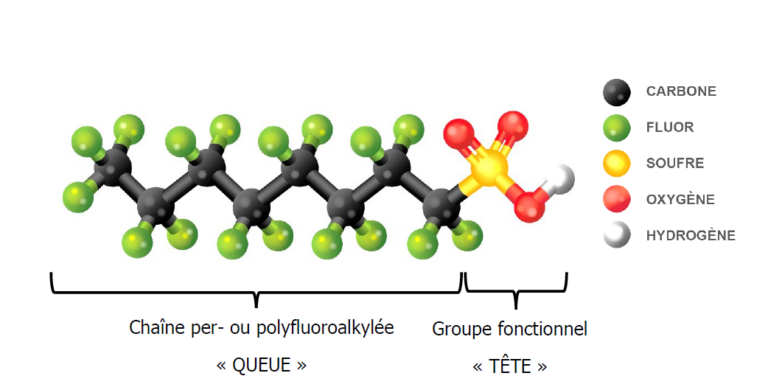
\includegraphics[width=0.82\linewidth]{Chap1/images/repre_pfas_polyflore.png}
    \caption{Repr\'esentation sch\'ematique du PFOS (acide perfluorooctanesulfonique, C$_8$F$_{17}$SO$_3$H ou C$_8$F$_{17}$SO$_3^-$). Source : adapt\'e de~\cite{vds2025pfas}.}
    \label{fig:pfos-structure}
\end{figure}
La structure illustr\'ee met en \'evidence la dualit\'e de la cha\^ine perfluor\'ee (queue) et du groupe sulfonate (t\^ete polaire), qui fonde \`a la fois la persistance et la tensioactivit\'e du compos\'e.

La \textbf{longueur de cha\^ine} modifie la solubilit\'e, la mobilit\'e et la bioaccumulation : les cha\^ines courtes se d\'eplacent plus facilement dans l'eau ; les cha\^ines longues sont davantage retenues par les mati\`eres organiques du sol et les prot\'eines.


\mySubSection{Usages, sources et devenir environnemental}{}
\label{sec:pfas-usages-sources}
\label{sec:pfas-usages}
\label{sec:pfas-transport}

La pr\'esence des PFAS dans l'environnement d\'ecoule d'une cha\^ine causale continue : des choix industriels engendrent des rejets, qui alimentent des sources de contamination, lesquelles propagent les compos\'es vers les milieux r\'ecepteurs selon des m\'ecanismes physiques bien document\'es.
Cette sous-section d\'etaille successivement les usages \`a l'origine des \'emissions, la nature des sources, les voies de dispersion, et le mod\`ele conceptuel source-voie-r\'ecepteur qui en synth\'etise la logique.


\mySubSubSection{Usages industriels}{}

Les PFAS ne sont pas des polluants accidentels ponctuels : ils r\'esultent de \textbf{choix industriels} r\'ep\'et\'es sur plus de soixante ans.
Leur combinaison de r\'epellence (eau, graisses), de stabilit\'e thermique et de faible friction a conduit \`a de nombreuses applications~\cite{gluge2020pfas} :
\begin{itemize}
    \item \textbf{Textiles et habillement} : imperm\'eabilit\'e, r\'esistance aux taches ;
    \item \textbf{Emballages alimentaires} et papier trait\'e : barri\`ere \`a l'huile et \`a l'eau ;
    \item \textbf{Mousses anti-incendie} pour feux d'hydrocarbures (films aqueux AFFF) ;
    \item \textbf{Industrie chimique et \'electronique} : fluides de proc\'ed\'e, lubrifiants, rev\^etements ;
    \item \textbf{Cosm\'etiques et produits d'entretien} : certains compos\'es sont aujourd'hui progressivement interdits ou restreints selon les juridictions.
\end{itemize}

\`A chaque \textbf{cycle de vie} (fabrication, utilisation, traitement des d\'echets), une fraction des PFAS peut \^etre rejet\'ee dans l'air, l'eau ou les sols.
Les proc\'ed\'es de traitement classiques des eaux us\'ees ou des lixiviats de d\'echarges ne sont g\'en\'eralement pas con\c{c}us pour \textbf{casser} la liaison C--F : une partie des compos\'es traverse les stations et retourne vers les milieux naturels~\cite{hu2016pfas,prevedouros2006pfas}.


\mySubSubSection{Typologie des sources de contamination}{}

On classe couramment les sources selon leur intensit\'e et leur localisation :
\begin{enumerate}
    \item \textbf{Sources ponctuelles industrielles} : usines de synth\`ese ou de transformation de produits fluor\'es, rejets historiques stock\'es dans les sols ;
    \item \textbf{Sites militaires et a\'eroportuaires} : entra\^inements au feu avec mousses AFFF, souvent identifi\'es comme \textbf{hotspots} de contamination des nappes ;
    \item \textbf{Sources diffuses} : stations d'\'epuration, sites d'enfouissement, ruissellement urbain transportant des r\'esidus de produits de consommation.
\end{enumerate}

Des \'etudes \`a l'\'echelle r\'egionale ont montr\'e une association statistique entre la pr\'esence de PFAS dans l'eau potable et la proximit\'e d'installations industrielles, de bases militaires ou de stations d'\'epuration~\cite{hu2016pfas}.
La mousse \textbf{AFFF} m\'erite une attention particuli\`ere : d\'evelopp\'ee pour \'eteindre les feux de carburant, elle a \'et\'e d\'eploy\'ee \`a grande \'echelle sur les a\'erodromes et casernes ; les m\'elanges infiltr\'es dans le sol peuvent alimenter des panaches souterrains durables.


\mySubSubSection{M\'ecanismes de transport dans l'air, le sol et l'eau}{}

Une fois rejet\'es, les PFAS suivent des trajectoires \textbf{coupl\'ees} :
\begin{itemize}
    \item \textbf{Eaux souterraines} : transport principalement \textbf{advectif} avec le flux de la nappe ; la vitesse d\'epend de la conductivit\'e hydraulique, de la porosit\'e, du gradient hydraulique et du degr\'e de r\'etention sur les sols (mati\`ere organique, min\'eraux)~\cite{brusseau2019pfas}.
    \item \textbf{Zone vadose} (non satur\'ee) : accumulation possible aux interfaces air--eau, formant un \textbf{r\'eservoir} lib\'er\'e progressivement lors des pluies ;
    \item \textbf{Atmosph\`ere} : certains pr\'ecurseurs volatils (fluorot\'elom\`eres) peuvent \^etre transport\'es sur de longues distances avant d\'ep\^ot sec ou humide, contribuant \`a une contamination \textbf{ubiquitaire} m\^eme loin des sites industriels~\cite{guelfo2021pfas}.
\end{itemize}

Sur des aquif\`eres perm\'eables \`a faible teneur en carbone, des panaches de plusieurs \textbf{kilom\`etres} ont \'et\'e d\'ecrits en aval de sources ponctuelles.
Le comportement ne se r\'eduit donc pas \`a une dilution imm\'ediate : la persistance et la mobilit\'e conjointes expliquent l'\'etendue spatiale des probl\`emes.


\mySubSubSection{Le sch\'ema source, voie et r\'ecepteur}{}
\label{sec:pfas-svr}

En \'evaluation des risques environnementaux, le devenir des PFAS est souvent repr\'esent\'e par le mod\`ele \textbf{source, voie et r\'ecepteur}~\cite{brusseau2019pfas,guelfo2021pfas} :
\begin{itemize}
    \item \textbf{Source} : activit\'e humaine qui \'emet les PFAS (usine, base militaire, rejet urbain) ;
    \item \textbf{Voie} : milieu qui transporte le polluant (sol, eau souterraine, eau de surface, air) ;
    \item \textbf{R\'ecepteur} : milieu ou organisme expos\'e (nappe exploit\'ee, puits, rivi\`ere, population).
\end{itemize}

Ce sch\'ema aide \`a structurer la pens\'ee, ind\'ependamment des outils math\'ematiques utilis\'es ensuite pour l'analyse des donn\'ees.
La figure~\ref{fig:voies-contamination-pfas} en illustre la d\'eclinaison concr\`ete pour les PFAS.

\begin{figure}[htbp]
    \centering
    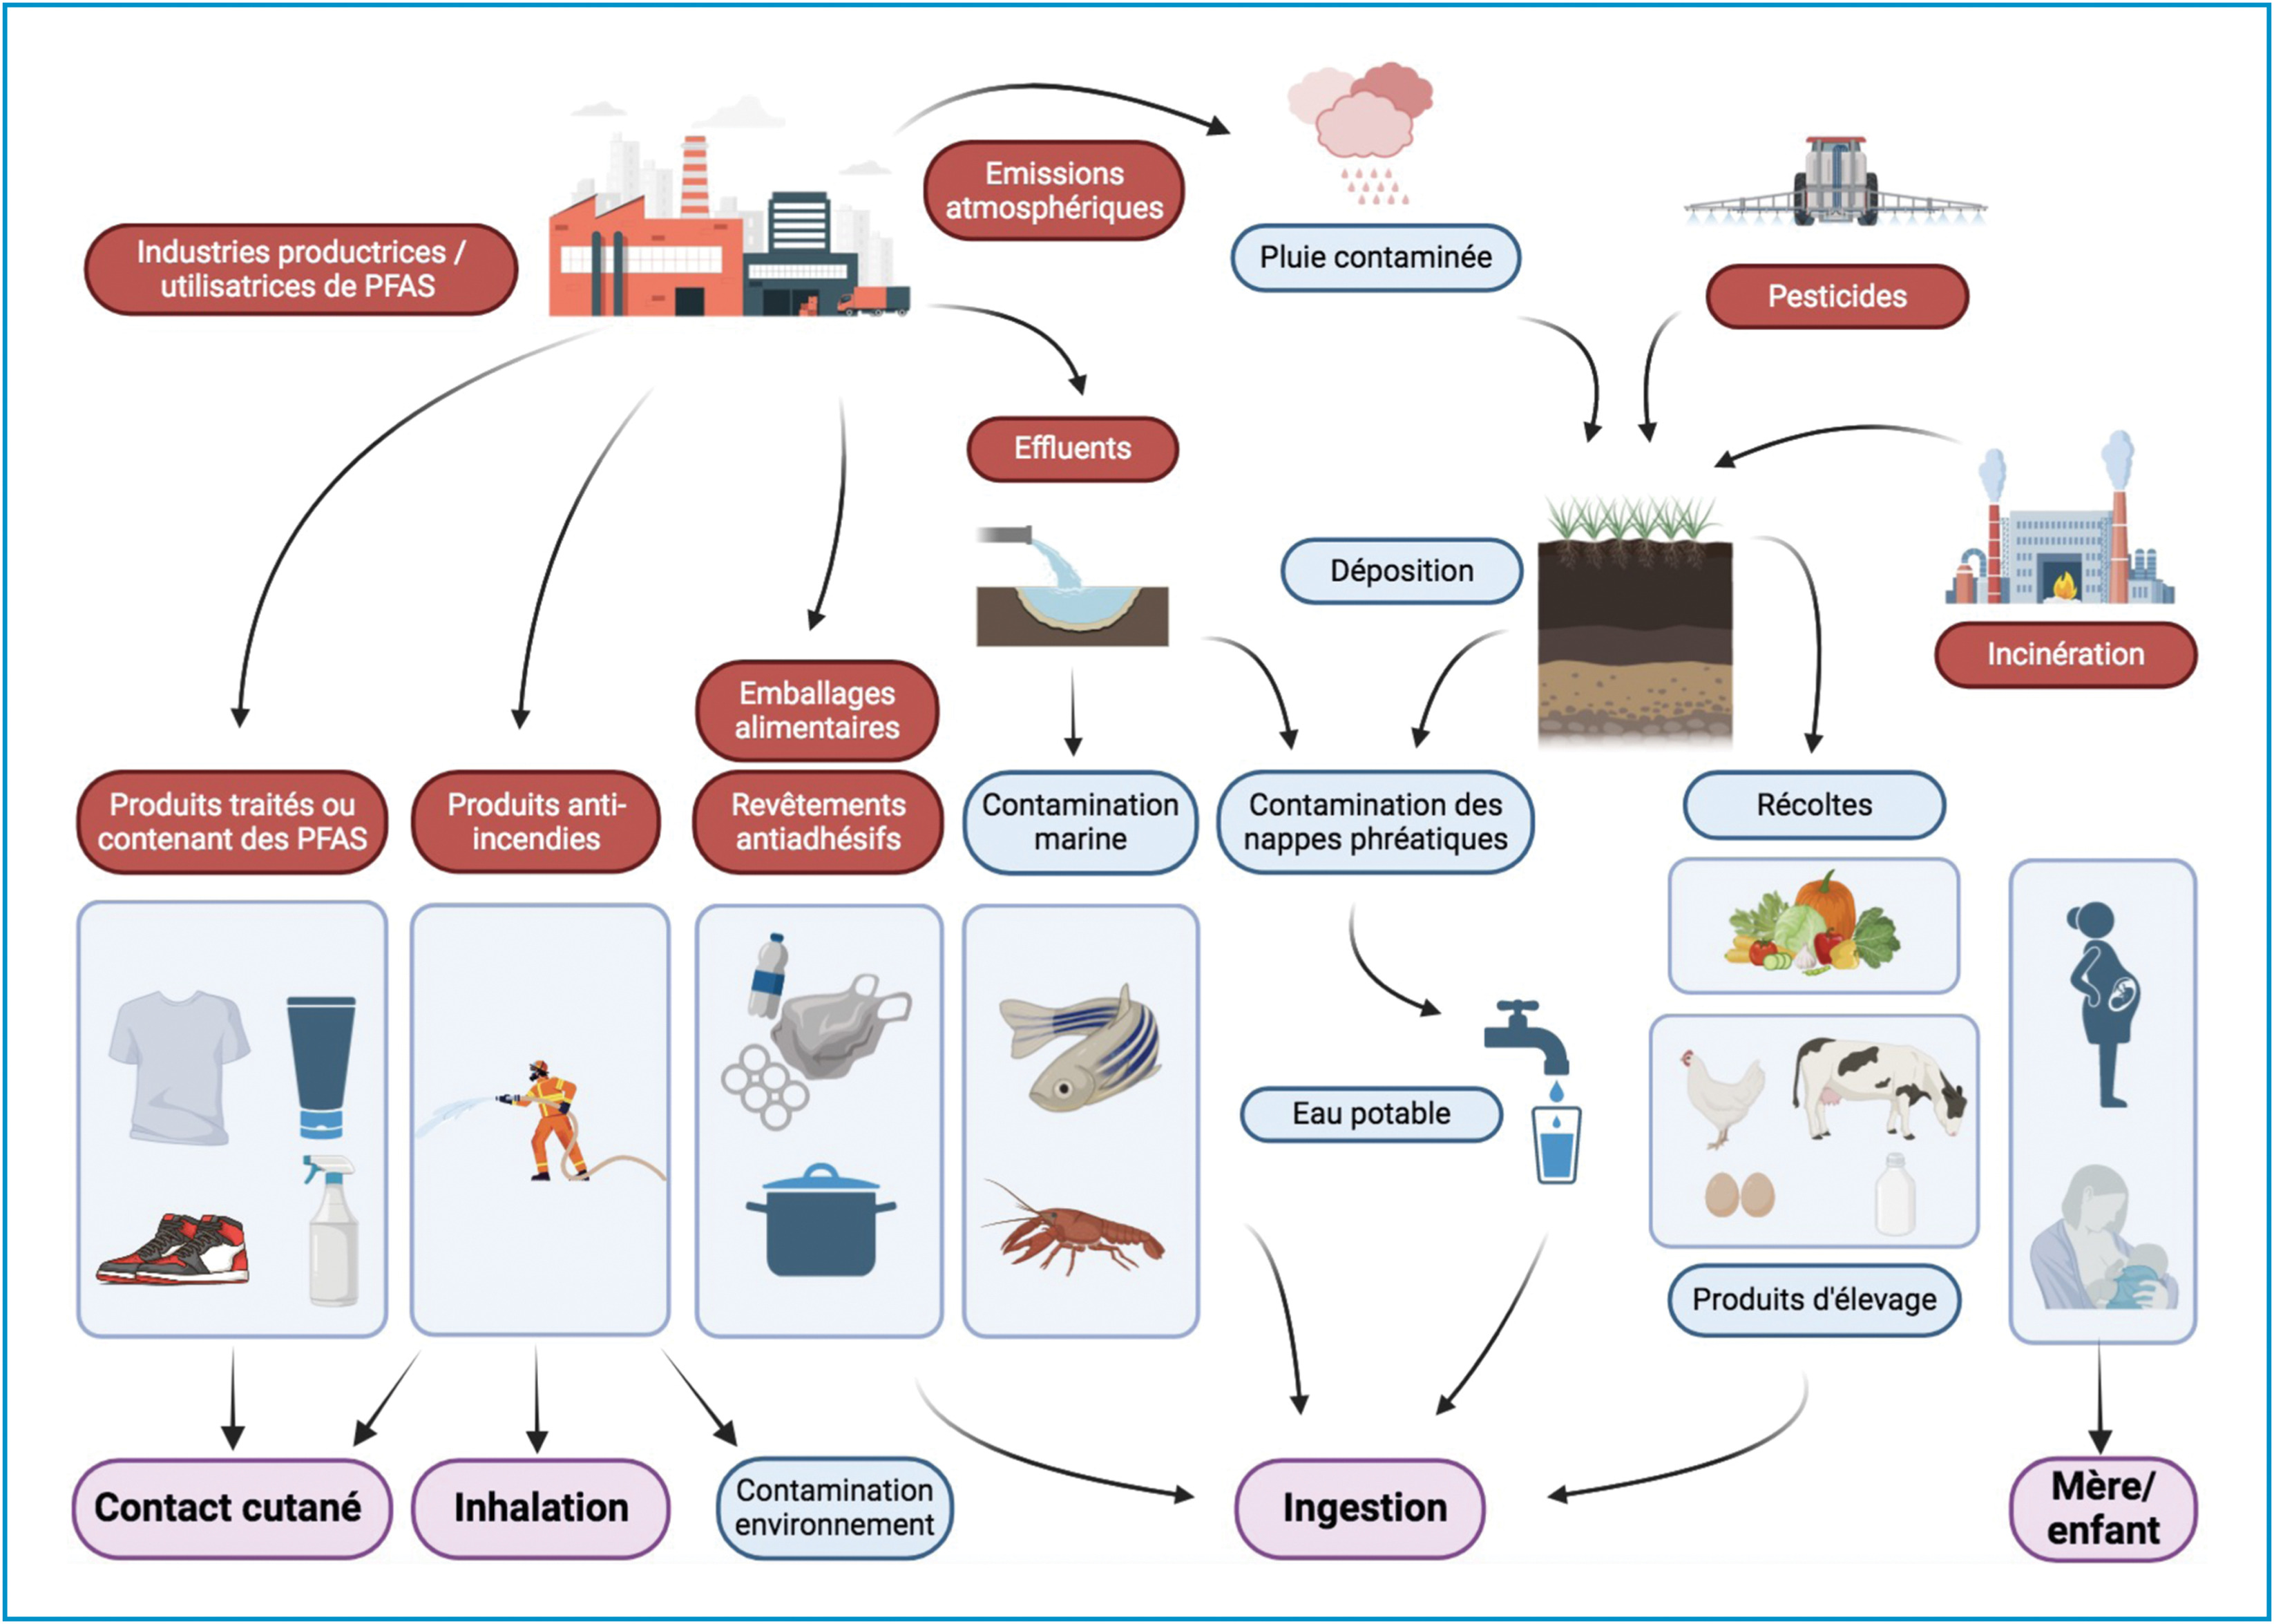
\includegraphics[width=0.92\linewidth]{Chap1/images/voie_contamination_pfas.jpg}
    \caption{Voies possibles de contamination humaine aux PFAS (sources directes en rouge, contamination indirecte via sol ou eau en bleu, voies d'exposition en violet). Source : adapt\'e de~\cite{fct2024pfasfigures}.}
    \label{fig:voies-contamination-pfas}
\end{figure}

La figure met en \'evidence que les rejets industriels ou l'usage de produits de consommation alimentent d'abord les milieux (sol, eau), avant d'atteindre l'homme par l'eau potable, l'alimentation ou d'autres voies d'exposition.
On observe par ailleurs une \textbf{co-occurrence} fr\'equente avec d'autres polluants organiques sur les m\^emes sites : solvants chlor\'es (TCE, PCE), hydrocarbures, additifs (MTBE).
Ces co-contaminants partagent souvent une histoire industrielle commune, m\^eme si leurs propri\'et\'es de transport diff\`erent.


\mySubSection{Surveillance des eaux souterraines et limites de la mesure}{}
\label{sec:pfas-surveillance}

Les \textbf{eaux souterraines} constituent un enjeu majeur car elles alimentent une part importante de l'eau potable et de l'irrigation.
Les PFAS y sont d'autant plus pr\'eoccupants qu'ils peuvent migrer \textbf{loin} de la source visible et demeurer longtemps \`a des concentrations tr\`es faibles mais significatives sur le plan sanitaire~\cite{hu2016pfas}.

La \textbf{surveillance} repose classiquement sur :
\begin{itemize}
    \item le pr\'el\`evement sur des \textbf{puits} ou points de contr\^ole ;
    \item l'analyse en laboratoire par chromatographie de type LC-MS/MS, ciblant un \textbf{panier} de compos\'es (souvent quelques dizaines de mol\'ecules parmi des milliers possibles) ;
    \item la comparaison aux \textbf{seuils r\'eglementaires} ou aux valeurs guides sanitaires.
\end{itemize}

Plusieurs limites structurelles expliquent la difficult\'e d'un suivi exhaustif :
\begin{itemize}
    \item \textbf{Co\^ut} \'elev\'e d'une analyse multi-compos\'es ;
    \item \textbf{Couverture spatiale} incompl\`ete (impossible de mesurer tous les puits d'une r\'egion) ;
    \item \textbf{Non-d\'etection} fr\'equente : une valeur nulle ne signifie pas toujours l'absence de PFAS, mais parfois une concentration sous le seuil de d\'etection de la m\'ethode~\cite{guelfo2021pfas} ;
    \item \textbf{H\'et\'erog\'en\'eit\'e} des protocoles entre r\'egions et campagnes.
\end{itemize}

Ces contraintes expliquent l'int\'er\^et, dans la litt\'erature r\'ecente, pour des approches de \textbf{priorisation} fond\'ees sur des donn\'ees d\'ej\`a disponibles (contexte g\'eologique, proximit\'e d'activit\'es, qualit\'e de l'eau)~\cite{dong2024pfas}.


\mySubSection{Impacts sanitaires et cadre r\'eglementaire}{}
\label{sec:pfas-reglementation}

\mySubSubSection{Voies d'exposition et effets document\'es}{}

L'exposition humaine aux PFAS peut intervenir par plusieurs \textbf{voies}~\cite{sunderland2019pfas} :
\begin{itemize}
    \item \textbf{Eau potable} contamin\'ee (voie souvent dominante pr\`es des sites pollu\'es) ;
    \item \textbf{Alimentation} (poissons d'eau douce, produits d'origine animale bioaccumulants) ;
    \item \textbf{Poussi\`eres int\'erieures} et produits de consommation trait\'es ;
    \item \textbf{Contact professionnel} sur les sites de production ou d'usage intensif.
\end{itemize}

Les effets sanitaires \'etudi\'es \`a des doses environnementales tr\`es basses (ng/L dans l'eau) incluent notamment :
\begin{itemize}
    \item des effets sur le \textbf{syst\`eme immunitaire} (r\'eponse vaccinale);
    \item des perturbations \textbf{thyro\"idiennes} et m\'etaboliques (lipides);
    \item des impacts sur le \textbf{d\'eveloppement f\oe tal} (poids \`a la naissance, pr\'e\'eclampsie);
    \item pour certains compos\'es, des associations avec des \textbf{cancers} (rein, testicules) dans les cohortes les plus expos\'ees.
\end{itemize}

La figure~\ref{fig:pfas-pathologies} synth\'etise les pathologies suspect\'ees d'\^etre li\'ees \`a la toxicit\'e des PFAS chez l'humain.

\begin{figure}[H]
    \centering
    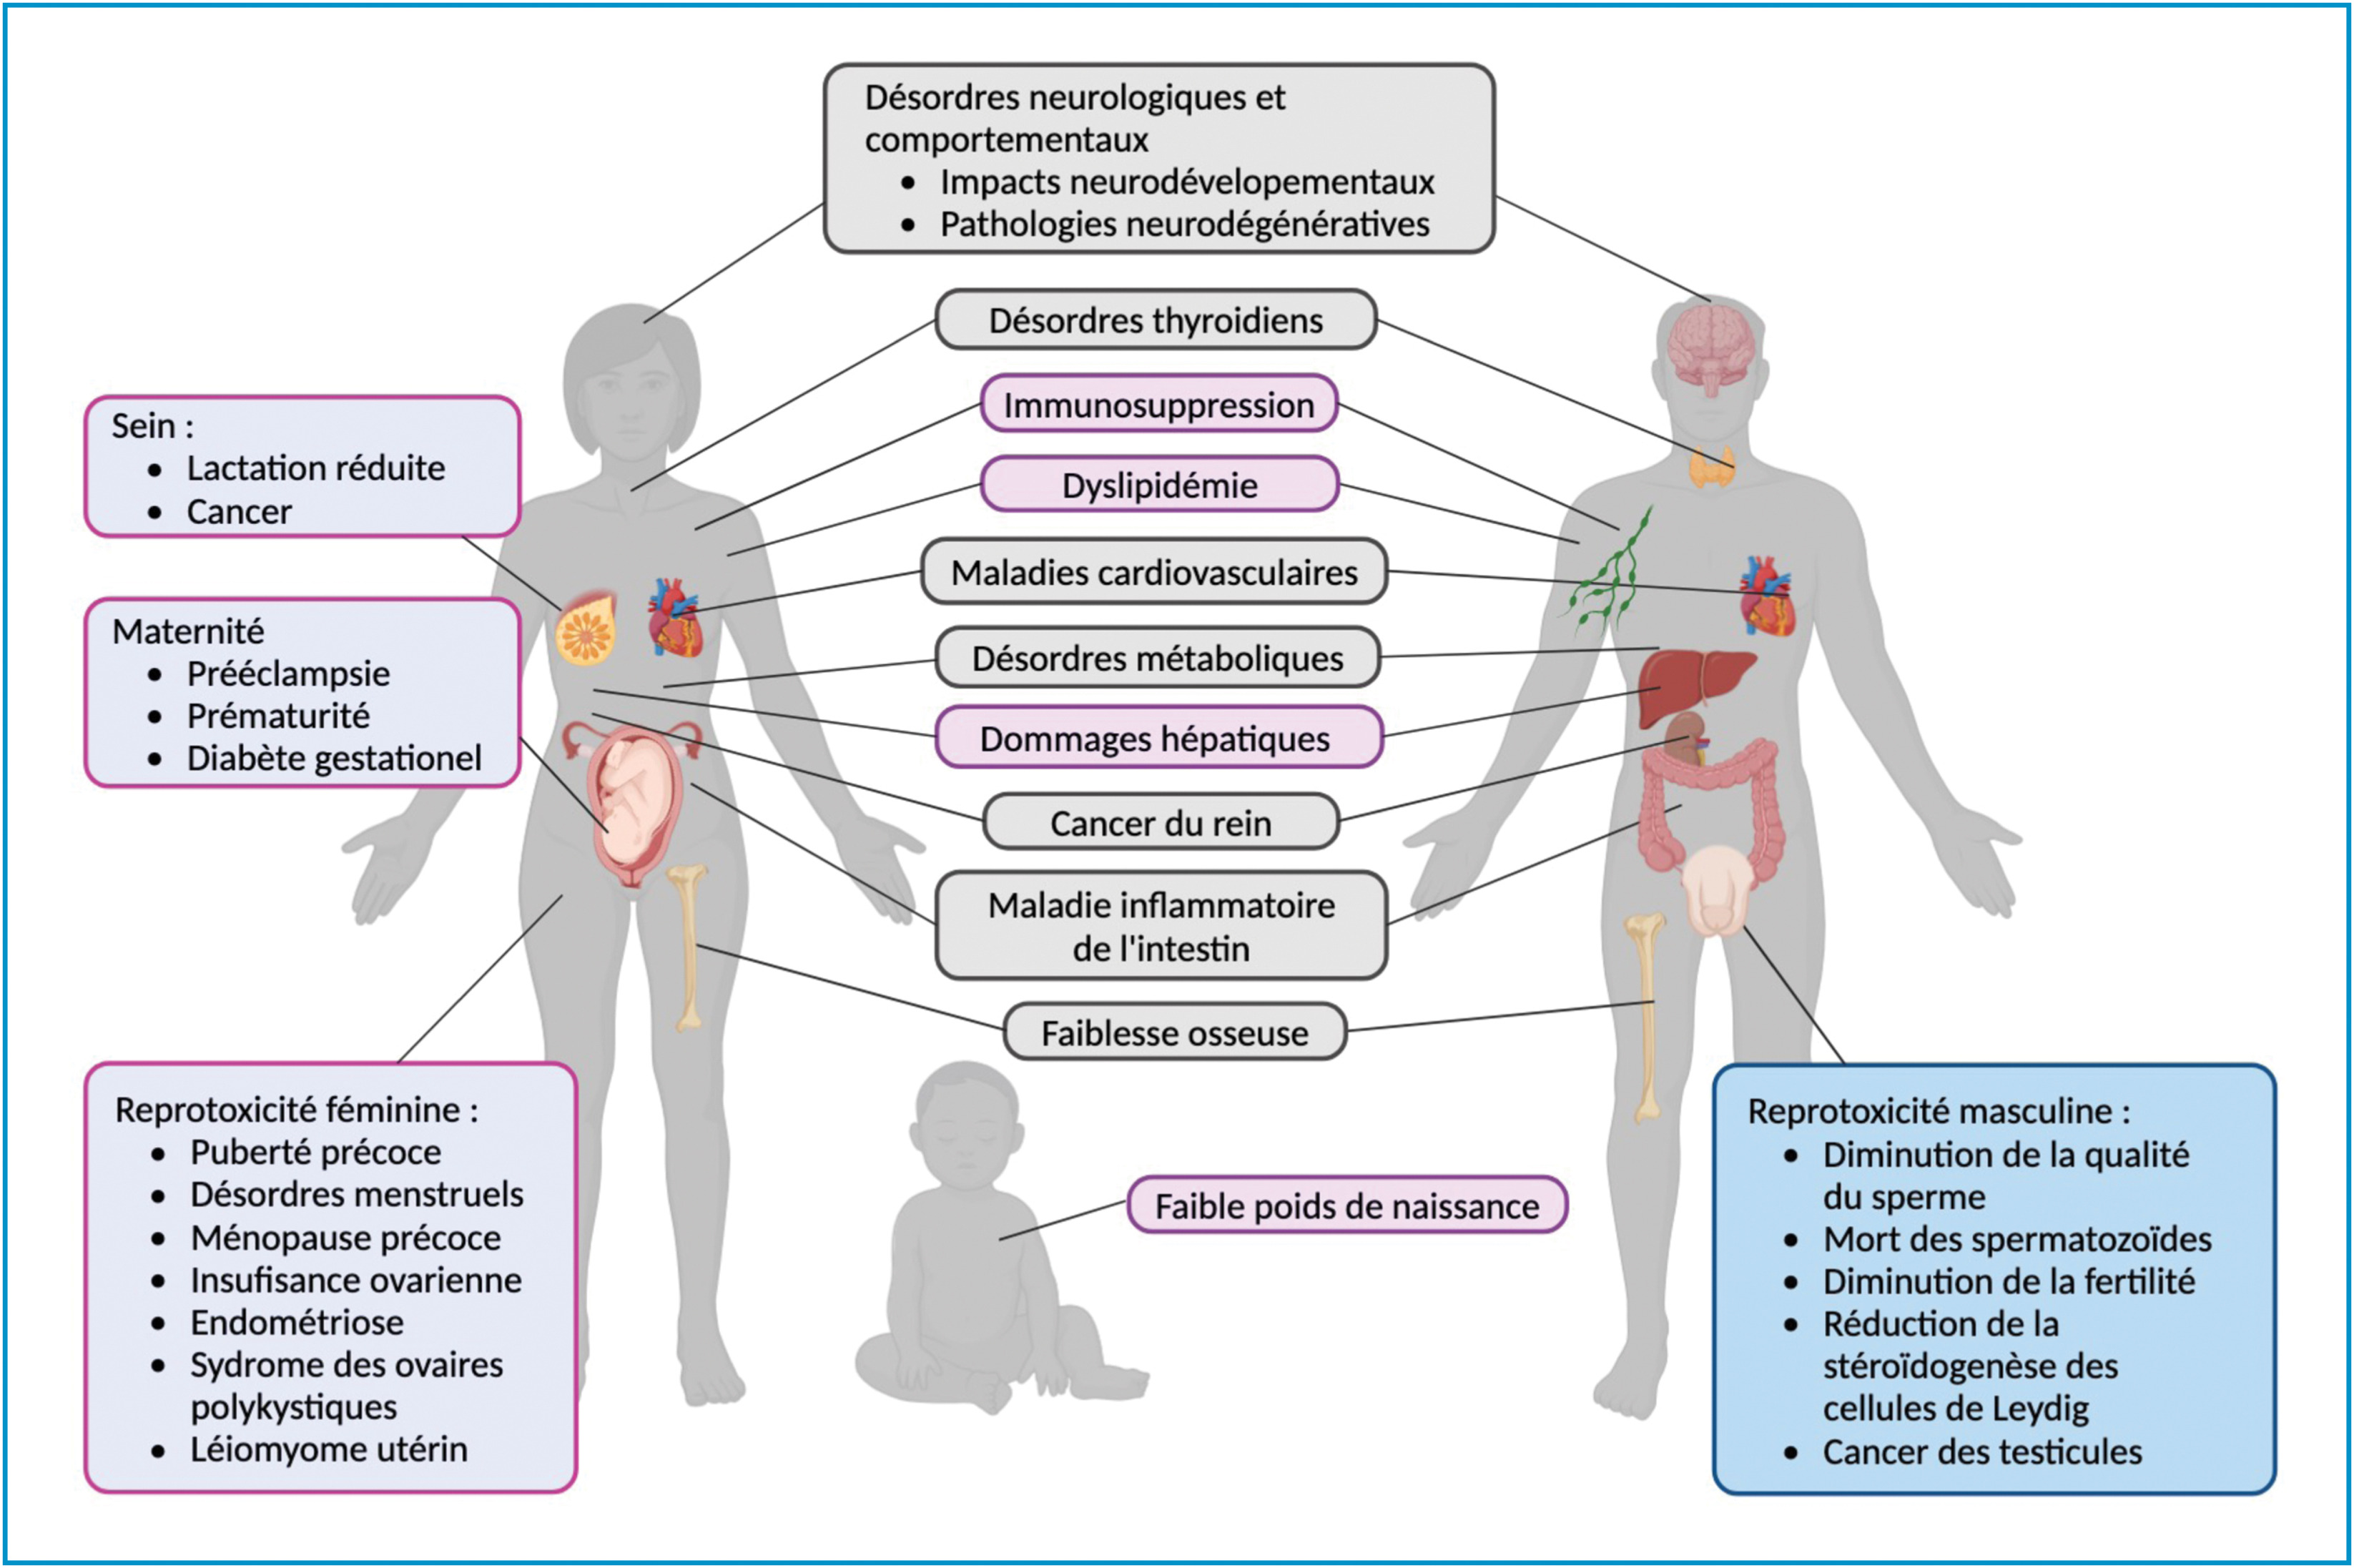
\includegraphics[width=0.88\linewidth]{Chap1/images/human_pfas_pathologies.jpg}
    \caption{Pathologies suspect\'ees d'\^etre induites par la toxicit\'e des PFAS (effets \'epid\'emiologiques corrobor\'es au centre ; autres effets document\'es en gris ; effets reprotoxiques sur les c\^ot\'es). Source : adapt\'e de~\cite{fct2024pfasfigures}.}
    \label{fig:pfas-pathologies}
\end{figure}
Cette synth\`ese illustre que plusieurs organes et fonctions (immunit\'e, thyro\"ide, d\'eveloppement f\oe tal, reproduction) figurent parmi les effets les plus document\'es, justifiant le renforcement des seuils r\'eglementaires et des programmes de surveillance.

Le tableau~\ref{tab:pfas-sante} en donne une vue synth\'etique tabulaire ; il ne remplace pas une analyse toxicologique d\'etaill\'ee.

\begin{table}[h!]
    \centering
    \caption{Exemples d'effets sanitaires associ\'es \`a l'exposition aux PFAS (synth\`ese).}
    \label{tab:pfas-sante}
    \begin{tabular}{lp{5.5cm}p{4cm}}
        \hline
        Syst\`eme & Effets document\'es & Populations sensibles \\
        \hline
        Immunitaire & Diminution de la r\'eponse vaccinale & Enfants \\
        Endocrinien & Perturbation thyro\"idienne, lipides & Adultes \\
        D\'eveloppement & Faible poids \`a la naissance & Femmes enceintes \\
        Reproduction & Fertilit\'e, complications gestationnelles & Adultes \\
        Canc\'er (certains compos\'es) & Rein, testicules (associations) & Expos\'es professionnels \\
        \hline
    \end{tabular}
\end{table}


\mySubSubSection{\'Evolution du cadre r\'eglementaire}{}

Face \`a ces risques, les seuils admissibles ont fortement baiss\'e au cours des derni\`eres ann\'ees.
Aux \'Etats-Unis, l'EPA a publi\'e en 2016 un \textbf{avis sanitaire} (\emph{health advisory}) \`a \textbf{70~ng/L} pour la somme PFOA+PFOS~\cite{epa2016pfas}, puis en 2024 un \textbf{r\`eglement national} sur l'eau potable fixant des limites maximales de contaminants (MCL) \`a \textbf{4~ng/L} pour le PFOA et le PFOS \textbf{s\'epar\'ement}~\cite{epa2023npdwr}.
Cette dualit\'e (avis historique vs limites r\'ecentes plus strictes) illustre la \textbf{rapidit\'e} de l'\'evolution normative.

En Europe, la directive sur l'eau potable (2020/2184/UE) encadre un sous-ensemble de PFAS :
\begin{itemize}
    \item une limite sur la \textbf{somme de 20 PFAS} prioritaires (indicateur \texttt{PFAS Total}, valeur param\'etrique de l'ordre de 0,1~$\mu$g/L) ;
    \item une limite sur le \textbf{total des PFAS} mesur\'es au-del\`a d'un seuil de quantification (indicateur \texttt{PFAS TQS}, de l'ordre de 0,5~$\mu$g/L).
\end{itemize}

Des initiatives nationales compl\`etent ce cadre (programmes de surveillance en Allemagne, Pays-Bas, Danemark, etc.).
En France, des textes r\'ecents visent \`a restreindre certains usages non essentiels (cosm\'etiques, textiles, produits de loisirs) et \`a renforcer la fiscalit\'e ou la redevance sur les rejets industriels, dans une logique de \textbf{pr\'evention} \`a la source.

Quelle que soit la juridiction, le message commun est le suivant : les concentrations d'int\'er\^et sont \textbf{tr\`es faibles}, la liste des compos\'es \`a suivre \textbf{change}, et la surveillance doit \^etre \textbf{\'etendue} dans le temps et dans l'espace, ce qui pose un d\'efi logistique consid\'erable pour les gestionnaires de l'eau.

Sur le continent africain, les r\'eglementations nationales sp\'ecifiques aux PFAS font encore largement d\'efaut.
Les lignes directrices de l'Organisation mondiale de la sant\'e pour la qualit\'e de l'eau potable~\cite{who2022drinking} constituent, dans ce contexte, la r\'ef\'erence disponible pour les pays d'Afrique subsaharienne.
Au Cameroun en particulier, aucune norme nationale d\'edi\'ee aux PFAS n'est actuellement en vigueur ; la surveillance s'appuie sur des valeurs guides internationales, rendant d'autant plus pertinentes les approches fond\'ees sur des donn\'ees contextuelles disponibles pour estimer le risque sans analyse cibl\'ee syst\'ematique.

L'ensemble de ces contraintes (analytiques, logistiques et r\'eglementaires) motive le recours \`a des outils d'apprentissage automatique capables d'extraire un signal utile \`a partir des donn\'ees existantes.
La section suivante introduit les m\'ethodes et paradigmes de l'apprentissage automatique qui seront mobilis\'es dans cette \'etude.

\mySection{Apprentissage automatique et m\'ethodes d'ensemble}{}
\label{sec:ml-ensemble}

L'\textbf{apprentissage automatique} (\emph{machine learning}, ML) regroupe les m\'ethodes qui permettent \`a un syst\`eme informatique d'am\'eliorer une t\^ache \`a partir de donn\'ees, sans que chaque r\`egle de d\'ecision soit cod\'ee explicitement.
En sciences de l'environnement, ces approches servent notamment \`a exploiter des tableaux de mesures et de variables contextuelles (g\'eologie, hydrologie, proximit\'e d'activit\'es) pour estimer un risque ou prioriser des sites \`a contr\^oler.
Cette section pr\'esente d'abord les principaux \textbf{paradigmes} d'apprentissage, puis les \textbf{principes des m\'ethodes d'ensemble} illustr\'es par des exemples courants.


\mySubSection{Paradigmes de l'apprentissage automatique}{}
\label{sec:ml-definition}

L'apprentissage automatique peut se d\'efinir, suivant Mitchell~\cite{mitchell1997ml}, comme suit : un programme \textbf{apprend} \`a partir de l'exp\'erience $E$ par rapport \`a une classe de t\^aches $T$ et une mesure de performance $P$ si sa performance sur $T$, mesur\'ee par $P$, s'am\'eliore avec l'accumulation de l'exp\'erience $E$.
En pratique, un \textbf{algorithme} ajuste des param\`etres \`a partir d'exemples pour produire des pr\'edictions ou des d\'ecisions.
On distingue ensuite plusieurs paradigmes selon la nature des donn\'ees disponibles et l'objectif vis\'e.


\mySubSubSection{Apprentissage supervis\'e}{}
\label{sec:ml-supervise}

En \textbf{apprentissage supervis\'e}, chaque exemple d'entr\'ee $\mathbf{x}$ est associ\'e \`a une \textbf{\'etiquette} $y$ connue.
L'objectif est d'apprendre une fonction $f(\mathbf{x}) \approx y$ qui \textbf{g\'en\'eralise} \`a de nouvelles observations non vues \`a l'entra\^inement.

Deux t\^aches principales en d\'ecoulent :
\begin{itemize}
    \item la \textbf{classification}, lorsque $y$ est discr\`ete (par exemple \emph{contamin\'e} / \emph{non contamin\'e}) ;
    \item la \textbf{r\'egression}, lorsque $y$ est continue (par exemple une concentration mesur\'ee).
\end{itemize}

Le protocole habituel consiste \`a s\'eparer les donn\'ees en un jeu d'\textbf{entra\^inement} (pour ajuster $f$), un jeu de \textbf{validation} (pour choisir les hyperparam\`etres) et un jeu de \textbf{test} (pour estimer la performance en conditions ind\'ependantes).
En surveillance environnementale, la classification binaire (d\'epassement ou non d'un seuil, pr\'esence ou absence d'un signal) est fr\'equente lorsque l'on cherche \`a orienter des campagnes de mesure~\cite{hastie2009elements}.


\mySubSubSection{Apprentissage non supervis\'e}{}
\label{sec:ml-non-supervise}

En \textbf{apprentissage non supervis\'e}, les donn\'ees ne sont pas \'etiquet\'ees : l'algorithme cherche \`a mettre en \'evidence des \textbf{structures} sans cible explicite~\cite{hastie2009elements}.
Les objectifs typiques sont :
\begin{itemize}
    \item le \textbf{regroupement} (\emph{clustering}), par exemple regrouper des sites aux profils hydrog\'eologiques voisins ;
    \item la \textbf{r\'eduction de dimension}, pour visualiser ou compresser un grand nombre de variables corr\'el\'ees ;
    \item la d\'etection d'\textbf{anomalies}, pour rep\'erer des observations atypiques.
\end{itemize}

Ces m\'ethodes ne produisent pas directement une pr\'ediction de contamination, mais elles peuvent pr\'ec\'eder une \'etape supervis\'ee en r\'ev\'elant des homog\'en\'eit\'es spatiales ou des corr\'elations entre variables.


\mySubSubSection{Apprentissage semi-supervis\'e}{}
\label{sec:ml-semi-supervise}

L'\textbf{apprentissage semi-supervis\'e} combine un nombre limit\'e d'exemples \textbf{\'etiquet\'es} et un volume plus important de donn\'ees \textbf{non \'etiquet\'ees}.
Il est particuli\`erement utile lorsque l'\'etiquetage est \textbf{co\^uteux} ou \textbf{lent}, ce qui est souvent le cas en environnement lorsque chaque \'etiquette correspond \`a une analyse de laboratoire.

L'id\'ee g\'en\'erale est d'exploiter la structure des donn\'ees non \'etiquet\'ees (similarit\'e entre sites, continuit\'e spatiale) pour renforcer un mod\`ele entra\^in\'e sur le sous-ensemble \'etiquet\'e.
Des travaux r\'ecents sur les PFAS en eaux souterraines ont mobilis\'e cette logique lorsque les mesures cibl\'ees restent rares par rapport au nombre de points \`a \'evaluer~\cite{dong2024pfas}.


\mySubSubSection{Apprentissage par renforcement}{}
\label{sec:ml-rl}

En \textbf{apprentissage par renforcement}, un \textbf{agent} interagit avec un \textbf{environnement} et apprend une politique de d\'ecision \`a partir de \textbf{r\'ecompenses} ou de \textbf{p\'enalit\'es} re\c{c}ues au fil du temps.
Contrairement au cadre supervis\'e, il n'existe pas d'\'etiquette correcte pour chaque action : l'agent doit \textbf{explorer} et \textbf{exploiter} ses choix pour maximiser un gain cumul\'e.

Ce paradigme trouve ses principales applications en robotique, dans les jeux \`a information incompl\`ete et dans les syst\`emes de recommandation dynamique~\cite{sutton2018rl}.


\mySubSection{M\'ethodes d'ensemble}{}
\label{sec:ensemble}

Une \textbf{m\'ethode d'ensemble} combine plusieurs \textbf{apprenants} pour former un pr\'edicteur plus stable ou plus pr\'ecis qu'un mod\`ele isol\'e.
Le principe est le suivant : si les apprenants ne se trompent pas toujours aux m\^emes endroits, les combiner peut compenser leurs faiblesses respectives.
Le \textbf{bagging} att\'enue surtout la \textbf{variance} (pr\'edictions instables d'un mod\`ele tr\`es flexible), tandis que le \textbf{boosting} r\'eduit plut\^ot le \textbf{biais} (erreurs syst\'ematiques d'un mod\`ele trop simple). Quant au \textbf{stacking}, il combine des mod\`eles de natures \'eventuellement diff\'erentes pour optimiser la combinaison des sorties.


\mySubSubSection{Bagging}{}
\label{sec:bagging}

Le \textbf{bagging} (\emph{bootstrap aggregating}) entra\^ine plusieurs mod\`eles en \textbf{parall\`ele} sur des tirages \textbf{bootstrap} des observations (\'echantillonnage avec remise), puis \textbf{agr\`ege} leurs pr\'edictions.
En classification, la d\'ecision finale est un \textbf{vote majoritaire} ; en r\'egression, une moyenne des pr\'edictions.
Le bagging vise surtout \`a stabiliser un apprenant \`a forte variance (comme un arbre de d\'ecision profond) en moyennant des versions entra\^in\'ees sur des sous-jeux l\'eg\`erement diff\'erents.
On peut formaliser l'agr\'egation en classification par
\[
\hat{y}(\mathbf{x}) = \operatorname*{arg\,max}_{c \in \mathcal{C}} \sum_{b=1}^{B} \mathbb{1}\!\left(h_b(\mathbf{x}) = c\right),
\]
o\`u $h_b$ d\'esigne le $b$-i\`eme mod\`ele entra\^in\'e sur un bootstrap, et $B$ le nombre total de mod\`eles.
Plus $B$ augmente, plus la pr\'ediction devient stable, jusqu'\`a un plateau de performance.


\textbf{Exemple (for\^et al\'eatoire).}
La \textbf{for\^et al\'eatoire} (\emph{Random Forest})~\cite{breiman2001rf} est l'illustration standard du bagging appliqu\'e aux arbres de d\'ecision.
Chaque arbre est entra\^in\'e sur un sous-\'echantillon bootstrap ; \`a chaque n\oe ud, seul un sous-ensemble al\'eatoire de variables est candidat au meilleur partage.
Cette double al\'ea (donn\'ees et variables) \textbf{d\'ecorr\`ele} les arbres et limite le surapprentissage.
Dans la pratique, les hyperparam\`etres les plus structurants sont :
\begin{itemize}
    \item le nombre d'arbres $B$ (\texttt{n\_estimators}) ;
    \item la profondeur maximale de chaque arbre (\texttt{max\_depth}) ;
    \item le nombre minimal d'observations pour scinder un n\oe ud ou cr\'eer une feuille (\texttt{min\_samples\_split}, \texttt{min\_samples\_leaf}) ;
    \item le nombre de variables test\'ees \`a chaque n\oe ud (\texttt{max\_features}).
\end{itemize}
Un r\'eglage prudent de ces param\`etres contr\^ole le compromis biais-variance et \'evite des arbres trop sp\'ecialis\'es.

Un atout important de Random Forest est l'estimation dite \textbf{out-of-bag} (OOB) : pour chaque observation, on peut \'evaluer la pr\'ediction en utilisant uniquement les arbres qui n'ont pas vu cette observation \`a l'entra\^inement.
Ce score OOB donne une estimation rapide de la g\'en\'eralisation sans validation crois\'ee exhaustive.

Pour l'interpr\'etation, la for\^et fournit des \textbf{importances de variables} (par impurit\'e ou par permutation), utiles pour identifier les descripteurs dominants.
En revanche, ces importances doivent \^etre analys\'ees avec prudence en pr\'esence de variables corr\'el\'ees.
Les for\^ets al\'eatoires restent ainsi une base solide en donn\'ees tabulaires, \`a la fois robuste, explicable \`a un niveau global, et souvent performante comme mod\`ele de r\'ef\'erence ou composant d'un ensemble plus complexe.

La figure~\ref{fig:random-forest-schema} illustre le principe d'une for\^et al\'eatoire : plusieurs arbres entra\^in\'es en parall\`ele sur des sous-\'echantillons, puis agr\'eg\'es par vote.

\begin{figure}[H]
    \centering
    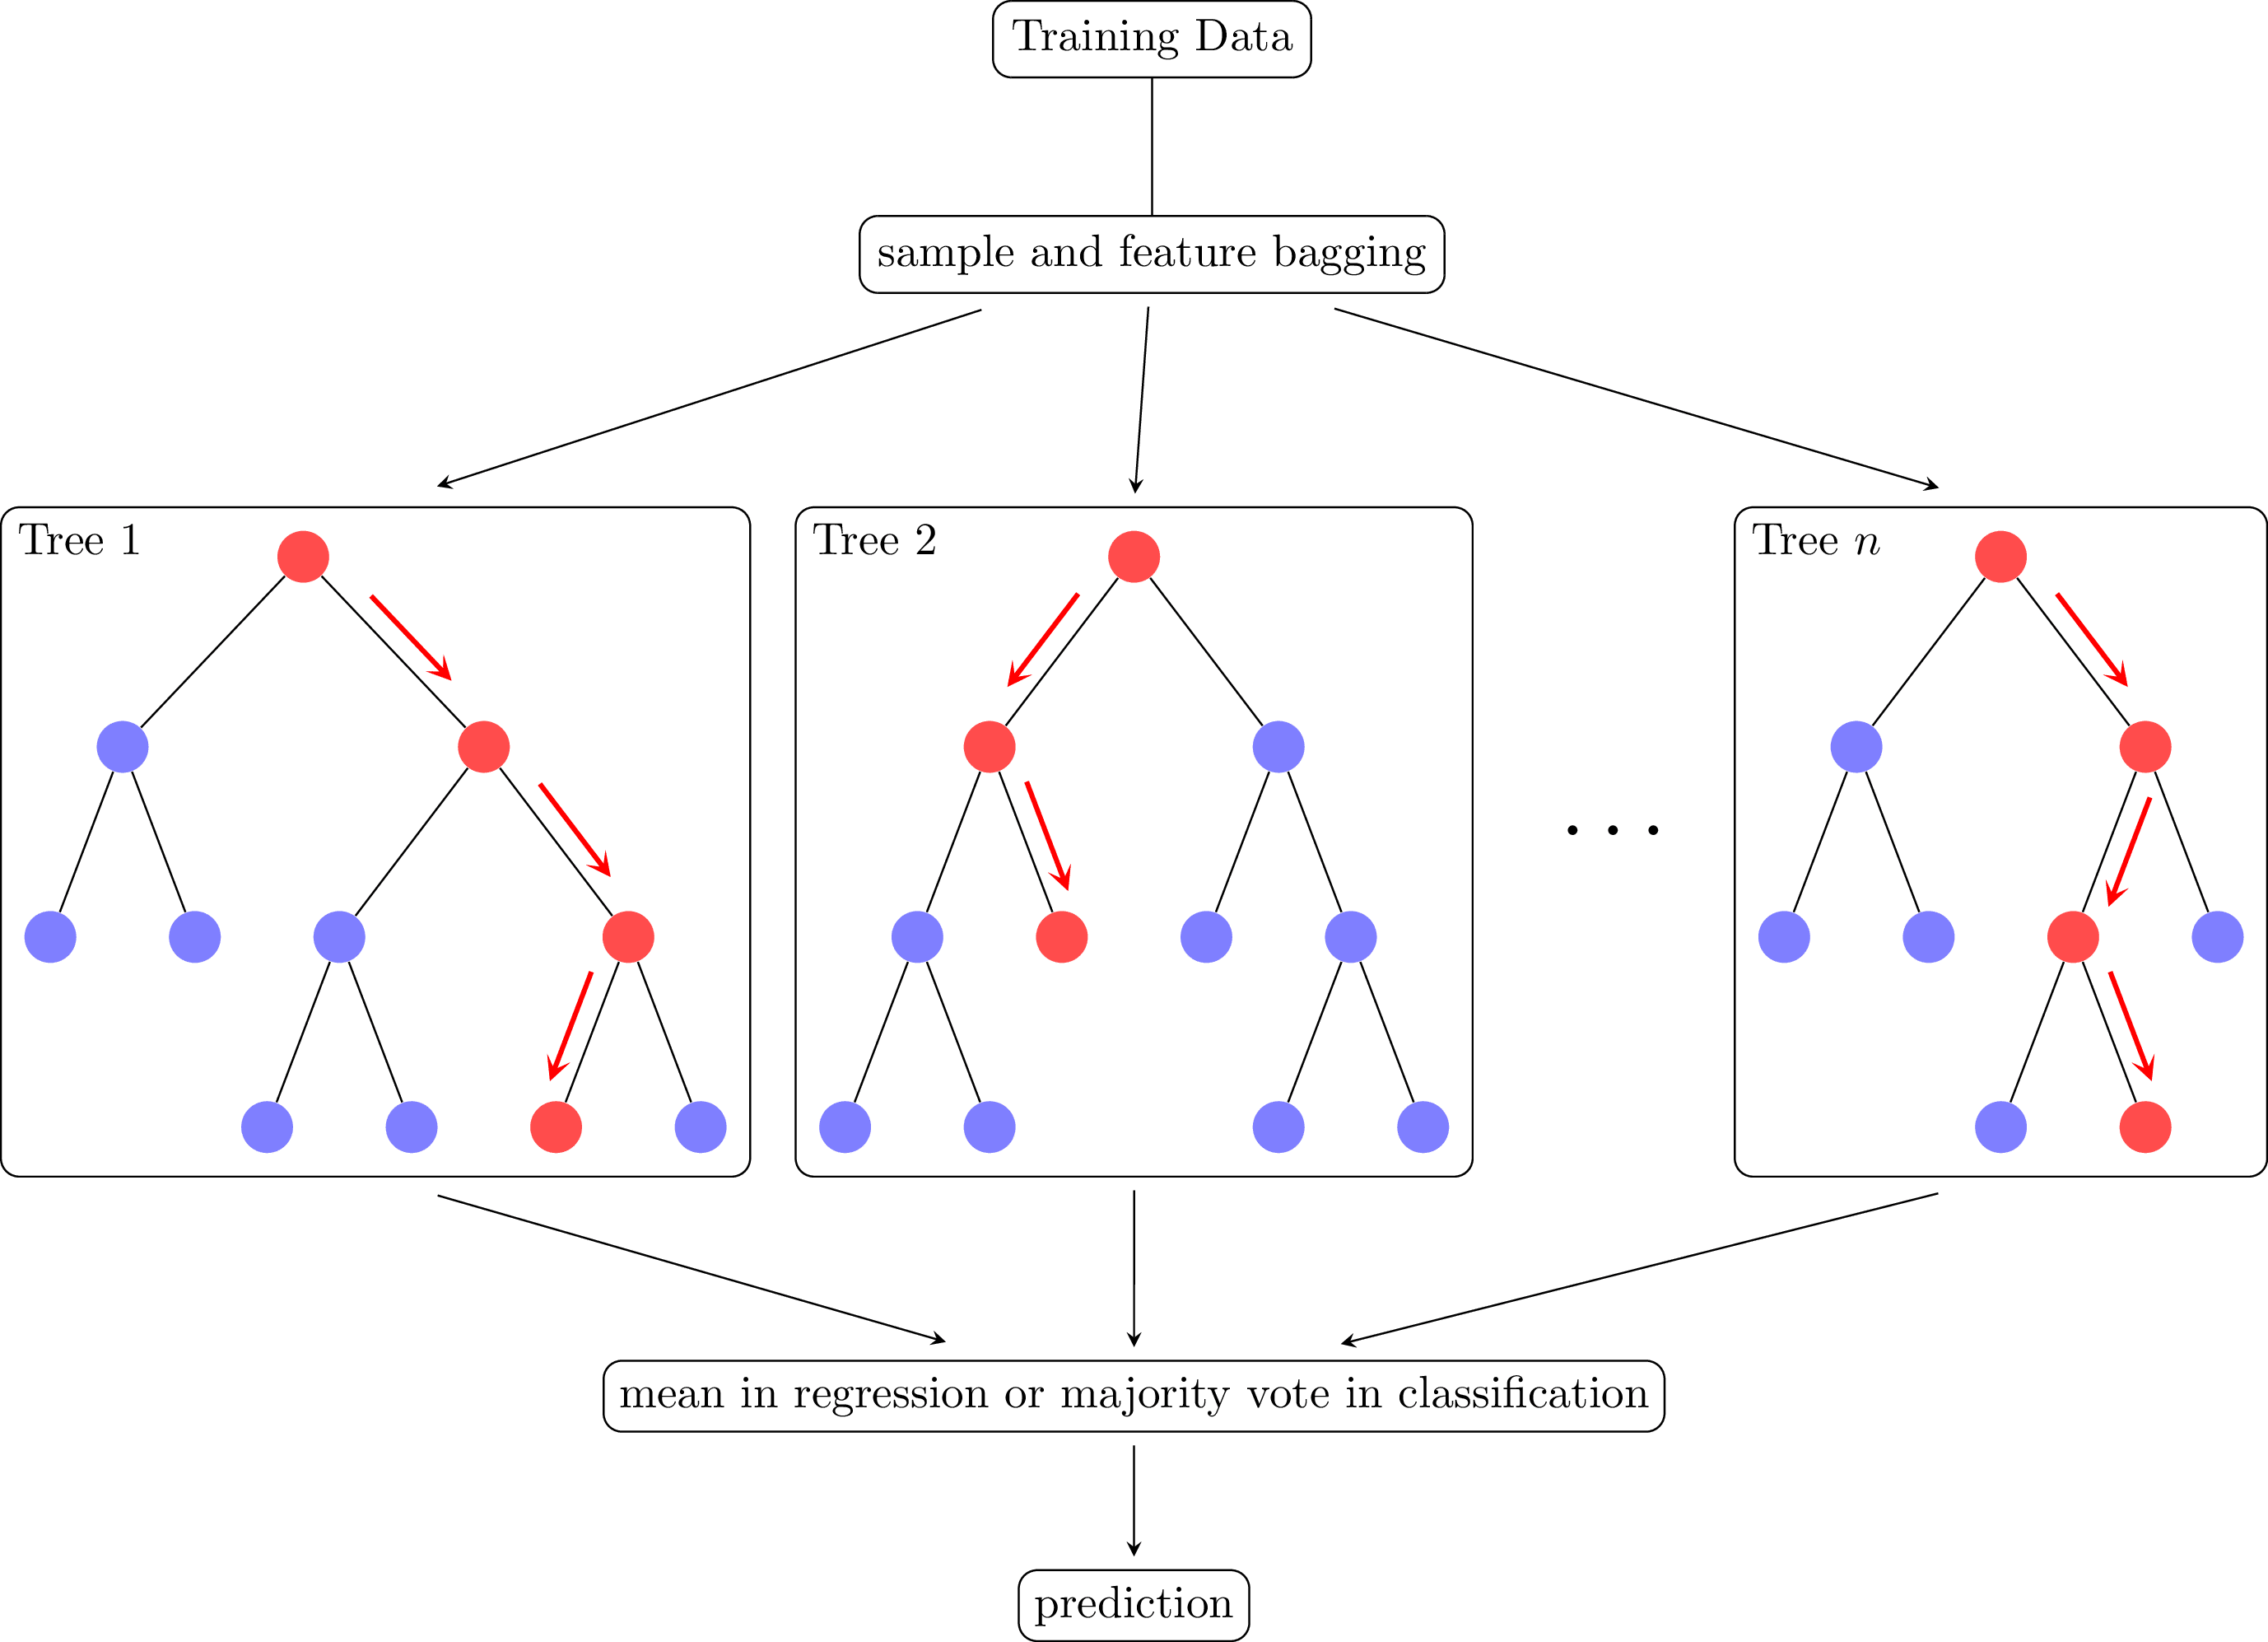
\includegraphics[width=0.88\linewidth]{Chap1/images/random-forest.png}
    \caption{Sch\'ema d'une for\^et al\'eatoire (bagging d'arbres de d\'ecision avec sous-\'echantillonnage des observations et des variables). Source : adapt\'e de~\cite{janosh2024randomforest}.}
    \label{fig:random-forest-schema}
\end{figure}
Chaque arbre voit un sous-jeu de donn\'ees diff\'erent et ne retient qu'une fraction des variables \`a chaque scission, ce qui diversifie les pr\'edictions avant leur agr\'egation finale.

\mySubSubSection{Boosting}{}
\label{sec:boosting}

Le \textbf{boosting} construit le mod\`ele de fa\c{c}on \textbf{s\'equentielle} : chaque nouvel apprenant cible les erreurs laiss\'ees par l'ensemble des apprenants pr\'ec\'edents, au lieu d'entra\^iner des mod\`eles ind\'ependants comme en bagging.
La figure~\ref{fig:boosting-schema} r\'esume cette logique additive : le mod\`ele courant est enrichi \`a chaque it\'eration par un arbre entra\^in\'e sur les r\'esidus.

\begin{figure}[H]
    \centering
    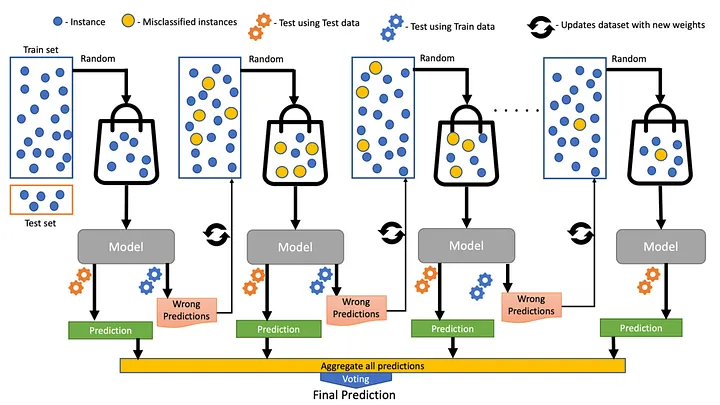
\includegraphics[width=0.82\linewidth]{Chap1/images/boosting.png}
    \caption{Principe du boosting : ajout s\'equentiel d'arbres pour corriger les erreurs du mod\`ele courant. Source : illustration p\'edagogique adapt\'ee de~\cite{verma2020xgboostillustration}.}
    \label{fig:boosting-schema}
\end{figure}
Il ressort de cette repr\'esentation que les pr\'edictions s'am\'eliorent progressivement en cumulant de petits correctifs, plut\^ot qu'en moyennant des mod\`eles parall\`eles ind\'ependants comme en bagging.

Le \textbf{gradient boosting}~\cite{friedman2001gbm} met cette id\'ee en \oe uvre en ajoutant, \`a chaque it\'eration, un arbre qui corrige les r\'esidus selon le gradient d'une fonction de perte diff\'erentiable.
On \'ecrit souvent la pr\'ediction additive sous la forme
\begin{equation}
    F_M(\mathbf{x}) = F_{M-1}(\mathbf{x}) + \eta \, h_M(\mathbf{x}),
    \label{eq:boosting}
\end{equation}
o\`u $h_M$ est un nouvel arbre entra\^in\'e sur les r\'esidus et $\eta$ un taux d'apprentissage.
Dans la pratique, le boosting construit souvent des arbres \textbf{courts} (faible profondeur) afin de corriger progressivement les erreurs sans sur-ajuster le bruit.
Le param\`etre $\eta$ (\emph{learning rate}) contr\^ole la contribution de chaque nouvel arbre : une valeur faible stabilise l'apprentissage mais exige davantage d'it\'erations.
Le nombre d'arbres, la profondeur maximale et les contraintes de r\'egularisation gouvernent ainsi le compromis entre \textbf{capacit\'e de mod\'elisation} et \textbf{g\'en\'eralisation}.

\textbf{Exemple (XGBoost et LightGBM).}
\textbf{XGBoost} (\emph{eXtreme Gradient Boosting})~\cite{chen2016xgboost} est l'une des impl\'ementations les plus utilis\'ees sur \textbf{donn\'ees tabulaires}, notamment lorsque l'on recherche un mod\`ele performant et robuste.
Son apprentissage optimise une fonction objectif compos\'ee d'un terme de perte et d'un terme de complexit\'e :
\[
\mathcal{J}^{(t)} = \sum_{i=1}^{n} l\!\left(y_i,\hat{y}_i^{(t-1)} + f_t(\mathbf{x}_i)\right) + \Omega(f_t),
\]
avec une r\'egularisation typique
\[
\Omega(f) = \gamma T + \frac{\lambda}{2}\sum_{j=1}^{T} w_j^2 + \alpha \sum_{j=1}^{T} |w_j|,
\]
o\`u $T$ est le nombre de feuilles, $w_j$ les poids des feuilles, et $(\alpha,\lambda,\gamma)$ les coefficients de p\'enalisation.
Cette formulation explicite permet de limiter la complexit\'e des arbres et de r\'eduire le surapprentissage.

En pratique, les hyperparam\`etres les plus influents sont :
\begin{itemize}
    \item \texttt{n\_estimators} : nombre d'arbres ajout\'es ;
    \item \texttt{max\_depth} : profondeur maximale des arbres ;
    \item \texttt{learning\_rate} : poids de chaque nouvel arbre ;
    \item \texttt{subsample} et \texttt{colsample\_bytree} : sous-\'echantillonnage des observations et des variables ;
    \item \texttt{reg\_alpha}, \texttt{reg\_lambda} et \texttt{gamma} : contr\^ole de la r\'egularisation.
\end{itemize}
XGBoost prend aussi en charge les valeurs manquantes en apprenant une direction de branche par d\'efaut lors des splits, et propose des impl\'ementations efficaces (\emph{histogram-based}, parall\'elisation) adapt\'ees aux volumes de donn\'ees importants.
Dans un cadre appliqu\'e, XGBoost est souvent mobilis\'e comme mod\`ele de r\'ef\'erence fort ou comme composant d'un empilement, car il combine bonne pr\'ecision, robustesse et interpr\'etabilit\'e globale (importance des variables, SHAP).

\textbf{LightGBM} (\emph{Light Gradient Boosting Machine})~\cite{ke2017lightgbm} privil\'egie une croissance des arbres \textbf{feuille par feuille} (\emph{leaf-wise}) et introduit des m\'ecanismes d'\'echantillonnage (GOSS) et de regroupement de variables (EFB) pour acc\'el\'erer l'entra\^inement sur de grands jeux de donn\'ees.




\mySubSubSection{Stacking}{}
\label{sec:stacking}

Le \textbf{stacking} (\emph{stacked generalization}) place un \textbf{m\'eta-classifieur} (ou m\'eta r\'egresseur) au-dessus de plusieurs \textbf{mod\`eles de base} de natures \'eventuellement diff\'erentes.
Chaque mod\`ele de base produit une pr\'ediction (ou une probabilit\'e) ; le m\'eta-mod\`ele apprend \`a les combiner de mani\`ere optimale, au lieu de se limiter \`a un vote fixe comme en bagging.
L'id\'ee centrale est que des mod\`eles diff\'erents capturent des \textbf{signaux compl\'ementaires} : un mod\`ele peut mieux exploiter les interactions non lin\'eaires tabulaires, un autre la structure relationnelle, un autre encore des effets locaux.
Le stacking apprend donc une \textbf{fonction de fusion} des sorties de base plut\^ot qu'une r\`egle de combinaison fix\'ee a priori.

Si l'on note $p_k(\mathbf{x})$ la sortie du $k$-i\`eme mod\`ele de base, le m\'eta-mod\`ele apprend une fonction
\[
\hat{y} = g\!\big(p_1(\mathbf{x}), p_2(\mathbf{x}), \dots, p_K(\mathbf{x})\big),
\]
o\`u $g$ peut \^etre, selon les cas, une r\'egression logistique, un arbre de d\'ecision, un gradient boosting ou un autre classifieur.
En pratique, les entr\'ees de $g$ peuvent \^etre enrichies par des variables de confiance (entropie des probabilit\'es, \'ecart entre mod\`eles, etc.).

\textbf{Exemple (m\'eta-classifieur sur sorties de bases).}
On peut par exemple empiler une for\^et al\'eatoire, un gradient boosting et un mod\`ele produisant des embeddings (graphe ou autre), puis entra\^iner un classifieur final sur les vecteurs de pr\'edictions produits par ces bases.

La figure~\ref{fig:stacking} r\'esume l'architecture hi\'erarchique du stacking.

\begin{figure}[H]
    \centering
    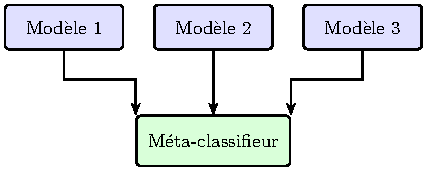
\includegraphics[width=0.78\linewidth]{Chap1/images/fig-stacking-ensemble.pdf}
    \caption{Principe du stacking : plusieurs mod\`eles de base alimentent un m\'eta-classifieur.}
    \label{fig:stacking}
\end{figure}
La figure souligne que le m\'eta-mod\`ele ne re\c{c}oit pas les variables brutes mais les sorties des apprenants de base, permettant ainsi de combiner des mod\`eles de natures diff\'erentes.

Pour \'eviter le surapprentissage, les entr\'ees du m\'eta-classifieur doivent provenir de \textbf{pr\'edictions hors \'echantillon} : les mod\`eles de base ne doivent pas avoir vu les exemples utilis\'es pour entra\^iner le m\'eta-mod\`ele.
La proc\'edure usuelle repose sur une validation crois\'ee en deux niveaux :
\begin{itemize}
    \item niveau 1 : g\'en\'erer, pour chaque observation d'entra\^inement, des pr\'edictions hors pli des mod\`eles de base ;
    \item niveau 2 : entra\^iner le m\'eta-mod\`ele sur cette matrice de m\'eta-caract\'eristiques, puis r\'eentra\^iner les mod\`eles de base sur l'ensemble d'entra\^inement.
\end{itemize}
Cette discipline m\'ethodologique est essentielle pour obtenir un gain r\'eel au test.

Le stacking est particuli\`erement utile quand la performance individuelle des mod\`eles est proche mais que leurs erreurs ne se recouvrent pas totalement.
Il peut toutefois \^etre sensible \`a la complexit\'e du m\'eta-mod\`ele et \`a la qualit\'e des pr\'edictions de base ; un protocole d'\'evaluation rigoureux reste donc indispensable.

Le tableau~\ref{tab:ensemble-comparaison} pr\'esente les trois familles d'ensembles et un exemple repr\'esentatif pour chacune ; pour les donn\'ees tabulaires de taille mod\'er\'ee, les ensembles d'arbres restent souvent tr\`es comp\'etitifs face \`a des r\'eseaux profonds g\'en\'eriques~\cite{borisov2024tabular}.

\begin{table}[h!]
    \centering
    \caption{Synth\`ese des trois familles d'ensembles et d'un exemple repr\'esentatif pour chacune.}
    \label{tab:ensemble-comparaison}
    \begin{tabular}{lp{3.2cm}p{3.2cm}p{3.5cm}}
        \hline
        Famille & Construction & Effet vis\'e & Exemple \\
        \hline
        Bagging & Parall\`ele sur tirages bootstrap & R\'eduit la variance & For\^et al\'eatoire \\
        Boosting & S\'equentielle sur les r\'esidus & R\'eduit le biais & XGBoost, LightGBM \\
        Stacking & M\'eta-mod\`ele sur les sorties des bases & Combine des mod\`eles h\'et\'erog\`enes & M\'eta-classifieur \\
        \hline
    \end{tabular}
\end{table}



\mySection{Graphes et r\'eseaux de neurones sur graphes}{}
\label{sec:graphes-gnn}

Les donn\'ees de surveillance des eaux souterraines sont souvent stock\'ees sous forme \textbf{tabulaire} (une ligne par puits, une colonne par variable).
Or, un site de pr\'el\`evement n'est pas isol\'e : il partage un contexte g\'eologique, une proximit\'e d'installations, des co-contaminants et une position g\'eographique avec d'autres sites.
Les \textbf{graphes} offrent un langage naturel pour repr\'esenter ces d\'ependances et les exploiter par apprentissage profond, en compl\'ement des mod\`eles tabulaires (for\^ets al\'eatoires, XGBoost) pr\'esent\'es en section~\ref{sec:bagging}--\ref{sec:stacking}.

\mySubSection{Repr\'esentation des donn\'ees par graphe}{}
\label{sec:graphe-basics}

Un \textbf{graphe} $G = (V, E)$ mod\'elise des entit\'es par des \textbf{n\oe uds} $v \in V$ et des liens par des \textbf{ar\^etes} $e \in E$~\cite{hamilton2017inductive}.
Chaque n\oe ud peut porter un vecteur de caract\'eristiques $\mathbf{x}_v \in \mathbb{R}^{d_v}$.
En classification de sites, on associe en g\'en\'eral \`a chaque n\oe ud \textbf{sample} (\'echantillon) une \textbf{\'etiquette} $y_v$ (par exemple contamination oui/non).

Contrairement \`a une image (grille r\'eguli\`ere) ou \`a une s\'equence (cha\^ene), un graphe autorise des connexions \textbf{irr\'eguli\`eres} : le voisinage d'un site n'est pas impos\'e par la position dans un tableau, mais par la structure relationnelle choisie.
Cette flexibilit\'e est utile lorsque l'on veut relier explicitement un puits \`a des variables de contexte (environnement, installations, qualit\'e de l'eau, regroupement g\'eographique).

On distingue :
\begin{itemize}
    \item le \textbf{graphe homog\`ene} : un seul type de n\oe ud et un seul type d'ar\^ete ;
    \item le \textbf{graphe h\'et\'erog\`ene} : plusieurs types de n\oe uds et d'ar\^etes typ\'ees, not\'ees $(s, r, t)$ pour une relation $r$ entre un n\oe ud source de type $s$ et un n\oe ud cible de type $t$.
\end{itemize}
En surveillance environnementale, l'h\'et\'erog\'en\'eit\'e refl\`ete le mod\`ele conceptuel \textbf{source, voie et r\'ecepteur} (section~\ref{sec:pfas-svr}) : sources d'activit\'e, milieux de transport, sites de mesure.


\mySubSection{R\'eseaux de neurones sur graphes}{}
\label{sec:gnn}

Les \textbf{r\'eseaux de neurones sur graphes} (GNN, \emph{Graph Neural Networks}) apprennent une \textbf{repr\'esentation vectorielle} (\emph{embedding}) pour chaque n\oe ud en diffusant l'information de proche en proche.
Le m\'ecanisme standard est le \textbf{message passing} : \`a chaque couche $\ell$, un n\oe ud agr\`ege les messages de ses voisins $\mathcal{N}(v)$ puis met \`a jour sa repr\'esentation :
\[
\mathbf{h}_v^{(\ell+1)} = \mathrm{UPDATE}\!\left(\mathbf{h}_v^{(\ell)},\, \mathrm{AGGREGATE}\big(\{\mathbf{h}_u^{(\ell)} : u \in \mathcal{N}(v)\}\big)\right).
\]

La figure~\ref{fig:message-passing} illustre ce m\'ecanisme sur un n\oe ud central et ses voisins.

\begin{figure}[H]
    \centering
    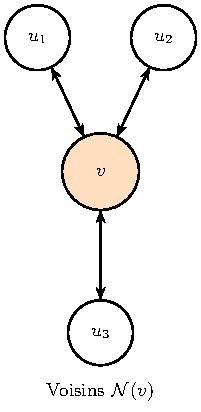
\includegraphics[width=0.55\linewidth]{Chap1/images/fig-message-passing.pdf}
    \caption{Message passing : agr\'egation des repr\'esentations des voisins $\mathcal{N}(v)$ vers le n\oe ud $v$.}
    \label{fig:message-passing}
\end{figure}
L'information locale se propage ainsi par couches successives : apr\`es $\ell$ it\'erations, $\mathbf{h}_v^{(\ell)}$ encode un voisinage \`a $\ell$ sauts~\cite{kipf2017gcn,fey2019pyg}.

Des variantes historiques incluent les \textbf{GCN} (\emph{Graph Convolutional Networks}), les \textbf{GAT} (\emph{Graph Attention Networks}) et \textbf{GraphSAGE}, qui diff\`erent par la fonction d'agr\'egation et la pond\'eration des voisins.
En pratique, ces mod\`eles sont souvent impl\'ement\'es avec des biblioth\`eques sp\'ecialis\'ees telles que \textbf{PyTorch Geometric} (PyG), qui fournit des structures de donn\'ees et des couches convolutives sur graphe~\cite{fey2019pyg}.


\mySubSection{Graphes h\'et\'erog\`enes}{}
\label{sec:graphes-heterogenes}

Un \textbf{graphe h\'et\'erog\`ene} (ou \emph{graphe typ\'e}) \'etend la d\'efinition \'el\'ementaire $G=(V,E)$ en associant un type \`a chaque n\oe ud et \`a chaque ar\^ete~\cite{hu2020hgt} :
\[
G = (V,\, E,\, \tau,\, \phi),
\]
o\`u $\tau : V \to \mathcal{T}$ est la fonction de typage des n\oe uds ($|\mathcal{T}| \geq 2$) et $\phi : E \to \mathcal{R}$ celle des ar\^etes ($|\mathcal{R}| \geq 2$).
Chaque type de n\oe ud $A \in \mathcal{T}$ dispose de son propre espace de caract\'eristiques $\mathbb{R}^{d_A}$, ce qui autorise des entit\'es de natures radicalement diff\'erentes (auteurs, articles, lieux de publication, th\`emes de recherche) \`a cohabiter dans la m\^eme structure relationnelle.

Une \textbf{m\'eta-relation} est un triplet $\langle A, r, B \rangle \in \mathcal{T} \times \mathcal{R} \times \mathcal{T}$ d\'ecrivant un lien de type $r$ entre un n\oe ud source de type $A$ et un n\oe ud cible de type $B$.
Deux n\oe uds peuvent ainsi \^etre reli\'es par des ar\^etes de s\'emantiques distinctes (co-autorat, citation, appartenance \`a un m\^eme domaine) ; le mod\`ele peut apprendre des param\`etres d'agr\'egation distincts pour chaque m\'eta-relation plut\^ot qu'un seul ensemble de param\`etres partag\'e.

Une \textbf{m\'eta-chemin} d\'esigne une s\'equence ordonn\'ee de types de n\oe uds reli\'es par des types de relations :
\[
\mathcal{P} :\ A_0 \xrightarrow{r_1} A_1 \xrightarrow{r_2} A_2 \;\cdots\; \xrightarrow{r_\ell} A_\ell.
\]
Les m\'eta-chemins capturent des d\'ependances s\'emantiques compos\'ees qui ne sont pas visibles dans le voisinage imm\'ediat.
Par exemple, dans un r\'eseau acad\'emique, le m\'eta-chemin $\texttt{Auteur} \xrightarrow{\text{\'ecrit}} \texttt{Article} \xrightarrow{\text{\'ecrit\_par}} \texttt{Auteur}$ identifie deux chercheurs ayant co-publi\'e sans qu'une ar\^ete directe entre eux soit pr\'esente dans le graphe.

Ce formalisme s'applique dans de nombreux domaines o\`u les entit\'es et leurs relations sont intrins\`equement h\'et\'erog\`enes : r\'eseaux acad\'emiques (auteurs, articles, lieux, domaines)~\cite{hu2020hgt}, graphes biom\'edicaux associant g\`enes, maladies et m\'edicaments, graphes de connaissance \`a large \'echelle, ou encore r\'eseaux de surveillance environnementale o\`u plusieurs cat\'egories d'entit\'es sont reli\'ees par des liens typ\'es.
La conception du graphe h\'et\'erog\`ene utilis\'e dans cette \'etude est d\'etaill\'ee au chapitre~3.

Contrairement aux GNN homog\`enes, les GNN h\'et\'erog\`enes doivent g\'erer simultan\'ement des espaces de caract\'eristiques de dimensions diff\'erentes selon le type de n\oe ud.
La solution usuelle est de projeter les vecteurs de chaque type dans un espace latent commun de dimension $d$ avant les op\'erations d'agr\'egation, puis de sp\'ecialiser les param\`etres d'attention selon la m\'eta-relation.
C'est pr\'ecis\'ement ce m\'ecanisme que le \textbf{HGT} (section~\ref{sec:hgt}) formalise par des matrices de cl\'e ($\mathbf{K}$), de requ\^ete ($\mathbf{Q}$) et de valeur ($\mathbf{V}$) propres \`a chaque type de n\oe ud et de relation.


\mySubSection{Heterogeneous Graph Transformer (HGT)}{}
\label{sec:hgt}

Le \textbf{Heterogeneous Graph Transformer} (HGT)~\cite{hu2020hgt} adapte le m\'ecanisme d'\textbf{attention} des transformeurs aux graphes h\'et\'erog\`enes.
Pour une m\'eta-relation $(\tau_s, \phi, \tau_t)$, les poids d'attention d\'ependent du type de n\oe ud source, du type de relation et du type de n\oe ud cible.
Chaque type dispose de projections sp\'ecifiques (matrices requ\^ete, cl\'e, valeur), ce qui permet d'apprendre des interactions diff\'erenci\'ees entre, par exemple, un lien \emph{g\'eographique} et un lien \emph{de qualit\'e de l'eau}.

Pour un message envoy\'e d'un voisin $u$ vers un n\oe ud cible $v$, l'attention peut s'\'ecrire sch\'ematiquement :
\[
\alpha_{uv} = \mathrm{softmax}\!\left(\frac{(\mathbf{K}_{\tau(u)}\,\mathbf{h}_u)^{\top}(\mathbf{Q}_{\tau(v)}\,\mathbf{h}_v)}{\sqrt{d}}\right),
\qquad
\mathbf{h}_v' = \sum_{u \in \mathcal{N}(v)} \alpha_{uv}\, \mathbf{V}_{\phi(u,v)} \mathbf{h}_u,
\]
o\`u $\mathbf{K}_{\tau(u)}$ (cl\'e, type source) et $\mathbf{Q}_{\tau(v)}$ (requ\^ete, type cible) sont des projections sp\'ecifiques au type, et $\mathbf{V}$ d\'epend du type de relation~\cite{hu2020hgt}.
Des couches \texttt{HGTConv} sont empil\'ees pour produire, en sortie, un \textbf{embedding} de dimension fixe pour chaque n\oe ud \texttt{sample}.

La figure~\ref{fig:hgt-architecture} illustre le m\'ecanisme d'attention h\'et\'erog\`ene du HGT : les n\oe uds sources projettent leurs repr\'esentations via les matrices cl\'e ($\mathbf{K}$), les n\oe uds cibles via les matrices requ\^ete ($\mathbf{Q}$), et les valeurs ($\mathbf{V}$) sont pond\'er\'ees par les scores d'attention avant agr\'egation.

\begin{figure}[htbp]
    \centering
    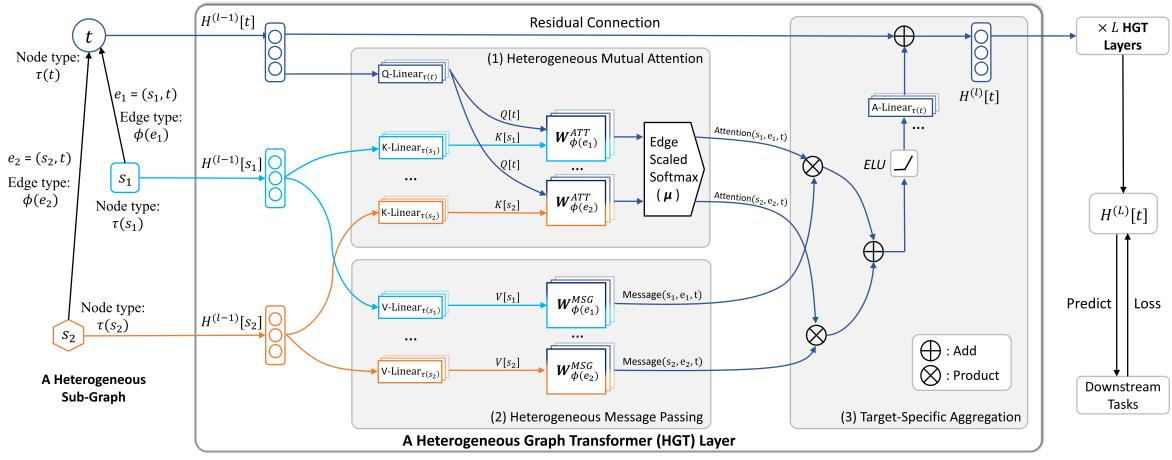
\includegraphics[width=0.90\linewidth]{Chap1/images/HGT.png}
    \caption{Architecture du Heterogeneous Graph Transformer (HGT) : attention typ\'ee par m\'eta-relation pour la propagation de l'information dans un graphe h\'et\'erog\`ene. Source : adapt\'e de~\cite{hu2020hgt}.}
    \label{fig:hgt-architecture}
\end{figure}
La figure souligne que chaque m\'eta-relation $(\tau_s, \phi, \tau_t)$ dispose de ses propres param\`etres de projection, ce qui permet au mod\`ele d'apprendre des interactions s\'emantiquement diff\'erentes selon la nature des n\oe uds et des liens connect\'es.

Cet embedding r\'esume l'information relationnelle diffus\'ee dans le graphe (contexte environnemental, proximit\'e d'installations, co-contaminants, voisinage g\'eographique).
Il peut ensuite \^etre exploit\'e de deux mani\`eres compl\'ementaires, au coeur des approches hybrides :
\begin{itemize}
    \item \textbf{Fusion par embeddings} : concat\'enation des embeddings HGT avec les variables tabulaires d'origine, puis apprentissage d'un classifieur XGBoost sur l'espace enrichi ;
    \item \textbf{Stacking} : utilisation des probabilit\'es ou embeddings HGT comme entr\'ees d'un m\'eta-classifieur, aux c\^ot\'es d'autres mod\`eles tabulaires (section~\ref{sec:stacking}).
\end{itemize}
Cette dualit\'e r\'ev\`ele un pont entre \textbf{donn\'ees relationnelles} (graphe) et \textbf{mod\`eles tabulaires} (boosting), utile lorsque la structure spatiale et contextuelle apporte un signal que les seules colonnes isol\'ees ne capturent pas enti\`erement.


\mySection{Interpr\'etabilit\'e des mod\`eles}{}
\label{sec:interpretabilite}

Un mod\`ele pr\'ecis mais opaque limite l'acceptation par les gestionnaires de l'eau et les r\'egulateurs : une d\'ecision de contr\^ole, de priorisation de campagnes ou de fermeture de puits exige une \textbf{justification} compr\'ehensible et reproductible.
En sant\'e environnementale, l'interpr\'etabilit\'e n'est plus un simple compl\'ement esth\'etique : elle conditionne la confiance des parties prenantes et la possibilit\'e de confronter les sorties algorithmiques \`a des connaissances de terrain (hydrog\'eologie, usages industriels, co-contaminants).
Cette section pr\'esente les notions n\'ecessaires pour lire les analyses men\'ees dans la contribution, en particulier l'approche \textbf{SHAP} et son d\'eploiement sur les mod\`eles tabulaires, fusionn\'es et empil\'es d\'ecrits aux sections~\ref{sec:stacking} et~\ref{sec:hgt}.


\mySubSection{Enjeux et interpr\'etabilit\'e a posteriori}{}
\label{sec:interpretabilite-enjeux}

On distingue en pratique deux familles d'approches.
L'interpr\'etabilit\'e \textbf{intrins\`eque} repose sur des mod\`eles structurellement lisibles (arbres de d\'ecision peu profonds, r\'egressions lin\'eaires avec coefficients explicites).
L'interpr\'etabilit\'e \textbf{a posteriori} (\emph{post-hoc}) applique, apr\`es entra\^inement, des m\'ethodes qui expliquent les pr\'edictions d'un mod\`ele potentiellement complexe (for\^et al\'eatoire, gradient boosting, r\'eseau sur graphe).
Les importances par impuret\'e des for\^ets al\'eatoires (section~\ref{sec:bagging}) donnent un ordre de grandeur global, mais elles ne d\'ecrivent pas la contribution \`a une pr\'ediction individuelle ni ne satisfont des axiomes de r\'epartition \'equitable entre variables corr\'el\'ees.
Les importances par permutation~\cite{breiman2001rf} corrigent partiellement ce biais en mesurant la d\'egradation de performance lorsqu'une variable est m\'elang\'ee al\'eatoirement sur l'\'echantillon de validation ; elles s'appliquent \`a tout type de mod\`ele mais restent globales, insensibles \`a la direction de l'effet et co\^uteuses \`a calculer quand le nombre de variables est \'elev\'e.

\textbf{LIME} (\emph{Local Interpretable Model-agnostic Explanations})~\cite{ribeiro2016lime} adopte une logique locale : pour chaque observation, un mod\`ele lin\'eaire interpr\'etable est ajust\'e sur des perturbations de l'entr\'ee pond\'er\'ees par leur proximit\'e au point d'int\'er\^et.
La flexibilit\'e de LIME est un atout, mais la stabilit\'e des explications d\'epend fortement du protocole d'\'echantillonnage et peut varier d'une ex\'ecution \`a l'autre, ce qui limite son usage dans des contextes r\'eglementaires exigeant la reproductibilit\'e.

L'approche \textbf{SHAP} (\emph{SHapley Additive exPlanations})~\cite{lundberg2017shap} fournit un cadre unifi\'e : chaque variable re\c{c}oit une contribution additive \`a la pr\'ediction, fond\'ee sur la th\'eorie des jeux coop\'eratifs.
Elle s'applique naturellement aux mod\`eles \`a arbres mobilis\'es dans ce m\'emoire (XGBoost, LightGBM) via l'algorithme \textbf{TreeSHAP}, et se prolonge aux espaces de features enrichis (fusion d'embeddings, m\'eta-caract\'eristiques de stacking).


\mySubSection{Valeurs de Shapley et d\'ecomposition additive}{}
\label{sec:shapley-shap}

Pour une pr\'ediction $f(\mathbf{x})$ sur un vecteur de variables $\mathbf{x} = (x_1,\ldots,x_p)$, la contribution SHAP de la variable $i$ repose sur la \textbf{valeur de Shapley} :
\begin{equation}
    \phi_i = \sum_{S \subseteq \mathcal{F} \setminus \{i\}}
    \frac{|S|!\,(|\mathcal{F}|-|S|-1)!}{|\mathcal{F}|!}
    \bigl[f(S \cup \{i\}) - f(S)\bigr],
    \label{eq:shapley}
\end{equation}
o\`u $\mathcal{F} = \{1,\ldots,p\}$ est l'ensemble des indices de variables et $f(S)$ la pr\'ediction moyenne du mod\`ele lorsque seules les variables de la coalition $S$ sont observ\'ees, les autres \'etant marginalis\'ees selon la distribution de r\'ef\'erence (souvent l'\'echantillon d'entra\^inement ou de test).

Chaque variable est vue comme un \emph{joueur} ; la coalition $S$ repr\'esente un sous-ensemble de variables disponibles pour la pr\'ediction.
Le terme $f(S \cup \{i\}) - f(S)$ mesure le \textbf{gain marginal} de $i$ lorsque $S$ est d\'ej\`a connu ; la formule~\eqref{eq:shapley} en fait la moyenne pond\'er\'ee sur toutes les coalitions, ce qui \'evite qu'une variable corr\'el\'ee monopolise tout le cr\'edit ou soit ignor\'ee selon l'ordre d'introduction.

Cette construction v\'erifie des propri\'et\'es souhaitables~\cite{lundberg2017shap} :
\begin{itemize}
    \item \textbf{Efficacit\'e} : $\sum_{i=1}^{p} \phi_i = f(\mathbf{x}) - \mathbb{E}[f(\mathbf{X})]$, o\`u $\mathbb{E}[f(\mathbf{X})]$ est la \textbf{valeur de base} (\emph{expected value}) du mod\`ele ;
    \item \textbf{Sym\'etrie} : deux variables ayant la m\^eme contribution marginale sur toute coalition re\c{c}oivent la m\^eme valeur SHAP ;
    \item \textbf{Nullit\'e} : une variable sans effet re\c{c}oit $\phi_i = 0$ ;
    \item \textbf{Additivit\'e} : pour un ensemble de mod\`eles combin\'es additivement, les contributions se somment.
\end{itemize}

La pr\'ediction s'\'ecrit ainsi sous forme additive :
\[
f(\mathbf{x}) = \phi_0 + \sum_{i=1}^{p} \phi_i,
\qquad
\phi_0 = \mathbb{E}[f(\mathbf{X})],
\]
ce qui permet de lire, pour chaque observation, quelles variables \textbf{augmentent} ou \textbf{diminuent} la sortie du mod\`ele par rapport \`a la moyenne.

Le calcul exact de l'\'equation~\eqref{eq:shapley} est exponentiel en $p$ (toutes les coalitions).
\textbf{TreeSHAP}~\cite{lundberg2017shap} exploite la structure des arbres de d\'ecision pour obtenir des valeurs SHAP \textbf{exactes} en temps polynomial pour XGBoost, LightGBM et les for\^ets al\'eatoires.
En pratique, on instancie un \texttt{TreeExplainer} sur le booster entra\^in\'e ; \`a d\'efaut, XGBoost expose aussi des \emph{pred\_contribs} (contributions par feuille) compatibles avec la m\^eme lecture additive.


\mySubSection{Analyses globale et locale}{}
\label{sec:shap-global-local}

Les sorties SHAP se lisent \`a deux \'echelles compl\'ementaires.

\paragraph{Niveau global.}
On agr\`ege typiquement les valeurs absolues $|\phi_i|$ sur un jeu d'observations (souvent l'\'echantillon de test) pour obtenir une \textbf{importance moyenne} par variable.
Le graphique en barres (\emph{bar plot}) classe les variables par ordre d\'ecroissant de cette importance.
Le graphique en nuage (\emph{beeswarm}, ou \emph{summary plot}) repr\'esente, pour chaque variable, la distribution des $\phi_i$ : la position horizontale indique l'ampleur et le signe de l'effet, la couleur le niveau de la variable (faible ou \'elev\'e).
On observe ainsi non seulement \emph{quelles} variables comptent le plus, mais aussi si une valeur \'elev\'ee de la variable pousse g\'en\'eralement vers la classe positive ou n\'egative~\cite{lundberg2017shap}.

\paragraph{Niveau local.}
Pour une observation $\mathbf{x}^{(j)}$ (un puits, un point de surveillance), les $\phi_i^{(j)}$ d\'ecrivent la pr\'ediction individuelle.
Le \textbf{graphique de force} (\emph{force plot}) aligne les contributions positives (vers la classe \emph{contamin\'e}) et n\'egatives (vers la classe \emph{non contamin\'e}) autour de la valeur de base $\phi_0$.
Un barplot local des $| \phi_i^{(j)} |$ les plus \'elev\'es offre une vue synth\'etique pour un cas d'\'etude.
Ces vues sont utiles pour expliquer \`a un expert pourquoi un site pr\'ecis a \'et\'e class\'e \`a risque, au-del\`a d'un score global.

\paragraph{Relations non lin\'eaires.}
Les \textbf{graphiques de d\'ependance} (\emph{dependence plots}) repr\'esentent, pour une variable $i$, la valeur de $x_i$ en abscisse et $\phi_i$ en ordonn\'ee.
Ils mettent en \'evidence des effets \`a seuil, des saturations ou des interactions (en colorant les points selon une deuxi\`eme variable corr\'el\'ee).
Pour des classifieurs par arbres, on peut y v\'erifier que le mod\`ele reproduit des comportements plausibles (par exemple une influence accrue de la proximit\'e d'une source industrielle au-del\`a d'un certain rayon), sans confondre cette coh\'erence avec une preuve causale.


\mySubSection{Limites et recul \'epist\'emologique}{}
\label{sec:interpretabilite-limites}

Une variable importante au sens SHAP (proximit\'e d'une installation, co-contaminant, embedding li\'e \`a un cluster g\'eographique) signale une \textbf{association statistique} apprise par le mod\`ele, pas un m\'ecanisme physique d\'emonstr\'e.
Les variables corr\'el\'ees se partagent le cr\'edit : l'ordre d'importance peut varier selon l'\'echantillon et la distribution de r\'ef\'erence.
Les explications portent sur le \textbf{mod\`ele entra\^in\'e} et le jeu de donn\'ees consid\'er\'e ; un r\'eentra\^inement ou un changement de protocole (par exemple passage au mode confirmatoire avec concentrations PFAS) peut modifier les profils SHAP m\^eme si les tendances physiques demeurent qualitatives.

Pour le HGT, la partie du signal port\'ee par la \textbf{topologie} du graphe (chemins entre \texttt{facility}, \texttt{env}, \texttt{sample}) n'est pas enti\`erement d\'epli\'ee dans les graphiques tabulaires ou d'embeddings.
Enfin, l'usage op\'erationnel suppose une \textbf{lecture conjointe} avec des hydrog\'eologues et des toxicologues : l'outil priorise et explique, la d\'ecision publique reste argument\'ee au-del\`a du seul score algorithmique.


\mySection{Synth\`ese}{}
\label{sec:synthese-chap1}

Ce chapitre a introduit, de mani\`ere autonome et progressive, les concepts mobilis\'es dans la suite du m\'emoire.
Les \textbf{PFAS} ont \'et\'e pr\'esent\'es comme polluants persistants, soumis \`a un encadrement r\'eglementaire de plus en plus strict.
Les paradigmes de l'\textbf{apprentissage automatique} (supervis\'e, non supervis\'e, semi-supervis\'e et par renforcement), les m\'ethodes d'ensemble par \textbf{bagging} (for\^et al\'eatoire), \textbf{boosting} (XGBoost, LightGBM) et \textbf{stacking} (m\'eta-classifieur) constituent le socle des m\'ethodes pr\'edictives en donn\'ees tabulaires.
Les \textbf{graphes h\'et\'erog\`enes}, les GNN, le \textbf{HGT} et les sch\'emas de fusion ou de stacking entre embeddings graphiques et mod\`eles tabulaires, pr\'eparent la lecture des approches hybrides d\'evelopp\'ees dans la suite du m\'emoire.
Enfin, \textbf{SHAP} et TreeSHAP (analyses globale et locale, graphiques de d\'ependance) permettent d'expliquer les mod\`eles tabulaires, la fusion embeddings--XGBoost, le stacking sur m\'eta-caract\'eristiques et, partiellement, le HGT par sensibilit\'e au gradient ; cette interpr\'etabilit\'e conditionne une utilisation responsable en sant\'e environnementale, sous r\'eserve d'un recul sur la causalit\'e.


	\myChapter{\'Etat de l'art sur la pr\'ediction des contaminants \'emergents de l'eau par intelligence artificielle}{\'Etat de l'art}
\label{chap:etat-art}
\myMiniToc{section}{Sommaire}

% =========================================================
\mySection{Introduction}{}
\label{sec:intro-chap2}
% =========================================================

La surveillance des PFAS dans les eaux souterraines constitue un d\'efi analytique et \'economique~: une analyse par chromatographie liquide coupl\'ee \`a la spectrom\'etrie de masse tandem co\^ute plusieurs centaines d'euros par \'echantillon, alors que les seuils r\'eglementaires se durcissent (4~ng/L pour le PFOA et le PFOS depuis 2023 aux \'Etats-Unis~\cite{epa2023npdwr}, 0,5~$\mu$g/L pour la somme des PFAS dans la directive europ\'eenne 2020/2184~\cite{eu2020drinkingwater}).
Un contr\^ole exhaustif du parc de puits \'etant hors de port\'ee de la plupart des gestionnaires, les m\'ethodes d'intelligence artificielle se sont impos\'ees comme outils de priorisation~: orienter les campagnes vers les sites \`a plus forte probabilit\'e de d\'epassement, \`a partir d'informations contextuelles disponibles sans analyse PFAS pr\'ealable.
Les enjeux sanitaires, la chimie des PFAS et les fondements algorithmiques mobilis\'es ayant \'et\'e d\'etaill\'es au chapitre~\ref{chap:generalites}, ce chapitre se concentre sur leur application \`a la surveillance.

Depuis la d\'ecennie 2010, deux g\'en\'erations de m\'ethodes sont bien document\'ees, une troisi\`eme \'etant en cours de constitution.
La premi\`ere repose sur des mod\`eles probabilistes et tabulaires (r\'eseaux bay\'esiens, for\^ets al\'eatoires, gradient boosting) traitant chaque puits comme un vecteur de descripteurs ind\'ependants.
La deuxi\`eme introduit des architectures plus complexes~: d'abord des r\'eseaux de neurones sur donn\'ees mol\'eculaires (QSAR), puis des cha\^ines de classifieurs semi-supervis\'ees pr\'edisant simultan\'ement plusieurs dizaines d'analytes.
La troisi\`eme, encore embryonnaire dans la litt\'erature PFAS publi\'ee, mobilise les graphes h\'et\'erog\`enes pour encoder explicitement la topologie du r\'eseau de surveillance~; aucune \'etude ne l'a syst\'ematiquement valid\'ee sur ce type de donn\'ees.

Ce chapitre examine ces deux g\'en\'erations et la direction \'emergente de mani\`ere structur\'ee~: le cadre conceptuel de la revue (section~\ref{sec:chap2-cadre}), dont la distinction mode pr\'edictif/confirmatoire (section~\ref{sec:chap2-modes})~; les m\'ethodes tabulaires, probabilistes, d'ensemble et d'attribution de sources (section~\ref{sec:chap2-tabulaire})~; les architectures profondes et relationnelles (section~\ref{sec:chap2-deep})~; une discussion transversale (section~\ref{sec:chap2-discussion}) assortie des lacunes structurelles (section~\ref{sec:chap2-lacunes})~; enfin une synth\`ese (section~\ref{sec:synthese-chap2}).


% =========================================================
\mySection{Cadre conceptuel de la revue}{}
\label{sec:chap2-cadre}
% =========================================================

Avant d'examiner les travaux, cinq \'el\'ements conceptuels propres \`a cette revue doivent \^etre pos\'es.
Le premier est la formalisation du probl\`eme de pr\'ediction ML sur donn\'ees PFAS.
Le deuxi\`eme relie la s\'election des variables contextuelles aux m\'ecanismes physico-chimiques de transport des PFAS, fondement commun \`a toutes les \'etudes examin\'ees.
Le troisi\`eme et le quatri\`eme \'etablissent le socle m\'etrique commun (m\'etriques d'\'evaluation, gestion du d\'es\'equilibre de classes) qui sert de r\'ef\'erence \`a toutes les comparaisons inter-\'etudes.
Le cinqui\`eme, et le plus fondamental, est la distinction entre mode pr\'edictif et mode confirmatoire~: mal comprise, elle conduit \`a des comparaisons de performance trompeuses entre \'etudes.


\mySubSection{Formalisation du probl\`eme de pr\'ediction PFAS par apprentissage automatique}{}
\label{sec:chap2-formalisation}

La pr\'ediction du statut de contamination d'un puits par apprentissage automatique revient \`a estimer une fonction $g : \mathcal{X} \rightarrow \mathcal{Y}$ associant \`a chaque puits, d\'ecrit par un vecteur de variables $\mathbf{x} \in \mathcal{X}$, une cible $y \in \mathcal{Y}$.
Le vecteur $\mathbf{x}$ rassemble les descripteurs disponibles (g\'eologie, hydrologie, proximit\'e aux sources, qualit\'e g\'en\'erale de l'eau)~; sa composition, avec ou sans concentrations PFAS mesur\'ees, d\'etermine le r\'egime d'\'evaluation discut\'e en section~\ref{sec:chap2-modes}.
La fonction $g$ est ajust\'ee sur un jeu d'entra\^inement \'etiquet\'e en minimisant une fonction de perte, puis \'evalu\'ee sur des donn\'ees non vues (section~\ref{sec:ml-supervise}).

Les travaux examin\'es se distinguent par la nature de la cible $\mathcal{Y}$, qui commande le choix des m\'ethodes et des m\'etriques.
\begin{itemize}
    \item \emph{Classification binaire} ($y \in \{0,1\}$)~: pr\'esence ou absence d'un analyte, ou d\'epassement d'un seuil r\'eglementaire. C'est la formulation la plus r\'epandue (George et Dixit, Tokranov, Li et MacDonald Gibson, ainsi que le criblage total de Dong et al.).
    \item \emph{Classification multi-\'etiquettes} ($\mathbf{y} \in \{0,1\}^L$, $L$ analytes)~: pr\'ediction simultan\'ee de plusieurs dizaines d'analytes. Absente du cadre multiclasse classique pr\'esent\'e au chapitre~\ref{chap:generalites}, elle est propre \`a la litt\'erature PFAS~\cite{dong2024pfas} et conditionne le choix des architectures pr\'esent\'ees en section~\ref{sec:chap2-semisup}.
    \item \emph{Cartographie de vuln\'erabilit\'e} ($y$ continu ou ordinal)~: production d'un score de risque r\'egional ou national plut\^ot que d'une \'etiquette par puits (Hu et al., McMahon et al.).
\end{itemize}

Deux propri\'et\'es traversent ces formulations.
D'une part, la cible binaire d\'epend d'un seuil qui a \'evolu\'e avec la r\'eglementation, ce qui complique la comparaison directe des performances entre \'etudes anciennes et r\'ecentes (section~\ref{sec:chap2-modes}).
D'autre part, le d\'es\'equilibre structurel de classes (section~\ref{sec:chap2-desequilibre}, avec SMOTE~\cite{chawla2002smote} et ADASYN~\cite{he2008adasyn}) est particuli\`erement marqu\'e dans les corpus PFAS, le rapport entre classe minoritaire et classe majoritaire s'\'etalant de 1/10 \`a 1/50~\cite{dong2024pfas}~; le score F1 (section~\ref{sec:chap2-metriques}) sert d'indicateur de r\'ef\'erence, compl\'et\'e par la ROC-AUC pour les comparaisons inter-\'etudes.

\mySubSection{M\'ecanismes de transport des PFAS et pertinence des variables contextuelles}{}
\label{sec:chap2-transport}

La s\'election des variables contextuelles dans les mod\`eles ML de pr\'ediction des PFAS n'est pas arbitraire~: elle d\'ecoule directement des m\'ecanismes physico-chimiques qui gouvernent le devenir et le transport des PFAS en milieu souterrain.
Trois processus principaux, d\'ecrits par Guelfo et al.~\cite{guelfo2021pfas} dans une revue exhaustive de l'\'etat de la science, conditionnent la distribution spatiale des concentrations observ\'ees.

\paragraph{Advection et att\'enuation en fonction de la distance.}
Les PFAS se d\'eplacent principalement par advection avec le flux d'eau souterraine, suivant les lignes d'\'ecoulement depuis les zones de recharge vers les zones de d\'echarge.
Prevedouros et al.~\cite{prevedouros2006pfas} montrent que les concentrations de PFCAs d\'ecroissent avec la distance aux sources ponctuelles~: la proximit\'e \`a une installation fluorochimique, une base militaire (usage de mousses AFFF) ou une station d'\'epuration constitue donc un proxy du flux de contamination advectif.
C'est ce constat m\'ecaniste qui fonde l'utilisation syst\'ematique, dans toutes les \'etudes examin\'ees, du nombre d'installations \`a 1, 3, 10 et 50~km comme variables pr\'edictives.

\paragraph{R\'etention sur la matrice solide.}
Brusseau et al.~\cite{brusseau2019pfas} \'etablissent un mod\`ele de r\'etention complet montrant que les PFAS se sorbent sur la mati\`ere organique du sol et sur les interfaces air-eau des zones vadoses~: la granulom\'etrie (proportion d'argiles, de limons, uniformit\'e de la distribution), la teneur en mati\`ere organique et la profondeur de la nappe modulent fortement la mobilit\'e des diff\'erentes familles de PFAS.
Les compos\'es \`a longue cha\^ine (PFOS, PFOA) se retiennent davantage que les compos\'es \`a cha\^ine courte (PFBS, PFPeA), plus mobiles mais aussi plus difficiles \`a \'eliminer.
Ce m\'ecanisme justifie l'inclusion de descripteurs de sol (granulom\'etrie, teneur en argile, ratio eau-argile) dans les vecteurs de features des mod\`eles tabulaires.

\paragraph{D\'eposition atmosph\'erique.}
Les PFAS volatils ou semi-volatils (fluorot\'elom\`eres, sulfonamides) sont \'emis dans l'atmosph\`ere par les installations industrielles, transport\'es sur des distances pouvant d\'epasser 50~km et d\'epos\'es par les pr\'ecipitations~\cite{guelfo2021pfas}.
Ce vecteur de contamination diffus et longue port\'ee explique pourquoi les variables m\'et\'eorologiques (humidit\'e, pr\'ecipitations, qualit\'e de l'air~: PM$_{2,5}$, NO$_2$) figurent parmi les pr\'edicteurs importants identifi\'es par Dong et al.~\cite{dong2024pfas}, alors qu'elles ne sont pas directement li\'ees aux sources ponctuelles locales.

\paragraph{Cons\'equences pour la mod\'elisation par graphes.}
L'advection cr\'ee une d\'ependance spatiale structurelle entre puits~: deux puits situ\'es en aval d'une m\^eme source partagent un contexte de contamination commun qui ne peut pas \^etre captur\'e par des vecteurs ind\'ependants.
Cette d\'ependance est directionnelle (orient\'ee par le sens de l'\'ecoulement) et h\'et\'erog\`ene (fonction de l'intensit\'e du flux, de la lithologie, de la proximit\'e \`a la source).
Les graphes h\'et\'erog\`enes, et en particulier le Heterogeneous Graph Transformer~\cite{hu2020hgt}, sont con\c{c}us pour encoder cette topologie~: des n\oe uds de types distincts (puits de surveillance, installations sources, clusters g\'eographiques) sont reli\'es par des ar\^etes typ\'ees repr\'esentant la proximit\'e aux sources et le voisinage spatial, le long desquelles l'information de contamination se propage.
Cette justification m\'ecaniste fonde l'int\'er\^et des architectures relationnelles, discut\'ees comme direction \'emergente dans la lacune~L1 (section~\ref{sec:chap2-lacunes})~: la topologie d'\'ecoulement y est encod\'ee explicitement plut\^ot que d\'eduite de variables ind\'ependantes.


\mySubSection{M\'etriques d'\'evaluation des classifieurs de contamination PFAS}{}
\label{sec:chap2-metriques}

La comparaison des m\'ethodes exig\'ee par la revue n\'ecessite un socle m\'etrique commun, d'autant que les \'etudes examin\'ees ne rapportent pas toutes les m\^emes indicateurs.
Cette section fixe les d\'efinitions retenues pour la classification binaire (pr\'esence/absence d'un PFAS, d\'epassement d'un seuil r\'eglementaire), puis pr\'ecise le passage au cas multi-\'etiquettes~; Sokolova et Lapalme~\cite{sokolova2009metrics} en proposent l'analyse syst\'ematique dont nous reprenons l'ossature.
Toutes les m\'etriques d\'erivent de la \textbf{matrice de confusion} (tableau~\ref{tab:confusion}), qui recense quatre effectifs en confrontant les pr\'edictions \`a la v\'erit\'e terrain~: vrais positifs (VP), vrais n\'egatifs (VN), faux positifs (FP) et faux n\'egatifs (FN).

\begin{table}[H]
    \centering
    \caption{Matrice de confusion pour une classification binaire (classe positive~= site contamin\'e).}
    \label{tab:confusion}
    \begin{tabular}{lcc}
        \hline
        & Pr\'edit 0 & Pr\'edit 1 \\
        \hline
        R\'eel 0 & Vrai n\'egatif (VN) & Faux positif (FP) \\
        R\'eel 1 & Faux n\'egatif (FN) & Vrai positif (VP) \\
        \hline
    \end{tabular}
\end{table}

Le choix de l'indicateur n'est pas neutre en surveillance environnementale~: un faux n\'egatif (site contamin\'e non d\'etect\'e) expose une population, l\`a o\`u un faux positif (pr\'el\`evement inutile) n'entra\^ine qu'un co\^ut analytique.
Les m\'etriques sensibles aux faux n\'egatifs sont donc privil\'egi\'ees.

\paragraph{Exactitude.}
L'exactitude $\mathrm{Acc} = (VP+VN)/(VP+VN+FP+FN)$ mesure la proportion de pr\'edictions correctes.
Sous un fort d\'es\'equilibre de classes (section~\ref{sec:chap2-desequilibre}), elle devient trompeuse~: un classifieur pr\'edisant toujours la classe majoritaire atteint une exactitude proche de 1 sans d\'etecter le moindre site contamin\'e.

\paragraph{Pr\'ecision, rappel et sp\'ecificit\'e.}
Trois quantit\'es se lisent directement dans la matrice~:
\begin{equation}
    \text{Pr\'ecision} = \frac{VP}{VP + FP}, \qquad
    \text{Rappel} = \frac{VP}{VP + FN}, \qquad
    \text{Sp\'ecificit\'e} = \frac{VN}{VN + FP}.
    \label{eq:precision-rappel}
\end{equation}
La pr\'ecision indique, parmi les sites signal\'es contamin\'es, la part qui l'est r\'eellement.
Le rappel (ou sensibilit\'e) indique, parmi les sites r\'eellement contamin\'es, la part d\'etect\'ee~; en priorisation PFAS, il prime, puisque manquer un site pollu\'e est l'erreur la plus co\^uteuse.
La sp\'ecificit\'e indique, parmi les sites r\'eellement non contamin\'es, la part correctement \'ecart\'ee (taux de vrais n\'egatifs).
Son compl\'ement $1 - \text{Sp\'ecificit\'e}$, le taux de faux positifs, constitue l'abscisse de la courbe ROC.

\paragraph{Score F1 et $F_\beta$.}
Le score F1, moyenne harmonique de la pr\'ecision et du rappel, condense ces deux quantit\'es~:
\begin{equation}
    F_1 = 2 \cdot \frac{\text{Pr\'ecision} \times \text{Rappel}}{\text{Pr\'ecision} + \text{Rappel}}.
    \label{eq:f1}
\end{equation}
Sa g\'en\'eralisation $F_\beta = (1+\beta^2)\,\dfrac{\text{Pr\'ecision} \cdot \text{Rappel}}{\beta^2\,\text{Pr\'ecision} + \text{Rappel}}$ pond\`ere le rappel par un facteur $\beta$~; choisir $\beta > 1$ p\'enalise davantage les faux n\'egatifs, conform\'ement \`a la logique de surveillance.
La moyenne harmonique chute d\`es que la pr\'ecision ou le rappel est faible, ce qui rend le F1 plus exigeant que l'exactitude sous d\'es\'equilibre~\cite{sokolova2009metrics}.

\paragraph{Coefficient de corr\'elation de Matthews.}
Le coefficient de Matthews (MCC) combine les quatre cases de la matrice~:
\begin{equation}
    \mathrm{MCC} = \frac{VP \cdot VN - FP \cdot FN}{\sqrt{(VP+FP)(VP+FN)(VN+FP)(VN+FN)}}.
    \label{eq:mcc}
\end{equation}
Born\'e entre $-1$ et $+1$, il n'est \'elev\'e que si le classifieur r\'eussit simultan\'ement sur les deux classes.
Chicco et Jurman~\cite{chicco2020mcc} montrent qu'il reste plus fiable que le F1 et l'exactitude sous fort d\'es\'equilibre, car aucune classe ne peut \`a elle seule le gonfler.

\paragraph{Courbes ROC et pr\'ecision-rappel.}
La courbe ROC trace le taux de vrais positifs contre le taux de faux positifs \`a mesure que varie le seuil de d\'ecision~; son aire (\textbf{ROC-AUC}) quantifie la s\'eparabilit\'e des classes ind\'ependamment du seuil op\'erationnel~\cite{fawcett2006roc}.
Sous d\'es\'equilibre marqu\'e, cette aire peut para\^itre optimiste~; la courbe pr\'ecision-rappel et son aire (PR-AUC) refl\`etent alors plus fid\`element la performance sur la classe positive rare~\cite{davis2006prroc,saito2015prc}.

\paragraph{Choix retenu pour la revue.}
Le F1 sert d'indicateur de r\'ef\'erence pour les comparaisons inter-\'etudes, compl\'et\'e par la ROC-AUC lorsqu'elle est rapport\'ee.
En classification multi-\'etiquettes ($L$ analytes), le \textbf{F1 macro}, moyenne uniforme sur les $L$ analytes, est privil\'egi\'e~: il accorde le m\^eme poids \`a chaque analyte et \'evite de masquer les mauvaises performances sur les compos\'es rares, contrairement au F1 micro que dominent les analytes fr\'equents~\cite{sokolova2009metrics}.


\mySubSection{D\'es\'equilibre de classes et r\'e\'echantillonnage synth\'etique}{}
\label{sec:chap2-desequilibre}

Dans les corpus de surveillance PFAS, la classe positive (d\'etection ou d\'epassement de seuil) est structurellement minoritaire~: le rapport entre classe minoritaire et classe majoritaire peut atteindre 1/10 \`a 1/50 selon les analytes et la r\'egion~\cite{dong2024pfas,george2021pfas}.
Un classifieur entra\^in\'e sans correction tend alors \`a ignorer la classe positive pour maximiser l'exactitude globale, comportement inacceptable en surveillance sanitaire o\`u c'est pr\'ecis\'ement cette classe qui importe.
He et Garcia~\cite{he2009imbalanced} distinguent quatre familles de r\'eponses, souvent combin\'ees.

\paragraph{R\'e\'echantillonnage.}
La premi\`ere agit sur la distribution du jeu d'entra\^inement, par sous-\'echantillonnage de la classe majoritaire ou sur-\'echantillonnage de la classe minoritaire.
Le sur-\'echantillonnage al\'eatoire duplique des exemples existants, au risque du surapprentissage~; SMOTE et ADASYN, dominants dans la litt\'erature PFAS, g\'en\`erent au contraire des exemples synth\'etiques.
\textbf{SMOTE} (\emph{Synthetic Minority Over-sampling Technique})~\cite{chawla2002smote} interpole lin\'eairement entre un exemple $\mathbf{x}_i$ et l'un de ses $k$ plus proches voisins minoritaires~:
\begin{equation}
    \mathbf{x}_{\mathrm{new}} = \mathbf{x}_i + \lambda\,(\mathbf{x}_j - \mathbf{x}_i), \quad \lambda \sim \mathcal{U}(0,1).
    \label{eq:smote}
\end{equation}
\textbf{ADASYN} (\emph{Adaptive Synthetic Sampling})~\cite{he2008adasyn} concentre la g\'en\'eration pr\`es de la fronti\`ere de d\'ecision~: le nombre d'exemples allou\'e \`a chaque $\mathbf{x}_i$ cro\^it avec la fraction $r_i = \Delta_i/k$ de ses $k$ voisins appartenant \`a la classe majoritaire.
Cette focalisation adaptative est pertinente lorsque les sites contamin\'es sont spatialement dispers\'es dans un corpus h\'et\'erog\`ene, comme dans les \'etudes californiennes \`a grande \'echelle.

\paragraph{Pond\'eration du co\^ut.}
La deuxi\`eme famille conserve la distribution mais p\'enalise davantage les erreurs sur la classe minoritaire, en pond\'erant la fonction de perte par l'inverse de la fr\'equence des classes.
Native dans la plupart des impl\'ementations d'arbres d'ensemble via un param\`etre de poids de classe, elle \'evite la cr\'eation d'exemples artificiels.

\paragraph{Ajustement du seuil et m\'etriques adapt\'ees.}
La troisi\`eme famille d\'eplace le seuil de d\'ecision (par d\'efaut 0,5) vers une valeur qui maximise le rappel ou le F1 sur un jeu de validation.
La quatri\`eme, transversale, \'evalue le mod\`ele avec des m\'etriques robustes au d\'es\'equilibre plut\^ot qu'avec l'exactitude (section~\ref{sec:chap2-metriques}).

\paragraph{R\`egle m\'ethodologique commune.}
Quelle que soit la technique, le r\'e\'echantillonnage ne s'applique qu'au \textbf{jeu d'entra\^inement}~; les jeux de validation et de test conservent la distribution r\'eelle des classes, faute de quoi les m\'etriques sont artificiellement gonfl\'ees.
Cette r\`egle est appliqu\'ee dans tous les travaux examin\'es~; son non-respect est signal\'e explicitement dans les limites.


\mySubSection{Mode pr\'edictif et mode confirmatoire}{}
\label{sec:chap2-modes}

Pour comparer les travaux examin\'es sur une base homog\`ene, nous distinguons deux r\'egimes d'\'evaluation selon un crit\`ere unique~: la pr\'esence ou l'absence, dans le vecteur de features, de concentrations PFAS mesur\'ees pour le puits \'evalu\'e.

Le \textbf{mode confirmatoire} d\'esigne la configuration o\`u ce vecteur comprend des concentrations PFAS mesur\'ees (partielles ou compl\`etes) et o\`u la variable cible est elle-m\^eme d\'eriv\'ee de ces mesures~: $\mathbb{1}[\texttt{PFAS\_total} > 70\text{ ng/L}]$ en r\'ef\'erence \`a l'avis sanitaire EPA 2016~\cite{epa2016pfas}.
Ce seuil de 70~ng/L, depuis abaiss\'e \`a 4~ng/L~\cite{epa2023npdwr}, demeure la r\'ef\'erence de la quasi-totalit\'e des travaux examin\'es, ce qui complique leur comparaison avec les \'etudes les plus r\'ecentes.
La configuration cr\'ee une \textbf{circularit\'e}~: les entr\'ees contiennent l'information qui d\'etermine l'\'etiquette, de sorte que les performances publi\'ees (F1 sup\'erieur \`a 0,96) ne refl\`etent pas ce que le mod\`ele ferait sur un puits jamais analys\'e.
Cette circularit\'e est le seul crit\`ere du mode confirmatoire~: la distinction ne porte donc que sur les t\^aches dont la cible est un statut de contamination d\'eriv\'e de concentrations PFAS, et ne s'applique pas aux t\^aches dont la cible est de nature diff\'erente, telles que l'attribution de sources ou la pr\'ediction de bioactivit\'e mol\'eculaire.

Le \textbf{mode pr\'edictif} correspond au sc\'enario op\'erationnellement pertinent~: classer un puits avant tout pr\'el\`evement PFAS, sur la seule base d'informations contextuelles disponibles a priori (g\'eologie, hydrologie, qualit\'e g\'en\'erale de l'eau, proximit\'e aux sources anthropiques, coordonn\'ees g\'eographiques).
Formellement, si $\mathbf{x}_c$ est le vecteur de variables contextuelles et $\mathbf{x}_p = (\tilde{c}_1, \ldots, \tilde{c}_K)$ les concentrations PFAS mesur\'ees~:
\begin{align}
    \text{Mode pr\'edictif}~: & \quad \hat{y} = g(\mathbf{x}_c), \label{eq:mode-pred} \\
    \text{Mode confirmatoire}~: & \quad \hat{y} = g(\mathbf{x}_c, \mathbf{x}_p). \label{eq:mode-conf}
\end{align}
Les deux modes r\'epondent \`a des questions m\'etiers distinctes~: le mode pr\'edictif (\guillemotleft{}~Dois-je envoyer un pr\'eleveur ?~\guillemotright{}) pr\'ec\`ede l'analyse~; le mode confirmatoire (\guillemotleft{}~Ce profil partiel indique-t-il un d\'epassement global ?~\guillemotright{}) compl\`ete un laboratoire partiellement inform\'e.
C'est le mode pr\'edictif qui d\'etermine la valeur r\'eelle d'un outil d'aide \`a la d\'ecision pour les gestionnaires de r\'eseaux.

Cette cl\'e de lecture est appliqu\'ee syst\'ematiquement \`a chaque travail examin\'e dans les sections suivantes.


% =========================================================
\mySection{Mod\`eles tabulaires pour la pr\'ediction des PFAS}{}
\label{sec:chap2-tabulaire}
% =========================================================

Les m\'ethodes tabulaires constituent le fondement de la litt\'erature pr\'edictive sur les PFAS.
Elles traitent chaque puits comme un vecteur de variables contextuelles dont la pertinence repose sur les m\'ecanismes physico-chimiques de transport des PFAS en aquif\`ere (section~\ref{sec:chap2-transport}).
Leur avantage principal est la compatibilit\'e directe avec les bases de surveillance environnementale structur\'ees en tableaux, sans recours \`a des architectures graphiques ou \`a des mod\`eles de transport hydrog\'eologique.
Leur limite structurelle est l'hypoth\`ese d'ind\'ependance des observations~: la topologie du r\'eseau de surveillance et les liens de voisinage entre puits ne sont pas exploit\'es.


\mySubSection{Approches probabilistes et cartographie pr\'ecoce de la vuln\'erabilit\'e}{}
\label{sec:chap2-bayes}

Ce premier groupe rassemble les travaux pionniers visant \`a caract\'eriser la vuln\'erabilit\'e des aquif\`eres \`a partir de proxies contextuels, avant l'usage syst\'ematique des m\'ethodes d'ensemble pour la priorisation op\'erationnelle (section~\ref{sec:chap2-ensemble}).
Les r\'eseaux bay\'esiens (graphe orient\'e acyclique, DAG) y occupent une place centrale~: ils se distinguent des m\'ethodes discriminantes classiques par leur capacit\'e \`a repr\'esenter des d\'ependances conditionnelles non monotones et \`a inf\'erer avec des donn\'ees manquantes~; pour une variable cible $Y$ et un ensemble d'observations $\mathbf{e}$, la distribution a posteriori $P(Y \mid \mathbf{e})$ est calcul\'ee en marginalisant les variables non observ\'ees via la factorisation de Markov du DAG.
Cette propri\'et\'e est d\'ecisive en surveillance des PFAS, o\`u les jeux de donn\'ees sont structurellement incomplets (valeurs censur\'ees, campagnes h\'et\'erog\`enes).
Deux travaux non bay\'esiens (McMahon et al., Hu et al.) sont rattach\'es \`a ce groupe car ils partagent le m\^eme objectif de cartographie pr\'ecoce de la vuln\'erabilit\'e r\'egionale ou nationale, distinct de la priorisation par classifieur d'ensemble.


\mySubSubSection{Travaux de Li et MacDonald Gibson (2022)}{}
\label{sec:art-li2022}

\textbf{Probl\`eme.}
Li et MacDonald Gibson~\cite{li2022pfas} cherchent \`a pr\'edire la pr\'esence des PFAS \`a cha\^ine courte (PFBS, PFBA, PFPeA et leurs pr\'ecurseurs fluorot\'elom\`eres) dans les eaux souterraines du Minnesota.
Ces compos\'es, substituts industriels aux PFAS \`a longue cha\^ine progressivement interdits, sont plus hydrophiles, plus mobiles en phase aqueuse et moins fr\'equemment mesur\'es dans les bases historiques, ce qui limite les approches purement supervis\'ees.

\textbf{M\'ethodologie.}
Les auteurs agr\`egent les donn\'ees du programme de surveillance du Minnesota, recodent les valeurs sous le seuil de d\'etection \`a LD/2 et standardisent 88 variables contextuelles couvrant~: proximit\'e aux sources industrielles (distance aux usines 3M de Cottage Grove et Oakdale), caract\'eristiques hydrog\'eologiques r\'egionales, occupation du sol et co-contaminants inorganiques.
La structure du DAG est apprise automatiquement par Hill Climbing avec score BIC.

\textbf{R\'esultats.}
Les ROC-AUC d\'epassent 0,96 pour les compos\'es les mieux repr\'esent\'es (PFOS, PFOA, PFHxS) et sont de l'ordre de 0,78 \`a 0,82 pour les compos\'es \`a cha\^ine courte.
Les ar\^etes les plus fortes du DAG relient le statut de contamination PFAS aux variables de proximit\'e industrielle, relation m\'edi\'ee par les zones humides (bassins de r\'etention des compos\'es PFAS transport\'es par ruissellement).

\textbf{Limites.}
Le mod\`ele est entra\^in\'e et valid\'e exclusivement sur le Minnesota (transf\'erabilit\'e non valid\'ee).
Le r\'eseau bay\'esien inf\`ere la cible en marginalisant les variables non observ\'ees~; lorsque des mesures PFAS partielles figurent parmi les n\oe uds observ\'es, leur contribution \`a la pr\'ediction reste difficile \`a isoler sans protocole de division strict par site.


\mySubSubSection{Travaux de McMahon et al.\ (2022)}{}
\label{sec:art-mcmahon2022}

\textbf{Probl\`eme.}
McMahon et al.~\cite{mcmahon2022pfas} cherchent \`a caract\'eriser la distribution spatiale des concentrations PFAS dans les eaux souterraines potables de l'est des \'Etats-Unis \`a partir de proxies g\'eochimiques, en s'affranchissant de mesures PFAS cibl\'ees syst\'ematiques.

\textbf{M\'ethodologie.}
Les auteurs mobilisent des arbres de r\'egression boost\'es (BRT, variante de gradient boosting, section~\ref{sec:boosting}) sur un corpus de plusieurs centaines d'\'echantillons g\'eor\'ef\'erenc\'es.
Les pr\'edicteurs incluent la concentration en tritium (\textsuperscript{3}H), le carbone organique dissous (COD), la pr\'esence de solvants chlor\'es volatils (TCE, PCE) et divers indicateurs hydrog\'eologiques r\'egionaux.

\textbf{R\'esultats (approche descriptive).}
Le tritium, indicateur d'une recharge r\'ecente, est le pr\'edicteur le plus fortement associ\'e aux concentrations PFAS \'elev\'ees~: r\'esultat m\'ecanistiquement interpr\'etable, les aquif\`eres recharg\'es r\'ecemment ayant \'et\'e en contact avec des eaux de surface potentiellement contamin\'ees par les rejets industriels de la seconde moiti\'e du XX\textsuperscript{e} si\`ecle.
Le COD et les solvants chlor\'es constituent \'egalement des co-pr\'edicteurs significatifs, sugg\'erant que les indicateurs indirects d'activit\'e industrielle peuvent servir de proxies efficaces sans mesure PFAS directe.

\textbf{Limites.}
Les auteurs ne fournissent pas de m\'etriques quantitatives de classification~; le travail est davantage descriptif qu'op\'erationnel pour la priorisation directe des puits.
Il n'est pas transposable tel quel \`a une d\'emarche de priorisation sans \'etape de calibration quantitative suppl\'ementaire.


\mySubSubSection{Travaux de Hu et al.\ (2021)}{}
\label{sec:art-hu2021}

\textbf{Probl\`eme.}
Environ 43 millions d'Am\'ericains d\'ependent de puits priv\'es qui \'echappent aux programmes de surveillance institutionnels.
Hu et al.~\cite{hu2021privatewells} cherchent \`a identifier ces puits \`a risque \'elev\'e \`a l'\'echelle nationale sans disposer d'aucune donn\'ee analytique PFAS a priori.

\textbf{M\'ethodologie.}
Les auteurs mobilisent uniquement des variables contextuelles disponibles sans campagne PFAS~: densit\'e d'installations militaires et a\'eronautiques dans un rayon de 20~km, proximit\'e de stations d'\'epuration et de d\'echarges, caract\'eristiques p\'edologiques.
Ce protocole constitue un exemple r\'ef\'erence de mode pr\'edictif pur, sans aucune mesure PFAS en entr\'ee.

\textbf{R\'esultats (mode pr\'edictif pur).}
Les auteurs produisent des cartes de vuln\'erabilit\'e nationales permettant de prioriser les puits \`a contr\^oler.
La d\'emarche d\'emontre qualitativement sa valeur pour orienter des campagnes d'information \`a grande \'echelle.

\textbf{Limites.}
La validation externe reste absente~; l'incertitude sur les estimations n'est pas quantifi\'ee.
La couverture nationale introduit un lissage r\'egional pouvant sous-repr\'esenter des aquif\`eres sp\'ecifiques.


\mySubSection{M\'ethodes d'ensemble pour la priorisation des puits}{}
\label{sec:chap2-ensemble}

L'\'emergence des m\'ethodes d'ensemble \`a base d'arbres (for\^et al\'eatoire~\cite{breiman2001rf}, XGBoost~\cite{chen2016xgboost}, LightGBM~\cite{ke2017lightgbm}, section~\ref{sec:boosting}) a \'elargi les capacit\'es de priorisation \`a des corpus de plus grande taille.
Quatre propri\'et\'es expliquent leur domination sur les jeux de donn\'ees tabulaires de surveillance PFAS~\cite{borisov2024tabular}~: compatibilit\'e native avec les donn\'ees mixtes, robustesse aux valeurs manquantes par branches par d\'efaut, interpr\'etabilit\'e par importances SHAP~\cite{lundberg2017shap}, et absence de n\'ecessit\'e de r\'eglage d'architecture.
Le d\'es\'equilibre structurel de classes impose l'usage syst\'ematique de SMOTE ou ADASYN~\cite{chawla2002smote,he2008adasyn}~: Dong et al.~\cite{dong2024pfas} montrent que le choix de la strat\'egie de r\'e\'echantillonnage et du ratio cible influence de 3 \`a 12 points de F1 sur la classe positive, rendant non comparables les \'etudes qui omettent de documenter ce protocole.


\mySubSubSection{Travaux de George et Dixit (2021)}{}
\label{sec:art-george2021}

\textbf{Probl\`eme.}
George et Dixit~\cite{george2021pfas} proposent l'un des premiers cadres d\'edi\'es \`a la priorisation des puits de surveillance PFAS par apprentissage automatique, sur un corpus californien constitu\'e \`a partir des bases publiques du California State Water Resources Control Board.
L'objectif est de concevoir un outil capable d'orienter les pr\'el\`evements vers les sites \`a risque avant ou en compl\'ement des analyses de laboratoire.

\textbf{M\'ethodologie.}
Les auteurs entra\^inent et comparent une for\^et al\'eatoire et XGBoost sur des descripteurs couvrant la proximit\'e aux sources (bases militaires, sites industriels, stations d'\'epuration, a\'eroports), les caract\'eristiques hydrog\'eologiques (type de lithologie, perm\'eabilit\'e, profondeur de cr\'epine, type d'aquif\`ere) et la qualit\'e g\'en\'erale de l'eau (nitrates, sulfates, chlorures, TDS).
Le d\'es\'equilibre est corrig\'e par SMOTE avant entra\^inement~; les performances sont \'evalu\'ees par validation crois\'ee stratifi\'ee \`a 5 plis.

\textbf{R\'esultats (mode mixte).}
La for\^et al\'eatoire obtient une ROC-AUC d'environ 0,948 et un F1 d'environ 0,964~; XGBoost atteint respectivement 0,906 et 0,878.
L'analyse SHAP r\'ev\`ele que les variables de proximit\'e aux bases militaires et aux installations fluorochimiques contribuent le plus \`a l'\'ecart entre puits contamin\'es et non contamin\'es.

\textbf{Limites.}
Les auteurs eux-m\^emes signalent~\cite{george2021pfas} qu'une fraction des observations inclut des mesures PFAS pr\'ealablement disponibles dans la base californienne, introduisant une composante confirmatoire partielle~: les performances publi\'ees ne refl\`etent pas n\'ecessairement ce qui serait obtenu sur des puits jamais \'echantillonn\'es (cf. modes, section~\ref{sec:chap2-modes}).


\mySubSubSection{Travaux de Tokranov et al.\ (2024)}{}
\label{sec:art-tokranov2024}

\textbf{Probl\`eme.}
Tokranov et al.~\cite{tokranov2024pfas} \'etendent la d\'emarche \`a l'\'echelle nationale am\'ericaine, en s'appuyant sur les donn\'ees g\'eochimiques de l'USGS collect\'ees entre 2019 et 2022.
L'enjeu est d'estimer l'exposition de la population am\'ericaine \`a une \'echelle encore inatteignable par les \'etudes r\'egionales.

\textbf{M\'ethodologie.}
Un mod\`ele XGBoost est entra\^in\'e sur plusieurs milliers d'\'echantillons g\'eor\'ef\'erenc\'es avec des centaines de variables couvrant la g\'eologie, l'hydrologie, l'occupation du sol, la proximit\'e aux sources et la profondeur des puits.
L'importance des variables est analys\'ee par SHAP global et par permutation.

\textbf{R\'esultats (mode mixte).}
Les r\'esultats permettent d'estimer qu'entre 71 et 95 millions d'Am\'ericains d\'ependraient de sources d'eau souterraine avec des concentrations d\'etectables de PFAS.
L'analyse des importances classe en t\^ete l'utilisation des sols en zone urbaine, la profondeur de cr\'epine, la densit\'e de population et la distance aux a\'eroports et centres d'entra\^inement des pompiers.
Ce classement est coh\'erent avec celui de George et Dixit, confirmant la robustesse du signal de proximit\'e industrielle \`a travers des r\'egions g\'eologiquement tr\`es diverses.

\textbf{Limites.}
La pr\'esence de mesures PFAS dans une fraction des donn\'ees d'entra\^inement introduit une composante confirmatoire partielle dont l'impact en d\'eploiement pur reste difficile \`a quantifier a posteriori.
Le lissage de la r\'esolution r\'egionale par la grande h\'et\'erog\'en\'eit\'e des aquif\`eres nationaux constitue une limite suppl\'ementaire pour les applications locales.

Le tableau~\ref{tab:chap2-ensemble-perf} r\'ecapitule les performances de l'ensemble du groupe tabulaire, des approches probabilistes et de cartographie pr\'ecoce (section~\ref{sec:chap2-bayes}) aux m\'ethodes d'ensemble pr\'esent\'ees ci-dessus.

\begin{table}[h!]
    \centering
    \caption{Performances du groupe tabulaire sur la pr\'ediction/priorisation des PFAS. Les m\'etriques proviennent des articles sources~; les protocoles diff\`erent entre \'etudes. $^{*}$~: pr\'esence probable de concentrations PFAS mesur\'ees parmi les features (composante confirmatoire partielle, cf. section~\ref{sec:chap2-modes}). n.r.~: non renseign\'e (m\'etrique non rapport\'ee par les auteurs). Synth\`ese compl\`ete~: voir Tab.~\ref{tab:chap2-comparatif}.}
    \label{tab:chap2-ensemble-perf}
    \small
    \begin{tabular}{lp{2.5cm}p{1.5cm}p{1.4cm}p{1.7cm}p{2.2cm}}
        \hline
        R\'ef\'erence & M\'ethode & ROC-AUC & F1 & Mode & Particularit\'e \\
        \hline
        Li et al.~\cite{li2022pfas} & R\'eseau bay\'esien & $\approx 0{,}78$--$0{,}96$ & n.r. & Mixte & PFAS ch. courte, Minnesota \\
        McMahon et al.~\cite{mcmahon2022pfas} & BRT & (descriptif) & n.r. & Descriptif & Est \'Etats-Unis \\
        Hu et al.~\cite{hu2021privatewells} & Stats. contextuelles & (cartes) & n.r. & Pr\'edictif pur & Puits priv\'es USA \\
        George et Dixit~\cite{george2021pfas} & For\^et al\'eatoire & $\approx 0{,}948$ & $\approx 0{,}964^{*}$ & Mixte$^{*}$ & Californie \\
        George et Dixit~\cite{george2021pfas} & XGBoost & $\approx 0{,}906$ & $\approx 0{,}878^{*}$ & Mixte$^{*}$ & Californie \\
        Tokranov et al.~\cite{tokranov2024pfas} & XGBoost & (national) & n.r. & Mixte$^{*}$ & \'Echelle nationale US \\
        \hline
    \end{tabular}
\end{table}

On observe que les scores les plus \'elev\'es (F1~$\approx 0{,}96$) sont obtenus dans des protocoles o\`u des mesures analytiques PFAS peuvent figurer parmi les entr\'ees, tandis que les approches purement contextuelles affichent des performances plus modestes mais op\'erationnellement plus repr\'esentatives.


\mySubSection{Attribution des sources~: une t\^ache diagnostique en aval de l'analyse}{}
\label{sec:chap2-attribution}

L'attribution de sources (\emph{source apportionment}) exploite les profils multi-analytes pour allouer un \'echantillon contamin\'e \`a un type de source~: mousses anti-incendie AFFF, rejets d'usines fluorochimiques, stations d'\'epuration.
Cette t\^ache, qui pr\'esuppose des concentrations PFAS d\'ej\`a connues et intervient donc en aval de l'analyse, est incluse dans la revue parce qu'elle informe la s\'election des variables de proximit\'e dans les mod\`eles de priorisation~: les t\'emoins chimiques caract\'eristiques de chaque type de source justifient l'usage de variables de proximit\'e typ\'ees par cat\'egorie d'installation.


\mySubSubSection{Travaux de Kibbey et al.\ (2020)}{}
\label{sec:art-kibbey2020}

\textbf{Probl\`eme.}
Kibbey et al.~\cite{kibbey2020pfas} cherchent \`a identifier la source de contamination PFAS (AFFF, industrie fluorochimique, station d'\'epuration) \`a partir du profil analytique multi-compos\'e d'un \'echantillon d'eau, sans n\'ecessiter de mod\`ele hydrog\'eologique.

\textbf{M\'ethodologie.}
Les auteurs exploitent les empreintes chimiques des \'echantillons~: les profils relatifs d'une cinquantaine de compos\'es PFAS constituent un vecteur de caract\'eristiques multi-analytique.
La pertinence de ce vecteur repose sur un fondement chimique~: chaque type de source industrielle g\'en\`ere des profils PFAS sp\'ecifiques en termes de longueur de cha\^ine carbo-fluor\'ee et de groupement fonctionnel terminal (sulfonate/carboxylate/phosphonate), partiellement conserv\'es lors du transport en aquif\`ere.
Plusieurs algorithmes sont compar\'es (for\^ets al\'eatoires, SVM \`a noyau radial, classifieurs na\"ifs bay\'esiens), \'evalu\'es par validation crois\'ee \`a 10 plis.

\textbf{R\'esultats (t\^ache diagnostique).}
Une pr\'ecision d'attribution d'environ 90\,\% est obtenue pour distinguer entre sources AFFF, industrielles et diffuses~; ce r\'esultat d\'emontre que la diversit\'e structurale des profils PFAS encode des informations diagnostiques robustes.

\textbf{Limites.}
La qualit\'e de l'attribution d\'epend du nombre d'analytes cibl\'es~; les m\'elanges de sources g\'en\`erent des vecteurs ambig\"us pour lesquels les classifieurs standard produisent des attributions incertaines.


\mySubSubSection{Travaux de D\'avila-Santiago et al.\ (2022)}{}
\label{sec:art-davilasantiago2022}

\textbf{Probl\`eme.}
D\'avila-Santiago et al.~\cite{davilasantiago2022} prolongent la d\'emarche de Kibbey et al.\ vers l'attribution de sources \`a partir de donn\'ees non cibl\'ees (NTS, \emph{non-target screening})~: sans viser a priori un ensemble d\'efini d'analytes, les techniques d'analyse de masse haute r\'esolution (HRMS) d\'etectent des milliers de signaux chimiques dans un \'echantillon.

\textbf{M\'ethodologie.}
Les auteurs d\'eveloppent un pipeline int\'egrant normalisation et filtrage des signaux HRMS, r\'eduction de dimension par d\'ecomposition en valeurs singuli\`eres (SVD) et un classifieur de gradient boosting sur l'espace r\'eduit.
Le pipeline est appliqu\'e sur des jeux de donn\'ees californiens d'eau de surface et souterraine.

\textbf{R\'esultats (t\^ache diagnostique).}
Des signatures li\'ees aux sources AFFF, industrielles et agricoles restent identifiables m\^eme sans ciblage analytique~: la d\'emarche ouvre la voie \`a un criblage de surveillance \`a grande \'echelle moins co\^uteux qu'une analyse multi-r\'esidus cibl\'ee syst\'ematique.

\textbf{Limites.}
Le pipeline d\'epend fortement de la r\'esolution HRMS disponible.
Sa g\'en\'eralisation \`a des contextes o\`u seul un LC-MS/MS standard est disponible reste \`a \'evaluer.


% =========================================================
\mySection{Architectures profondes et relationnelles}{}
\label{sec:chap2-deep}
% =========================================================

Les m\'ethodes tabulaires traitent chaque puits comme un point isol\'e dans un espace de features et ignorent la topologie du r\'eseau de surveillance.
Or, les panaches de PFAS s'\'etendent le long de lignes d'\'ecoulement pr\'ef\'erentielles~: les puits situ\'es dans le m\^eme cluster g\'eographique ou en aval d'une m\^eme source partagent un contexte de contamination commun que les vecteurs ind\'ependants ne peuvent pas capturer.
Les architectures profondes ont \'emerg\'e pour int\'egrer ces d\'ependances~: d'abord sur des donn\'ees mol\'eculaires (QSAR), puis sous forme de cha\^ines semi-supervis\'ees multi-analytes~; les graphes h\'et\'erog\`enes mod\'elisant la structure relationnelle du syst\`eme de surveillance constituent l'\'etape suivante de cette progression, encore peu explor\'ee dans la litt\'erature PFAS publi\'ee (lacune~L1, section~\ref{sec:chap2-lacunes}).


\mySubSection{R\'eseaux de neurones sur donn\'ees tabulaires et applications mol\'eculaires}{}
\label{sec:chap2-dl}


\mySubSubSection{Travaux de Borisov et al.\ (2024)}{}
\label{sec:art-borisov2024}

\textbf{Probl\`eme.}
Borisov et al.~\cite{borisov2024tabular} \'evaluent empiriquement si les r\'eseaux de neurones surpassent les arbres d'ensemble sur les jeux de donn\'ees tabulaires de taille petite \`a moyenne~: r\'egime typique des corpus de surveillance environnementale, o\`u quelques centaines \`a quelques dizaines de milliers d'observations analys\'ees sont disponibles.

\textbf{M\'ethodologie.}
Les auteurs r\'ealisent un benchmark syst\'ematique comparant MLP g\'en\'eriques, TabNet~\cite{arik2021tabnet} et SAINT~\cite{somepalli2021saint} aux m\'ethodes d'ensemble (for\^et al\'eatoire, XGBoost) sur des jeux de donn\'ees publics g\'en\'eraux et environnementaux, avec r\'eglage soigneux des hyperparam\`etres pour toutes les architectures.

\textbf{R\'esultats.}
Les m\'ethodes d'ensemble \`a base d'arbres surpassent ou \'egalent les r\'eseaux de neurones dans la grande majorit\'e des benchmarks.
Trois m\'ecanismes explicatifs sont identifi\'es~: (i) les donn\'ees tabulaires ne sont pas invariantes par transformation, rendant inutilisable le biais inductif local des convolutions~; (ii) les effets non-lin\'eaires sont souvent locaux et discrets dans les donn\'ees environnementales, ce que les arbres capturent par leur m\'ecanisme de partitionnement r\'ecursif~; (iii) les perceptrons requi\`erent davantage de donn\'ees pour g\'en\'eraliser.
Par transposition au r\'egime de donn\'ees typique des corpus de surveillance PFAS comme \texttt{EW3C00134} (environ 26\,000 observations, dont seulement 2\,600 \`a 3\,000 \'etiquet\'ees), ces r\'esultats g\'en\'eraux indiquent que les architectures profondes tabulaires restent d\'esavantag\'ees par rapport \`a XGBoost dans ce r\'egime partiellement \'etiquet\'e.

\textbf{Limites.}
Ces r\'esultats sont g\'en\'eraux et ne ferment pas la porte aux architectures sp\'ecialis\'ees exploitant la structure relationnelle des donn\'ees de surveillance.


\mySubSubSection{Travaux de Cheng et Ng (2019)}{}
\label{sec:art-cheng2019}

\textbf{Probl\`eme.}
Cheng et Ng~\cite{cheng2019pfas} cherchent \`a pr\'edire la bioactivit\'e de plus de 3\,400 compos\'es PFAS r\'epertori\'es sur la liste OCDE sur 26 cibles biologiques (prot\'eines, enzymes, r\'ecepteurs cellulaires), sans exp\'erimentation anim\'ale syst\'ematique, dans le cadre d'une approche QSAR (\emph{Quantitative Structure-Activity Relationship}).

\textbf{M\'ethodologie.}
Les auteurs comparent des classifieurs classiques, des r\'eseaux de neurones multit\^aches (\emph{Multitask Neural Networks}, MNN) partageant des couches entre les 26 cibles, et des r\'eseaux convolutifs sur graphes mol\'eculaires (GCN).
Les mol\'ecules sont encod\'ees par des descripteurs physicochimiques~: masse molaire, $\log P$, nombre d'atomes de fluor, longueur de cha\^ine carbo-fluor\'ee, groupe fonctionnel terminal.

\textbf{R\'esultats (QSAR mol\'eculaire).}
Les MNN et GCN mol\'eculaires obtiennent une pr\'ecision \'equilibr\'ee entre 70 et 80\,\% selon l'essai cibl\'e, et une ROC-AUC moyenne de 0,916 pour les meilleures architectures, surpassant les classifieurs classiques de 5 \`a 10 points.
L'apprentissage multit\^ache se r\'ev\`ele particuli\`erement b\'en\'efique~: le partage de repr\'esentations entre plusieurs cibles compense le manque d'\'etiquettes pour les essais peu document\'es.

\textbf{Limites.}
Cette approche est mol\'eculaire~: elle pr\'edit la bioactivit\'e d'un compos\'e PFAS, pas la contamination d'un puits de surveillance.
Sa port\'ee est avant tout m\'ethodologique~: elle illustre que l'apprentissage profond trouve un terrain favorable d\`es lors que la structure mol\'eculaire peut \^etre exploit\'ee directement, ce qui explique l'int\'er\^et des r\'eseaux convolutifs sur graphes mol\'eculaires (GCN) pour repr\'esenter les compos\'es PFAS.


\mySubSection{Apprentissage semi-supervis\'e multi-\'etiquettes~: les travaux de Dong et al.\ (2024)}{}
\label{sec:chap2-semisup}

La pr\'ediction simultan\'ee de plusieurs dizaines d'analytes se heurte \`a deux contraintes structurelles.
La premi\`ere est la raret\'e des \'etiquettes~: moins de 10\,\% des sites du corpus californien \texttt{EW3C00134} disposent de mesures PFAS compl\`etes pour les 35 analytes cibles~\cite{dong2024pfas}~; les 90\,\% restants constituent des donn\'ees non \'etiquet\'ees exploitables.
La seconde est la corr\'elation inter-analytes~: les diff\'erents compos\'es PFAS ne sont pas statistiquement ind\'ependants dans un m\^eme \'echantillon~; leur cooccurrence encode l'empreinte chimique de la source~\cite{prevedouros2006pfas}.

Les cha\^ines de classifieurs~\cite{read2011classifier} capturent ces d\'ependances en pr\'edisant les \'etiquettes s\'equentiellement~:
\begin{equation}
    \hat{y}_\ell = f_\ell\!\left(\mathbf{x},\, \hat{y}_1, \ldots, \hat{y}_{\ell-1}\right), \quad \ell = 1,\ldots, L,
    \label{eq:classif-chain}
\end{equation}
o\`u chaque classifieur $f_\ell$ utilise les pr\'edictions pr\'ec\'edentes comme variables suppl\'ementaires.
L'apprentissage semi-supervis\'e (section~\ref{sec:ml-semi-supervise}) r\'epond \`a la contrainte de raret\'e en g\'en\'erant des pseudo-\'etiquettes pour les observations non \'etiquet\'ees dont la probabilit\'e d\'epasse un seuil de confiance, puis en r\'e-entra\^inant sur le jeu \'elargi.

\textbf{Probl\`eme.}
Dong et al.~\cite{dong2024pfas} cherchent \`a pr\'edire, \`a partir de variables contextuelles exclusivement (sans concentration PFAS mesur\'ee en entr\'ee), deux cibles distinctes sur le corpus californien \texttt{EW3C00134}~: (i)~le d\'epassement du seuil global de 70~ng/L (criblage binaire) et (ii)~la pr\'esence de chacun des 35 analytes PFAS individuels au-del\`a de 2~ng/L (classification multi-\'etiquettes).
Le corpus regroupe 26\,000 observations g\'eor\'ef\'erenc\'ees issues de 23 sources publiques (programme GAMA, Geotracker, EPA, NOAA, SGMA, etc.) pour la p\'eriode 2016--2022.

\textbf{Corpus et features.}
Apr\`es nettoyage (suppression des variables avec plus de 40\,\% de valeurs manquantes), les 112 variables d'entr\'ee couvrent six cat\'egories~: sources de contamination (nombre d'installations industrielles \`a 1, 3, 10 et 50~km), g\'eospatial/date, qualit\'e de l'air et m\'et\'eo (humidit\'e, PM$_{2,5}$, NO$_2$, SO$_2$), sol (granulom\'etrie, uniformit\'e), hydrologie, et qualit\'e de l'eau souterraine mesur\'ee via des co-contaminants indicateurs (solvants chlor\'es, hydrocarbures aromatiques, nitrates).
\textbf{Aucune concentration PFAS mesur\'ee n'est incluse dans ces features.}
Les coordonn\'ees g\'eographiques explicites (longitude, latitude, comt\'e) sont volontairement exclues afin d'am\'eliorer la g\'en\'eralisabilit\'e spatiale du mod\`ele.

\textbf{M\'ethodologie.}
Le pipeline est organis\'e en deux t\^aches s\'equentielles (figure~\ref{fig:dong-pipeline})~:
\begin{enumerate}
    \item \textbf{T\^ache~1 -- Criblage total.}
    Un classifieur binaire (for\^et al\'eatoire avec sur-\'echantillonnage ADASYN) pr\'edit si la somme des concentrations PFAS d\'epasse 70~ng/L~; la cible est d\'eriv\'ee des donn\'ees de laboratoire disponibles, les 112 features contextuelles servant de seule entr\'ee.
    \item \textbf{T\^ache~2 -- Pr\'ediction multi-analytes.}
    Les 35 analytes sont r\'epartis en quatre classes selon leur taux de d\'etection (Class~0~: $n > 25\,000$~obs. ; Class~3~: $n < 100$~obs.).
    Pour chaque classe~:
    \begin{itemize}
        \item \textbf{Apprentissage semi-supervis\'e par pseudo-\'etiquetage}~: un premier mod\`ele est entra\^in\'e sur les puits \'etiquet\'es (PFAS mesur\'e)~; ses pr\'edictions sur les puits non \'etiquet\'es (PFAS non mesur\'e) dont la probabilit\'e d\'epasse 95\,\% de confiance sont r\'eint\'egr\'ees comme pseudo-\'etiquettes dans un second entra\^inement.
        \item \textbf{Cha\^ines de classifieurs XGBoost} (\'equation~\eqref{eq:classif-chain})~: les analytes sont ordonn\'es par sous-famille (PFCAs, fluorot\'elom\`eres, PFSAs, sulfonamides) puis par longueur de cha\^ine croissante~; chaque classifieur $f_\ell$ re\c{c}oit en entr\'ee les 112 features contextuelles ainsi que les \'etiquettes pr\'edites $\hat{y}_1, \ldots, \hat{y}_{\ell-1}$ des analytes pr\'ec\'edents.
        L'entr\'ee suppl\'ementaire de la cha\^ine est donc une pr\'ediction de mod\`ele, non une concentration PFAS mesur\'ee.
        \item Sur-\'echantillonnage SMOTE (Task~2) sur le jeu d'entra\^inement uniquement.
    \end{itemize}
\end{enumerate}

\textbf{R\'esultats.}
\emph{T\^ache~1}~: la for\^et al\'eatoire avec ADASYN atteint une ROC-AUC de 0,99, une exactitude de 96\,\% et un rappel de 95\,\% sur le jeu de test final, surpassant XGBoost (ROC-AUC~0,91) et tous les classifieurs lin\'eaires (ce score doit \^etre interpr\'et\'e avec la r\'eserve du spatial data leakage identifi\'e en lacune~L2, section~\ref{sec:chap2-lacunes}).
\emph{T\^ache~2}~: la cha\^ine de classifieurs XGBoost est la m\'ethode la plus performante pour l'ensemble des classes~; les ROC-AUC moyennes par classe sont 0,938 (Class~0), 0,965 (Class~1), 0,942 (Class~2) et 0,985 (Class~3)~; la valeur minimale individuelle est 0,729 (PFBA, analyte tr\`es rare).
Le pseudo-\'etiquetage am\'eliore la ROC-AUC de Class~2 de $+2{,}9$~pp (gain n\'egligeable pour Classes~1 et~3).
Les sources de contamination (nombre d'installations \`a 1--50~km) et la granulom\'etrie du sol dominent l'importance des variables pour les deux t\^aches~; un seul co-contaminant inorganique (nitrate) appara\^it parmi les 20 variables les plus importantes.

\textbf{Limites.}
L'apprentissage semi-supervis\'e ne se confond pas avec le mode confirmatoire~: le pseudo-\'etiquetage g\`ere la raret\'e des \'etiquettes sur des puits non analys\'es, mais les features restent purement contextuelles.
La cha\^ine de classifieurs exploite des corr\'elations inter-analytes via des \'etiquettes pr\'edites, non des concentrations mesur\'ees~; l'\'evaluation reste proche du mode pr\'edictif au sens de la section~\ref{sec:chap2-modes}.
Les limites op\'erationnelles sont~: (i)~biais de s\'election du programme GAMA (sur-repr\'esentation des zones suspectes)~; (ii)~division al\'eatoire 80/20 sans contrainte g\'eographique, exposant \`a un \textbf{spatial data leakage}~; (iii)~d\'egradation du pseudo-\'etiquetage en dessous de 100 exemples \'etiquet\'es (Class~3).

\begin{figure}[H]
    \centering
    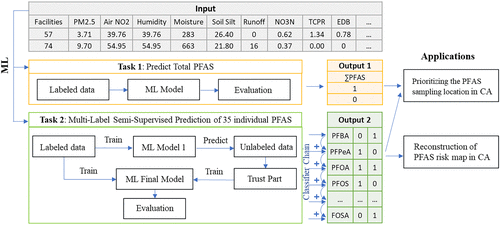
\includegraphics[width=0.95\linewidth]{Chap2/images/pipeline_dong.png}
    \caption{Pipeline bi-t\^ache de Dong et al.~\cite{dong2024pfas}. La t\^ache~1 (criblage total) repose sur une for\^et al\'eatoire avec sur-\'echantillonnage ADASYN~; la t\^ache~2 (pr\'ediction des 35 analytes) encha\^ine un pseudo-\'etiquetage semi-supervis\'e et une cha\^ine de classifieurs XGBoost. Les 112 variables contextuelles constituent l'unique entr\'ee, sans aucune concentration PFAS mesur\'ee.}
    \label{fig:dong-pipeline}
\end{figure}

Les deux t\^aches partagent le m\^eme vecteur de variables contextuelles~: la t\^ache~2 l'enrichit des seules \'etiquettes pr\'edites par la cha\^ine, jamais de concentrations mesur\'ees, ce qui maintient l'ensemble du dispositif dans le r\'egime pr\'edictif (section~\ref{sec:chap2-modes}).

% =========================================================
\mySection{Discussion}{}
\label{sec:chap2-discussion}
% =========================================================

\mySubSection{Tableau comparatif synth\'etique}{}
\label{sec:chap2-tableau}

Le tableau~\ref{tab:chap2-comparatif} synth\'etise les travaux examin\'es selon leur mode d'\'evaluation dominant, leur t\^ache et leurs m\'etriques.

\begin{table}[h!]
    \centering
    \caption{Synth\`ese comparative des approches de pr\'ediction PFAS examin\'ees. Les m\'etriques proviennent des articles sources~; protocoles et corpus diff\`erent entre \'etudes. $^*$~: pr\'esence de concentrations PFAS ou de signatures chimiques mesur\'ees dans les features.}
    \label{tab:chap2-comparatif}
    \small
    \begin{tabular}{p{2.6cm}p{2.8cm}p{2.4cm}p{1.6cm}p{2.6cm}}
        \hline
        R\'ef\'erence & M\'ethode & M\'etrique & Mode & T\^ache \\
        \hline
        Li et al.~\cite{li2022pfas} & R\'eseaux bay\'esiens & ROC-AUC $\approx 0{,}78$--$0{,}96$ & Mixte & PFAS ch. courte (MN) \\
        Hu et al.~\cite{hu2021privatewells} & Stats. contextuelles & (cartes) & Pr\'edictif pur & Vuln. puits priv\'es \\
        McMahon et al.~\cite{mcmahon2022pfas} & BRT & (descriptif) & Descriptif & Profils r\'egionaux \\
        George \& Dixit~\cite{george2021pfas} & RF / XGBoost & F1 $\approx 0{,}96/0{,}88^*$ & Mixte$^*$ & Priorisation bin. (CA) \\
        Tokranov et al.~\cite{tokranov2024pfas} & XGBoost & (national) & Mixte$^*$ & Vuln. nationale US \\
        Kibbey et al.~\cite{kibbey2020pfas} & ML supervis\'e & Pr\'ec. $\approx 90\,\%^*$ & Diagnostique & Attribution sources \\
        D\'avila-Santiago et al.~\cite{davilasantiago2022} & ML non cibl\'e & (relatif) & Diagnostique & NTS fingerprinting \\
        Cheng et Ng~\cite{cheng2019pfas} & QSAR/DNN & ROC-AUC moy. 0{,}916 & Mol\'eculaire & Bioactivit\'e mol. \\
        Dong et al.~\cite{dong2024pfas} & Semi-sup., CC & ROC-AUC 0{,}94--0{,}99 (T1) ; 0{,}73--1{,}00 (T2) & Pr\'edictif (ctx) & 35 analytes (CA) \\
        \hline
    \end{tabular}
\end{table}

On observe que les publications affichant les meilleurs scores (F1~$> 0{,}90$) mobilisent presque syst\'ematiquement des donn\'ees analytiques PFAS dans leurs entr\'ees.
Deux travaux seulement (Hu et al.\ et Dong et al.) \'evaluent leur mod\`ele en mode pr\'edictif strict~; cette lacune de documentation n'est pas anodine~: un praticien qui lit F1~$= 0{,}96$ dans un article peut croire disposer d'un outil op\'erationnel de priorisation avant analyse, alors qu'il s'agit en r\'ealit\'e d'un outil de compl\'etude d'un profil analytique partiellement connu.
Aucune \'etude publi\'ee ne compare les deux modes sur le m\^eme corpus avec le m\^eme protocole de division par site.


\mySubSection{Lecture transversale~: convergences et enseignements}{}
\label{sec:chap2-convergences}

Trois enseignements transversaux ressortent de la lecture crois\'ee des dix travaux.

\textbf{La proximit\'e industrielle est le signal le plus robuste.}
La proximit\'e aux bases militaires, aux usines fluorochimiques et aux a\'eroports ressort en t\^ete des variables explicatives dans des contextes g\'eologiques tr\`es diff\'erents, qu'elle soit mesur\'ee par les importances SHAP (George et Dixit, Tokranov, Dong et al.) ou par les ar\^etes du r\'eseau bay\'esien (Li et al.).
Ce r\'esultat constitue un fondement solide pour la s\'election des features contextuelles.

\textbf{La compl\'ementarit\'e tabulaire/relationnelle est structurellement fond\'ee.}
L'exploitation de la structure relationnelle entre analytes am\'eliore les scores par rapport aux mod\`eles tabulaires ind\'ependants~: les cha\^ines de classifieurs de Dong et al.\ en fournissent la seule d\'emonstration publi\'ee sur les PFAS.
La structure relationnelle entre puits voisins, attendue m\'ecanistiquement (section~\ref{sec:chap2-transport}), n'a en revanche pas encore \'et\'e \'evalu\'ee dans la litt\'erature PFAS~: les features contextuelles encodent le risque statique, tandis que la topologie d'\'ecoulement, encore inexploit\'ee, encoderait la corr\'elation spatiale entre puits voisins et la proximit\'e aux sources anthropiques.

\textbf{Le mode d'\'evaluation conditionne les performances de fa\c con fondamentale.}
Les \'etudes dont les features comprennent des concentrations PFAS mesur\'ees publient des scores bien sup\'erieurs (F1~$> 0{,}90$) \`a celles qui s'appuient exclusivement sur des variables contextuelles.
Cette diff\'erence ne refl\`ete pas un surcro\^it de qualit\'e algorithmique~: elle quantifie la valeur informative des mesures de laboratoire, et ne vaut que si l'on compare strictement le m\^eme mod\`ele dans les deux modes sur un m\^eme ensemble de test.


\mySubSection{Lacunes structurelles identifi\'ees}{}
\label{sec:chap2-lacunes}

L'examen crois\'e des travaux r\'ev\`ele quatre lacunes structurelles.

\paragraph{L1 -- Structure relationnelle sous-exploit\'ee.}
La majorit\'e des \'etudes tabulaires ignore les liens entre puits voisins, panaches et sources communes.
Les graphes h\'et\'erog\`enes~\cite{hu2020hgt} comblent partiellement ce vide, mais la sensibilit\'e des performances aux choix de construction du graphe (seuil de distance pour les ar\^etes, nombre de types de n\oe uds, dimension de l'embedding) n'a pas fait l'objet d'une \'etude de sensibilit\'e syst\'ematique dans la litt\'erature publi\'ee.
La question de la sensibilit\'e au seuil de distance et au nombre de types de n\oe uds reste ouverte.

\paragraph{L2 -- Biais d'\'evaluation circulaire.}
Plusieurs publications pr\'esentent des scores tr\`es \'elev\'es (F1~$> 0{,}90$) sans pr\'eciser si des concentrations PFAS mesur\'ees figurent dans les features~\cite{george2021pfas}.
Peu de travaux documentent simultan\'ement les deux modes sur le m\^eme corpus~; aucune \'etude publi\'ee ne compare les deux modes avec le m\^eme protocole de division strictement par site.
La v\'erification de l'absence de fuite d'information entre variables contextuelles et concentrations PFAS est une \'etape m\'ethodologique souvent omise.

\paragraph{L3 -- Transf\'erabilit\'e g\'eographique non valid\'ee.}
Les mod\`eles sont entra\^in\'es et test\'es sur une seule r\'egion (Californie, Minnesota, est des \'Etats-Unis).
Les validations crois\'ees spatiales (entra\^inement sur un aquif\`ere, test sur un autre de lithologie diff\'erente) restent pratiquement absentes.
Pour les graphes h\'et\'erog\`enes, la question est architecturalement profonde~: le graphe \'etant construit sur les n\oe uds d'entra\^inement, une approche inductive~\cite{hamilton2017inductive} (GraphSAGE) serait requise pour g\'en\'eraliser \`a des n\oe uds non vus.

\paragraph{L4 -- Interpr\'etabilit\'e insuffisamment standardis\'ee.}
Si SHAP~\cite{lundberg2017shap} s'impose progressivement comme standard, les protocoles varient fortement entre \'etudes.
Les pipelines hybrides graphe et boosting soul\`event des questions sp\'ecifiques non encore codifi\'ees~: comment interpr\'eter la contribution d'un embedding HGT agr\'egeant l'information de dizaines de n\oe uds voisins~? Comment comparer des valeurs TreeSHAP exactes (XGBoost, LightGBM) \`a des estimations SHAP Kernel approximatives (HGT)~? Une variable tabulaire fortement corr\'el\'ee \`a $\texttt{HGT\_emb\_0}$ verra sa valeur SHAP individuelle r\'eduite par interaction, rendant son importance marginale sous-estim\'ee.

\paragraph{Remarque sur le p\'erim\`etre g\'eographique de la revue.}
L'ensemble des travaux examin\'es porte sur des aquif\`eres nord-am\'ericains~; aucune \'etude comparable mobilisant l'apprentissage automatique sur des donn\'ees PFAS europ\'eennes ou africaines n'a \'et\'e identifi\'ee dans la litt\'erature publi\'ee.
Cette limitation intrins\`eque de la revue m\'erite d'\^etre signal\'ee~: les enseignements sur les variables pr\'edictives et les architectures restent transposables, mais les seuils r\'eglementaires (directive~UE~2020/2184~\cite{eu2020drinkingwater} vs EPA 2023~\cite{epa2023npdwr}), les contextes g\'eologiques et les pratiques de surveillance diff\`erent sensiblement.

Le tableau~\ref{tab:synthese-positionnement} positionne les principales contributions au regard de ces quatre lacunes.

\begin{table}[h!]
    \centering
    \caption{Positionnement des principales contributions au regard des quatre lacunes identifi\'ees. $\bullet$~: lacune adress\'ee~; $\circ$~: partiellement adress\'ee~; $\times$~: non adress\'ee. L1~: structure relationnelle~; L2~: biais confirmatoire~; L3~: transfert g\'eographique~; L4~: interpr\'etabilit\'e standardis\'ee.}
    \label{tab:synthese-positionnement}
    \small
    \begin{tabular}{lcccc}
        \hline
        R\'ef\'erence & L1 & L2 & L3 & L4 \\
        \hline
        Li et al.~\cite{li2022pfas}            & $\times$ & $\circ$ & $\times$ & $\times$ \\
        George et Dixit~\cite{george2021pfas}  & $\times$ & $\times$ & $\times$ & $\circ$ \\
        McMahon et al.~\cite{mcmahon2022pfas}  & $\times$ & $\circ$ & $\circ$  & $\times$ \\
        Tokranov et al.~\cite{tokranov2024pfas} & $\times$ & $\circ$ & $\bullet$ & $\circ$ \\
        Dong et al.~\cite{dong2024pfas}        & $\times$ & $\times$ & $\times$ & $\circ$ \\
        \hline
    \end{tabular}
\end{table}

Aucun travail de la litt\'erature n'adresse simultan\'ement L1, L2 et L4~: les \'etudes tabulaires ignorent la structure relationnelle~; celles qui exploitent un graphe ne documentent pas le mode pr\'edictif strict~; l'interpr\'etabilit\'e reste non standardis\'ee.
La combinaison de ces lacunes, en particulier la validation inter-aquif\`eres (L3), d\'efinit autant de directions de recherche encore ouvertes.


% =========================================================
\mySection{Synth\`ese}{}
\label{sec:synthese-chap2}
% =========================================================

Ce chapitre a dress\'e un panorama structur\'e de l'application de l'intelligence artificielle \`a la pr\'ediction et \`a la surveillance des PFAS en eaux souterraines.
La premi\`ere g\'en\'eration (mod\`eles probabilistes et arbres d'ensemble) a \'etabli le socle des variables pr\'edictives (proximit\'e aux sources, indicateurs hydrog\'eologiques, co-contaminants) et d\'emontr\'e la faisabilit\'e de la priorisation r\'egionale et nationale.
La deuxi\`eme (r\'eseaux de neurones, puis cha\^ines semi-supervis\'ees multi-\'etiquettes) a \'etendu le champ \`a plusieurs dizaines d'analytes et exploit\'e les donn\'ees non \'etiquet\'ees, sans toujours expliciter le r\'egime d'\'evaluation retenu.

Les lacunes L1--L4 dessinent en creux un syst\`eme id\'eal de priorisation~: fonctionnant sans mesure PFAS pr\'ealable (mode pr\'edictif pur), int\'egrant les relations spatiales par un graphe h\'et\'erog\`ene, interpr\'etable par SHAP globale et locale, et valid\'e sur une division spatiale ind\'ependante.
Aucune \'etude publi\'ee ne satisfait simultan\'ement ces crit\`eres.

	\myChapter{Contribution~: enrichissement g\'eospatial g\'en\'erique et pr\'ediction du risque PFAS}{Contribution~: enrichissement g\'eospatial g\'en\'erique et pr\'ediction du risque PFAS}
\label{chap:contribution}
\myMiniToc{section}{Sommaire}

% =========================================================
\mySection{Introduction}{}
\label{sec:contrib-intro}
% =========================================================

Le chapitre~\ref{chap:etat-art} a d\'egag\'e quatre lacunes structurelles dans la litt\'erature de pr\'ediction des PFAS par apprentissage automatique (section~\ref{sec:chap2-lacunes})~: la structure relationnelle entre forages voisins, panaches et sources communes reste sous-exploit\'ee (L1)~; un biais d'\'evaluation circulaire appara\^it lorsque des concentrations PFAS mesur\'ees se glissent dans les variables, sans s\'eparer clairement le mode pr\'edictif du mode confirmatoire (L2)~; la transf\'erabilit\'e g\'eographique est rarement valid\'ee, faute de validation crois\'ee spatiale inter-aquif\`eres (L3)~; et l'interpr\'etabilit\'e demeure peu standardis\'ee, en particulier pour les pipelines hybrides combinant graphe et boosting (L4). Aucune \'etude publi\'ee ne traite simultan\'ement de ces quatre lacunes. Ce chapitre pr\'esente une contribution qui y r\'epond directement, sur le cas de la contamination des eaux souterraines californiennes.

Le support empirique est un jeu de donn\'ees r\'ecent rassemblant des dizaines de milliers de mesures de PFAS sur l'ensemble de la Californie~\cite{dong2024pfas}, dont la cible est le d\'epassement des limites r\'eglementaires fix\'ees en 2024 (section~\ref{sec:pfas-reglementation})~\cite{epa2023npdwr}. La contamination n'y est pas explicable par la seule mesure ponctuelle d'un forage~: elle d\'epend du contexte (proximit\'e de sources industrielles ou militaires, nature du sol, hydrog\'eologie, co-polluants). Exploiter ce contexte, et la structure relationnelle vis\'ee par la lacune L1, suppose d'abord d'attacher \`a chaque observation des variables environnementales g\'eor\'ef\'erenc\'ees, op\'eration aujourd'hui assur\'ee par des scripts li\'es \`a un jeu de donn\'ees particulier et difficilement r\'eutilisables.

La contribution comporte deux volets. Le premier est un outil, \texttt{geoenrich}, moteur d'enrichissement g\'eospatial g\'en\'erique fond\'e sur un contrat d'entr\'ee minimal et une biblioth\`eque d'op\'erateurs enfichables, ind\'ependant du jeu PFAS qui lui a servi de banc d'essai~: il fournit le socle de variables de contexte et la base reproductible sur lesquels reposent les mod\`eles. Le second est un banc de cinq mod\`eles compar\'es \`a protocole identique (deux mod\`eles tabulaires de r\'ef\'erence, un transformeur de graphe h\'et\'erog\`ene et deux mod\`eles hybrides), con\c{c}u pour r\'epondre aux lacunes L1, L2 et L4. Tous op\`erent en \textbf{mode pr\'edictif} strict (section~\ref{sec:chap2-modes})~: aucune concentration PFAS n'entre dans leurs variables, ce qui \'ecarte le biais confirmatoire (L2). La localisation est retir\'ee des variables de tous les mod\`eles et ne subsiste que dans la topologie d'un graphe relationnel (L1), afin de tester si le signal spatial doit \^etre m\'emoris\'e comme variable ou structur\'e dans le graphe. L'interpr\'etabilit\'e globale et locale accompagne chaque mod\`ele (L4), tandis que la transf\'erabilit\'e g\'eographique (L3) est pos\'ee comme perspective ouverte, la validation crois\'ee spatiale par blocs n'ayant pas \'et\'e ex\'ecut\'ee dans ce travail. La suite est organis\'ee comme suit~: la section~\ref{sec:contrib-vue} pr\'esente la vue d'ensemble~; la section~\ref{sec:geoenrich} d\'ecrit \texttt{geoenrich}~; la section~\ref{sec:contrib-modeles} expose les mod\`eles~; la section~\ref{sec:contrib-resultats} rassemble les r\'esultats, leur interpr\'etabilit\'e et leur discussion~; la section~\ref{sec:synthese-chap3} conclut.


% =========================================================
\mySection{Vue d'ensemble de l'approche}{}
\label{sec:contrib-vue}
% =========================================================

Avant d'entrer dans le d\'etail de l'outil puis des mod\`eles, cette section d\'ecrit la cha\^ine de traitement dans son ensemble et les principes qui en gouvernent la conception, de l'observation brute jusqu'\`a la pr\'ediction interpr\'et\'ee.

\mySubSection{Pipeline de traitement de bout en bout}{}
\label{sec:contrib-chaine}

Le pipeline s'articule en quatre \'etapes. En entr\'ee, des observations ponctuelles~: pour chaque pr\'el\`evement, un identifiant, une position g\'eographique et une date. Ces observations passent d'abord par l'\'etape d'enrichissement, qui leur attache des dizaines de variables contextuelles (sols, hydrologie, sources de contamination, co-polluants, unit\'es hydrog\'eologiques). Le jeu enrichi alimente ensuite le pr\'etraitement (d\'efinition de la cible r\'eglementaire, s\'election et nettoyage des variables, d\'ecoupage), puis la mod\'elisation qui entra\^ine et compare plusieurs pr\'edicteurs. La derni\`ere \'etape, \'evaluation et interpr\'etation, mesure les performances, rend les d\'ecisions lisibles et restitue les pr\'edictions sous forme cartographique. La figure~\ref{fig:schema1} en donne la vue d'ensemble.

\begin{figure}[H]
    \centering
    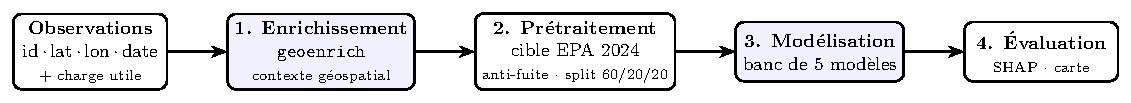
\includegraphics[width=0.92\linewidth]{Chap3/images/latex/schema1.pdf}
    \caption{Vue d'ensemble du pipeline, de l'observation ponctuelle \`a l'\'evaluation interpr\'et\'ee.}
    \label{fig:schema1}
\end{figure}

Cette lin\'earit\'e apparente masque une distinction structurante, introduite d\`es la premi\`ere \'etape et reprise dans tout le travail~: la s\'eparation entre la \emph{charge utile} (ce que l'on mesure et cherche \`a pr\'edire) et le \emph{contexte g\'eographique} (o\`u et quand la mesure a \'et\'e faite). La figure~\ref{fig:schema1bis} d\'etaille l'architecture interne de chaque \'etape.

\begin{figure}[H]
    \centering
    
\includegraphics[width=0.92\linewidth]{Chap3/images/mermaid/schema1bis.png}
    \caption{Architecture interne des \'etapes~: enrichissement (\texttt{geoenrich}), pr\'etraitement (cible EPA 2024, anti-fuite, d\'ecoupage) et mod\'elisation (banc de cinq mod\`eles).}
    \label{fig:schema1bis}
\end{figure}

\mySubSection{Du jeu d'observations au dataset enrichi}{}
\label{sec:contrib-enrichissement-principe}

L'enrichissement repose sur une id\'ee directrice~: tout le contexte g\'eographique d'une observation se d\'eduit de son \emph{o\`u} et de son \emph{quand}, ind\'ependamment de la nature de ce qui est mesur\'e. Un op\'erateur qui calcule la distance au site de contamination le plus proche, ou qui rattache un point \`a son sous-bassin hydrog\'eologique, n'a pas besoin de savoir s'il manipule une mesure de PFAS, de nitrate ou de m\'etaux~: il n'utilise que les coordonn\'ees et la date. La charge utile est transport\'ee sans jamais \^etre lue.

Cette s\'eparation r\'eduit le contrat d'entr\'ee \`a quatre champs canoniques (identifiant, latitude, longitude, date), auxquels n'importe quel jeu d'observations peut \^etre ramen\'e, le reste des colonnes \'etant consid\'er\'e comme charge utile ignor\'ee. L'enrichissement devient alors une op\'eration g\'en\'erique, applicable au-del\`a du cas PFAS qui lui a servi d'instanciation. Sur le dataset californien, cette \'etape attache aux mesures un large \'eventail de variables de contexte (proximit\'e et densit\'e de sites de contamination, propri\'et\'es des sols, variables hydrog\'eologiques, sous-bassins), dont la validit\'e a \'et\'e contr\^ol\'ee par comparaison avec le pipeline initial du projet.

\mySubSection{De l'enrichissement \`a la pr\'ediction}{}
\label{sec:contrib-enrichissement-prediction}
Le dataset enrichi sert de socle commun \`a tous les mod\`eles, ce qui garantit une comparaison \'equitable. Sur ce socle, deux familles de mod\`eles cohabitent. Les mod\`eles tabulaires (for\^et al\'eatoire, gradient boosting) traitent chaque observation comme un vecteur de variables ind\'ependant des autres. Le mod\`ele relationnel (transformeur de graphe h\'et\'erog\`ene) exploite au contraire la structure~: il relie les forages entre eux et \`a des entit\'es partag\'ees (sites de contamination, sous-bassins, voisinages spatiaux) de sorte que des points proches d'une m\^eme source \'echangent de l'information.
Deux mod\`eles hybrides compl\`etent le banc, en combinant les repr\'esentations apprises par le graphe avec les variables tabulaires.

\mySubSection{Principes directeurs}{}
\label{sec:contrib-principes}

Trois principes traversent l'ensemble de la contribution. Le premier est la r\'eutilisabilit\'e de l'outil~: l'enrichissement est con\c{c}u comme un composant g\'en\'erique, le moteur ne contenant aucune r\'ef\'erence au cas PFAS, les sp\'ecificit\'es r\'egionales \'etant rel\'egu\'ees dans une configuration externe rempla\c{c}able sans toucher au code. Le deuxi\`eme est la rigueur de l'\'evaluation~: le dispositif central contre la m\'emorisation g\'eographique est le retrait de la localisation des variables d'entr\'ee, combin\'e \`a sa structuration dans la topologie du graphe relationnel. Le troisi\`eme est l'interpr\'etabilit\'e comme exigence transversale~: chaque mod\`ele est accompagn\'e d'analyses d'importance des variables et d'explications locales, la lisibilit\'e \'etant trait\'ee comme un livrable \`a part enti\`ere dans un contexte environnemental o\`u les pr\'edictions orientent des d\'ecisions de surveillance.


% =========================================================
\mySection{\texttt{geoenrich}~: un moteur d'enrichissement g\'eospatial g\'en\'erique}{}
\label{sec:geoenrich}
% =========================================================

La premi\`ere contribution est un outil~: \texttt{geoenrich}\footnote{D\'ep\^ot public~: \url{https://github.com/dnwiloic/geoenrich}}. Il produit, \`a partir d'un jeu d'observations ponctuelles respectant un contrat d'entr\'ee minimal, un dataset riche en variables contextuelles via une biblioth\`eque d'op\'erateurs enfichables. Le dataset PFAS californien en est la premi\`ere instanciation et non une d\'ependance.

\mySubSection{Motivation}{}
\label{sec:geoenrich-motivation}


La plupart des jeux de donn\'ees consacr\'es aux PFAS pr\'esentent un nombre limit\'e de caract\'eristiques. Ils se limitent g\'en\'eralement aux informations relatives aux puits (localisation, cote ou profondeur), \`a la date de pr\'el\`evement ainsi qu'aux r\'esultats des analyses de laboratoire. Or, la litt\'erature a montr\'e que les informations contextuelles, telles que la proximit\'e et la densit\'e des sites potentiels de contamination, les propri\'et\'es des sols, les variables hydrog\'eologiques ou encore les sous-bassins versants, jouent un r\^ole essentiel dans la pr\'ediction des risques li\'es aux PFAS \`a l'aide de m\'ethodes d'intelligence artificielle~\cite{dong2024pfas,guelfo2021pfas}. L'objectif de \texttt{geoenrich} est donc d'enrichir automatiquement ces jeux de donn\'ees en leur ajoutant des caract\'eristiques environnementales pertinentes, d\'eriv\'ees de la localisation des puits et de la date de pr\'el\`evement, afin d'am\'eliorer les performances des mod\`eles de pr\'ediction.
% Le code initial du projet illustrait le travers des scripts ad hoc~: la logique de jointure tenait dans un module unique de pr\`es de mille lignes, o\`u la m\'ecanique g\'en\'erique d'appariement spatial et temporel se trouvait m\^el\'ee aux particularit\'es du cas PFAS (noms de colonnes propres au programme de surveillance, chemins de couches sp\'ecifiques, r\`egles m\'etier li\'ees au polluant). Un tel code n'est ni testable isol\'ement, ni r\'eutilisable~: changer de polluant ou de r\'egion imposerait de le r\'e\'ecrire. L'objectif de \texttt{geoenrich} est de transformer cette logique monolithique en un composant r\'eutilisable, par une s\'eparation stricte entre le \emph{quoi} (la mesure \'etudi\'ee, simple charge utile transport\'ee) et le \emph{o\`u/quand} (les cl\'es de jointure universelles que sont la position et la date).

\mySubSection{Contrat d'entr\'ee}{}
\label{sec:geoenrich-contrat}

Le contrat d'entr\'ee est l'interface minimale que tout jeu d'observations doit satisfaire pour \^etre enrichi. Il se r\'eduit \`a quatre champs canoniques~: un identifiant de point, une latitude et une longitude en WGS84 (cl\'es de jointure spatiale), et une date (cl\'e de jointure temporelle). Seules la latitude et la longitude sont strictement obligatoires~; l'identifiant est g\'en\'er\'e \`a d\'efaut, et la date n'est requise que si des op\'erateurs temporels sont mobilis\'es. Toute autre colonne est consid\'er\'ee comme charge utile et n'est jamais lue par le moteur. Une fonction de mise au contrat renomme les colonnes du jeu source vers ces noms canoniques, puis une \'etape de validation contr\^ole le typage, supprime les lignes sans coordonn\'ees et analyse les dates. C'est cette r\'eduction \`a quatre champs qui rend le moteur agnostique.

\mySubSection{Architecture en trois couches}{}
\label{sec:geoenrich-architecture}

L'architecture de \texttt{geoenrich} repose sur trois couches strictement s\'epar\'ees, dont la g\'en\'ericit\'e d\'ecro\^it \`a mesure que l'on descend vers le cas concret (figure~\ref{fig:schema2}). La \textbf{couche contrat}, sup\'erieure, est enti\`erement agnostique~: elle ne conna\^it que les quatre cl\'es canoniques et ignore la charge utile. La \textbf{couche op\'erateurs}, interm\'ediaire, rassemble les op\'erateurs d'enrichissement, g\'en\'eriques mais param\'etrables, qui reposent sur deux primitives de jointure seulement~: une primitive spatiale fond\'ee sur un arbre k-d en distance grand-cercle (point source le plus proche, sources dans un rayon, polygone contenant un point) et une primitive temporelle par appariement par ant\'eriorit\'e par entit\'e, avec repli spatial lorsque l'appariement direct \'echoue. La couche configuration, inf\'erieure, est la seule \`a porter le contexte particulier d'une r\'egion~: un fichier YAML d\'eclare la racine des donn\'ees de r\'ef\'erence et la liste ordonn\'ee des op\'erateurs, chacun pointant vers ses couches locales. Un registre interne associe chaque type d'op\'erateur \`a sa classe d'impl\'ementation, de sorte qu'ajouter un op\'erateur ne demande qu'une ligne de configuration, sans modifier le code.

\begin{figure}[H]
    \centering
    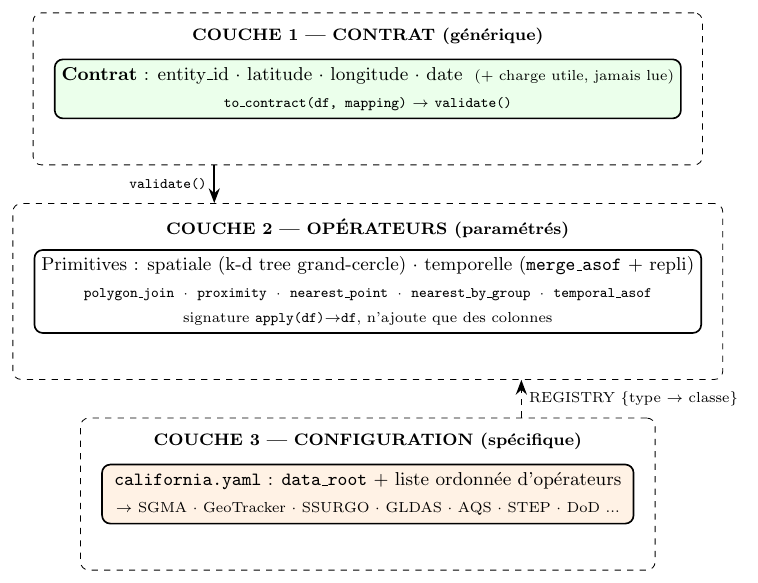
\includegraphics[width=0.88\linewidth]{Chap3/images/latex/schema2.png}
    \caption{Les trois couches de \texttt{geoenrich}~: contrat agnostique, op\'erateurs param\'etr\'es (primitives spatiale et temporelle), configuration sp\'ecifique \`a la r\'egion.}
    \label{fig:schema2}
\end{figure}

\mySubSection{Biblioth\`eque d'op\'erateurs}{}
\label{sec:geoenrich-operateurs}

La biblioth\`eque compte cinq familles d'op\'erateurs, chacune r\'epondant \`a un motif de jointure r\'ecurrent~: \texttt{polygon\_join} rattache un point aux attributs du polygone qui le contient (par exemple le sous-bassin hydrog\'eologique d'un forage)~; \texttt{proximity} calcule la distance au site le plus proche, son type et le nombre de sites dans une s\'erie de rayons~; \texttt{nearest\_point} r\'ecup\`ere les valeurs du point source le plus proche, en version statique ou index\'ee par ann\'ee et par mois~; \texttt{nearest\_by\_group} traite les sources au format long en retrouvant, pour chaque code de variable, le moniteur le plus proche~; \texttt{temporal\_asof} r\'ealise l'appariement temporel par entit\'e avec repli spatial. Ces op\'erateurs partagent quatre propri\'et\'es qui font la robustesse du moteur~: ils sont composables, optionnels (un op\'erateur dont la source est absente est ignor\'e sans interrompre le traitement), idempotents sur le contrat (ils n'ajoutent que des colonnes) et ind\'ependants de la charge utile.

\mySubSection{Entr\'ees, sorties et instanciation californienne}{}
\label{sec:geoenrich-io}

En entr\'ee, \texttt{geoenrich} accepte des observations ponctuelles aux formats CSV, Parquet ou GeoJSON, ramen\'ees au contrat par leur mapping. La sortie est le m\^eme jeu, augment\'e des colonnes produites par chaque op\'erateur et accompagn\'e d'un dictionnaire de donn\'ees d\'ecrivant les variables g\'en\'er\'ees. L'outil s'utilise comme biblioth\`eque Python et en ligne de commande. Pour le cas californien, la configuration instancie neuf op\'erateurs mobilisant autant de couches de r\'ef\'erence~: sous-bassins hydrog\'eologiques, sites de contamination, stations d'\'epuration, sites f\'ed\'eraux li\'es \`a la d\'efense (source majeure de PFAS par les mousses anti-incendie, section~\ref{sec:pfas-usages-sources}), d\'echarges, propri\'et\'es des sols, variables hydrologiques mensuelles, qualit\'e de l'air et co-contaminants par appariement temporel, auxquels s'ajoutent l'occupation du sol et la topographie extraites par \'echantillonnage raster. \`A partir des seules coordonn\'ees et dates, l'ensemble produit un contexte environnemental riche pour chaque mesure.

\mySubSection{Le jeu de donn\'ees d'application~: de la base GAMA au dataset enrichi}{}
\label{sec:geoenrich-dataset}

L'instanciation californienne de \texttt{geoenrich} produit le jeu de donn\'ees qui sert \`a entra\^iner et \'evaluer les mod\`eles de la section~\ref{sec:contrib-modeles}. Cette sous-section en d\'ecrit l'origine, la base d'observations brutes, puis le jeu enrichi et son remplissage.

\mySubSubSection{Origine et reconstruction de la base}{}
\label{sec:geoenrich-dataset-origine}

Le dataset qui sert de base pour l'enrichissement a \'et\'e constitu\'e \`a partir de deux fichiers bruts du programme GAMA, \texttt{gama\_allwells}\footnote{\url{https://data.ca.gov/dataset/ground-water-water-quality-results/resource/805e6762-1b82-48d9-b68f-5d79cca06ace}} et \texttt{pfas}\footnote{\url{https://data.ca.gov/dataset/ground-water-water-quality-results/resource/c7cd50a2-2a68-44a1-8d40-4e767f363964}}. La fusion consiste \`a ramener toutes les mesures de contaminant d'un puits ainsi que la date de pr\'el\`evement sur une m\^eme ligne contenant \'egalement les coordonn\'ees g\'eographiques du puits. Cette op\'eration a pour but de respecter le contrat d'entr\'ee de \texttt{geoenrich}. Le dataset obtenu, nomm\'e \texttt{wells\_pfas\_cleaned}, couvre 46\,338 pr\'el\`evements sur environ 11\,300 puits, r\'epartis sur les 58 comt\'es de l'\'Etat, entre avril 2016 et janvier 2026, un p\'erim\`etre plus large et plus r\'ecent que celui de Dong et al.~\cite{dong2024pfas}. Chaque pr\'el\`evement porte une cl\'e d'identit\'e minimale et ses mesures comme indiqu\'e dans le tableau~\ref{tab:base-brute}.

\begin{table}[h!]
    \centering
    \caption{Familles de colonnes de la base d'observations brutes (avant enrichissement).}
    \label{tab:base-brute}
    \small
    \begin{tabular}{l p{5.3cm} p{4.6cm}}
        \hline
        Cat\'egorie & Colonnes (exemples) & R\^ole \\
        \hline
        Identit\'e & \texttt{gm\_well\_id}, \texttt{gm\_dataset\_name}, \texttt{gm\_well\_category} & puits, programme source (6), type de puits (5) \\
        Localisation & \texttt{latitude}, \texttt{longitude}, \texttt{county}, \texttt{regional\_board} & cl\'es spatiales, d\'ecoupage administratif \\
        Temps & \texttt{collection\_date} & date du pr\'el\`evement (2\,069 dates distinctes) \\
        Mesures PFAS & 32 colonnes \texttt{*\_ngL} & concentrations par esp\`ece (PFOA, PFOS, PFHxS, PFBS, etc.) \\
        D\'etection & 62 colonnes \texttt{*\_detected}, \texttt{label\_*} & indicateurs de d\'etection par esp\`ece \\
        \hline
    \end{tabular}
\end{table}

La caract\'eristique notable de cette base est que les concentrations elles-m\^emes sont tr\`es lacunaires~: toutes les esp\`eces ne sont pas dos\'ees \`a chaque pr\'el\`evement, si bien que la majorit\'e des 32 colonnes \texttt{*\_ngL} d\'epasse 40~\% de valeurs manquantes. Ces colonnes d\'efinissent la cible et sont \'ecart\'ees comme fuite (section~\ref{sec:contrib-pretraitement})~; leur lacune n'affecte donc pas la mod\'elisation. Hors PFAS, la base brute n'apporte qu'un contexte tr\`es limit\'e, d'o\`u le recours \`a l'enrichissement.

\mySubSubSection{Le jeu enrichi~: structure et familles de colonnes}{}
\label{sec:geoenrich-dataset-enrichi}

Apr\`es passage par \texttt{geoenrich}, le jeu compte 217 colonnes (131 r\'eelles, 41 enti\`eres, 31 bool\'eennes, 13 textuelles, 1 date) pour les m\^emes 46\,338 pr\'el\`evements. \`A la base s'ajoutent les familles de variables contextuelles r\'esum\'ees au tableau~\ref{tab:familles-enrichies}.

\begin{table}[h!]
    \centering
    \caption{Familles de variables contextuelles ajout\'ees par \texttt{geoenrich} (nombre de colonnes et taux moyen de valeurs manquantes).}
    \label{tab:familles-enrichies}
    \small
    \begin{tabular}{p{4.2cm} p{6.2cm} c c}
        \hline
        Famille (source) & Pr\'efixe / colonnes & Nb & NA \% moyen \\
        \hline
        Sites de contamination GeoTracker & \texttt{dist\_geotracker\_km}, \texttt{n\_geotracker\_within\_\{1,3,10,50\}km}, \texttt{nearest\_geotracker\_type} & 6 & 0 \\
        Co-contaminants (GAMA) & \texttt{cocontam\_*} & 44 & 16,5 \\
        Sol (SSURGO) & \texttt{soil\_*} & 26 & 20,5 \\
        Qualit\'e de l'air (AQS) & \texttt{aqs\_*} & 8 & 9,9 \\
        Hydrom\'et\'eorologie (GLDAS) & \texttt{rainfall\_mm\_month}, \texttt{et\_mm\_month}, \texttt{runoff\_mm}, \texttt{temp\_c}, \texttt{snowpack\_mm}, \texttt{root\_zone\_moist\_kg\_m2} & 7 & $\sim$4 \\
        Bassins hydrog\'eologiques (SGMA) & \texttt{sgma\_*} & 3 & 6,1 \\
        Niveaux de nappe et gradient (DWR) & \texttt{depth\_to\_water\_m}, \texttt{dist\_nearest\_gwl\_km}, \texttt{hydr\_grad\_mag\_permil}, \texttt{flow\_dir\_sin/cos} & 6 & $\sim$0 \\
        Topographie (USGS 3DEP) & \texttt{elevation\_m} & 1 & 10,4 \\
        Occupation du sol (NLCD) & \texttt{dev\_intensity}, \texttt{lc\_developed} & 2 & 0 \\
        G\'eom\'etrie de forage & \texttt{well\_depth\_ft}, \texttt{screen\_mid\_ft}, \texttt{screen\_length\_ft}, \texttt{depth\_eff\_ft} & 4 & 49 \`a 95 \\
        Indicateurs d'absence (ing\'enierie) & \texttt{depth\_missing}, \texttt{topo\_missing} & 2 & 0 \\
        \hline
    \end{tabular}
\end{table}

Ces familles couvrent les hypoth\`eses m\'ecanistes de la contamination~: proximit\'e des sources, nature du sol, hydrologie, co-pollution, contexte hydrog\'eologique.

\mySubSubSection{Remplissage des colonnes}{}
\label{sec:geoenrich-dataset-remplissage}

Le profil de compl\'etude du jeu enrichi est globalement favorable~: sur les 217 colonnes, 88 sont renseign\'ees \`a 100~\% et 80 le sont \`a plus de 90~\%. Les variables de contexte ajout\'ees par l'enrichissement spatial (proximit\'e GeoTracker, occupation du sol, niveaux de nappe) sont presque toujours compl\`etes, parce qu'elles r\'esultent d'une jointure g\'eographique qui aboutit pour tout point situ\'e dans l'emprise des couches de r\'ef\'erence.

Trente et une colonnes d\'epassent 40~\% de valeurs manquantes. Leur examen est rassurant~: 17 sont des concentrations \texttt{*\_ngL}, d\'ej\`a \'elimin\'ees comme fuite, et les 14 restantes se r\'epartissent entre la g\'eom\'etrie de forage (\texttt{well\_depth\_ft} \`a 95~\%, \texttt{screen\_*} et \texttt{depth\_eff\_*} autour de 50~\%, rarement document\'es dans GAMA), la granulom\'etrie fine du sol et quelques co-contaminants rares. Le signal hydrog\'eologique que portait la g\'eom\'etrie de forage est partiellement r\'ecup\'er\'e par des proxys mieux renseign\'es et conserv\'es, la profondeur de la nappe (\texttt{depth\_to\_water\_m}), la distance au point de mesure pi\'ezom\'etrique (\texttt{dist\_nearest\_gwl\_km}) et le gradient hydraulique (\texttt{hydr\_grad\_mag\_permil}), tous complets. Enfin, des indicateurs binaires d'absence (\texttt{depth\_missing}, \texttt{topo\_missing}) encodent explicitement la lacune sans inventer de valeur. C'est ce jeu enrichi, une fois \'ecart\'ees les colonnes de fuite, les variables trop lacunaires et la localisation, qui alimente les mod\`eles de la section~\ref{sec:contrib-modeles}.


% =========================================================
\mySection{Mod\`eles de pr\'ediction de la contamination}{}
\label{sec:contrib-modeles}
% =========================================================

La seconde contribution est un banc de cinq mod\`eles pr\'edisant, pour chaque pr\'el\`evement, le risque de d\'epassement du seuil r\'eglementaire EPA 2024. Tous partagent le m\^eme dataset enrichi, la m\^eme cible et le m\^eme d\'ecoupage, ce qui rend leur comparaison \'equitable (figure~\ref{fig:schema3}). Le fil directeur est la question de recherche pos\'ee en introduction (section~\ref{sec:contrib-intro})~: le signal spatial doit-il \^etre m\'emoris\'e comme variable ou structur\'e dans la topologie d'un graphe~? La r\'eponse op\'erationnelle est le retrait de la localisation de toutes les variables, celle-ci n'intervenant que dans la construction du graphe.

\begin{figure}[H]
    \centering
    
\includegraphics[width=0.92\linewidth]{Chap3/images/mermaid/schema3.png}
    \caption{Le banc des cinq mod\`eles sur socle commun (dataset enrichi, d\'ecoupage 60/20/20) et les d\'ependances des mod\`eles hybrides (fusion par embeddings, stacking).}
    \label{fig:schema3}
\end{figure}

On observe que les cinq mod\`eles partent du m\^eme dataset enrichi et du m\^eme d\'ecoupage 60/20/20, ce qui garantit une comparaison \'equitable~: les \'ecarts de performance mesur\'es plus loin tiennent au mod\`ele et non aux donn\'ees. La figure distingue aussi deux niveaux. Les deux arbres de r\'ef\'erence et le HGT s'entra\^inent directement sur le socle commun, tandis que les deux mod\`eles hybrides en d\'ependent~: la fusion par embeddings r\'eutilise les repr\'esentations apprises par le HGT, et le stacking combine les pr\'edictions des trois mod\`eles de base. Ces fl\`eches de d\'ependance expliquent l'ordre dans lequel les mod\`eles sont pr\'esent\'es et entra\^in\'es par la suite.

\mySubSection{Donn\'ees et cible}{}
\label{sec:contrib-donnees}

L'\'etude porte sur 46\,338 pr\'el\`evements d'eaux souterraines californiennes~\cite{dong2024pfas}, enrichis par \texttt{geoenrich} (section~\ref{sec:geoenrich}) puis ramen\'es \`a 97 variables explicatives apr\`es nettoyage (94 num\'eriques et 3 cat\'egorielles). Ces variables d\'ecrivent le contexte du forage (proximit\'e et densit\'e de sites de contamination, sol, hydrologie, qualit\'e de l'air, co-contaminants), \`a l'exclusion de toute concentration en PFAS, conform\'ement au mode pr\'edictif.

\paragraph{Construction de la cible}{}
\label{sec:contrib-cible}

La cible est binaire et reproduit la r\`egle de d\'epassement du r\`eglement EPA 2024 NPDWR (section~\ref{sec:pfas-reglementation})~\cite{epa2023npdwr}. Deux crit\`eres ind\'ependants peuvent la d\'eclencher, correspondant aux deux volets du r\`eglement.

Le \textbf{crit\`ere individuel} vaut 1 d\`es qu'une concentration mesur\'ee d\'epasse son MCL, fix\'e \`a 4~ng/L pour le PFOA et le PFOS, et \`a 10~ng/L pour le PFNA, le PFHxS et le HFPO-DA. Le \textbf{crit\`ere de m\'elange} s'appuie sur l'indice de risque (HI)~: il est d\'eclench\'e lorsque $\mathrm{HI} > 1$, c'est-\`a-dire lorsque les effets cumul\'es des compos\'es d\'epassent le niveau jug\'e admissible. Le tableau~\ref{tab:epa2024-seuils} r\'esume les six compos\'es couverts et les valeurs num\'eriques utilis\'ees.

\begin{table}[H]
    \centering
    \caption{Seuils EPA 2024 NPDWR impl\'ement\'es dans la construction de la cible.}
    \label{tab:epa2024-seuils}
    \begin{tabular}{lllcc}
        \hline
        Compos\'e & Sigle & Classe & MCL (ng/L) & $\mathrm{VR}_i$ HI (ng/L) \\
        \hline
        Acide perfluoroocta\-no\"ique       & PFOA    & PFCA & 4   & N.A.  \\
        Sulfonate de perfluorooctane        & PFOS    & PFSA & 4   & N.A.  \\
        Acide perfluorononano\"ique         & PFNA    & PFCA & 10  & 10   \\
        Acide perfluorohexane sulfonique    & PFHxS   & PFSA & 10  & 10   \\
        Acide dim\'erique HFPO (GenX)       & HFPO-DA & N.A. & 10  & 10   \\
        Acide perfluorobutane sulfonique    & PFBS    & PFSA & N.A. & 2000 \\
        \hline
    \end{tabular}
\end{table}

Le HI est calcul\'e sur les quatre compos\'es pour lesquels l'EPA fournit une valeur sanitaire de r\'ef\'erence $\mathrm{VR}_i$~:
\[
    \mathrm{HI}
    = \frac{C_{\mathrm{PFNA}}}{10}
    + \frac{C_{\mathrm{PFHxS}}}{10}
    + \frac{C_{\mathrm{HFPO\text{-}DA}}}{10}
    + \frac{C_{\mathrm{PFBS}}}{2000}
\]
o\`u toutes les concentrations $C_i$ sont exprim\'ees en ng/L. On notera que le PFNA, le PFHxS et le HFPO-DA figurent dans les deux crit\`eres~: d\'epasser 10~ng/L pour l'un de ces compos\'es d\'eclenche simultan\'ement le MCL individuel et alourdit le HI.

Un pr\'el\`evement est \'etiquet\'e \`a risque (cible $= 1$) d\`es qu'au moins l'un des deux crit\`eres est franchi, et conforme (cible $= 0$) sinon. Le calcul part des concentrations brutes~; les valeurs manquantes sont assimil\'ees \`a des non-d\'etections et contribuent donc pour z\'ero aux deux crit\`eres.

Le jeu obtenu est presque \'equilibr\'e~: 21\,154 pr\'el\`evements positifs (45,65~\% de l'\'echantillon), ce qui \'evite de recourir \`a un r\'e\'echantillonnage artificiel. La figure~\ref{fig:class-distribution} pr\'esente cette distribution.

\begin{figure}[H]
    \centering
    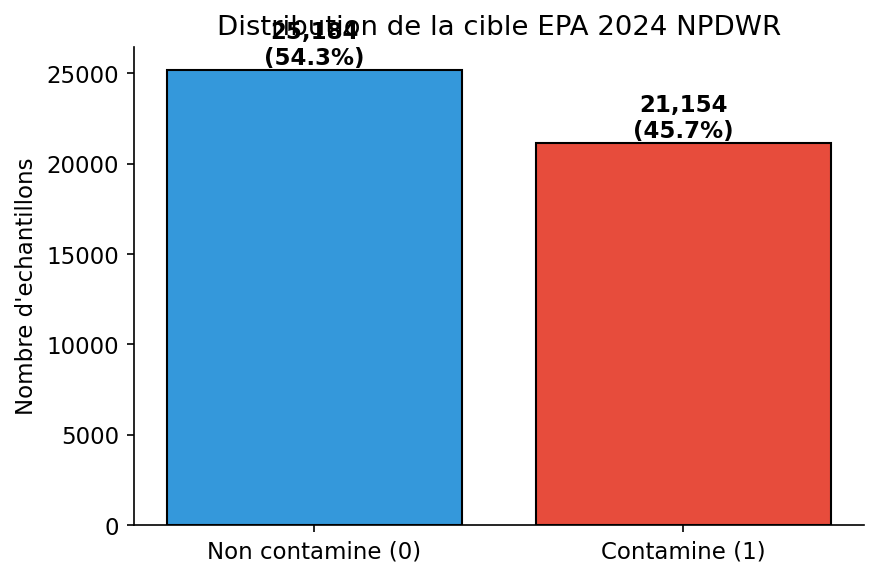
\includegraphics[width=0.6\linewidth]{Chap3/images/figures/fig01_class_distribution.png}
    \caption{Distribution des classes de la cible EPA 2024 sur le jeu complet.}
    \label{fig:class-distribution}
\end{figure}
On constate que les deux classes sont presque \'equilibr\'ees, ce qui justifie d'\'evaluer les mod\`eles sans correction de d\'es\'equilibre et de privil\'egier des m\'etriques de discrimination plut\^ot qu'une simple exactitude.

\mySubSection{Pr\'etraitement et ing\'enierie des variables}{}
\label{sec:contrib-pretraitement}

Le pr\'etraitement est appliqu\'e de mani\`ere identique aux cinq mod\`eles, \`a partir du seul jeu d'entra\^inement pour \'eviter toute fuite. Il combine quatre d\'ecisions. La premi\`ere est l'\textbf{\'elimination des fuites}~: la cible \'etant une fonction d\'eterministe des concentrations, toute variable qui r\'eexprime cette information est retir\'ee (concentrations, indicateurs de d\'etection, ainsi que des colonnes proxy comme le nom du programme de surveillance, corr\'el\'e au protocole d'\'echantillonnage). La deuxi\`eme est un \textbf{seuil de valeurs manquantes}~: toute colonne renseign\'ee \`a moins de 60~\% est \'ecart\'ee, l'imputation au-del\`a inventant la majorit\'e de la colonne. La troisi\`eme, la plus structurante, est le retrait de la localisation des variables~: latitude, longitude, comt\'e et d\'ecoupages administratifs sont exclus des variables de chaque mod\`ele, car la contamination PFAS \'etant fortement auto-corr\'el\'ee dans l'espace, les conserver laisserait les mod\`eles m\'emoriser la g\'eographie au lieu d'apprendre des m\'ecanismes~; les coordonn\'ees ne sont conserv\'ees que pour b\^atir le graphe. La quatri\`eme est le codage~: imputation m\'ediane des num\'eriques, cat\'egorie \texttt{Unknown} et encodage ordinal des cat\'egorielles, avec une standardisation suppl\'ementaire pour le r\'eseau de neurones. Le jeu est ensuite s\'epar\'e en train, validation et test (60/20/20) de fa\c{c}on stratifi\'ee, soit 27\,802, 9\,268 et 9\,268 pr\'el\`evements, ce d\'ecoupage \'etant partag\'e par les cinq mod\`eles.

\mySubSection{Mod\`eles tabulaires de r\'ef\'erence}{}
\label{sec:contrib-tabulaires}

Deux mod\`eles d'arbres servent de r\'ef\'erence, car ils repr\'esentent l'\'etat de l'art pratique sur donn\'ees tabulaires et fixent le niveau de performance \`a atteindre. La \textbf{for\^et al\'eatoire} et \textbf{XGBoost}, introduits au chapitre~\ref{chap:generalites} (sections~\ref{sec:bagging} et~\ref{sec:boosting}), traitent chaque pr\'el\`evement comme un vecteur de variables ind\'ependant des autres. Leurs hyperparam\`etres sont optimis\'es par Optuna~; les espaces de recherche et les valeurs retenues sont d\'etaill\'es en annexe~\ref{ann:hyperparams}.

La figure~\ref{fig:rf-lc} montre la courbe d'apprentissage de la for\^et al\'eatoire~: l'erreur \emph{out-of-bag} (OOB, axe gauche) est trac\'ee contre l'AUC sur la validation (axe droit) en fonction du nombre d'arbres construits.

\begin{figure}[H]
    \centering
    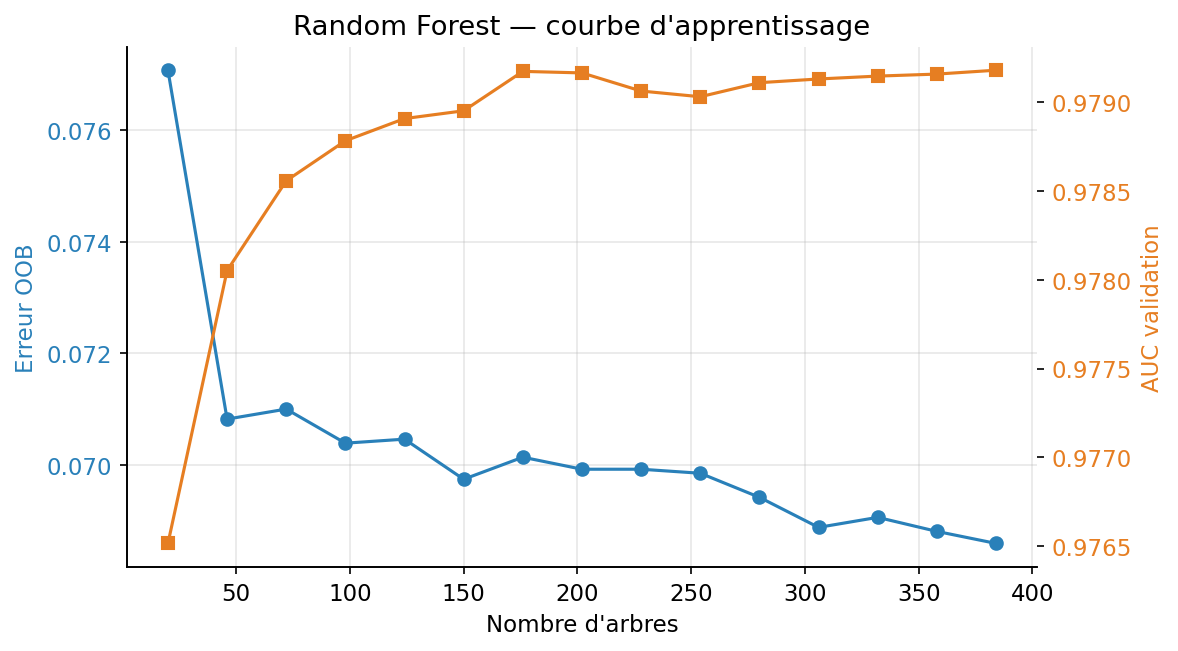
\includegraphics[width=0.82\linewidth]{Chap3/images/figures/fig04_rf_learning_curve.png}
    \caption{For\^et al\'eatoire~: erreur OOB (bleu, axe gauche) et AUC de validation (orange, axe droit) selon le nombre d'arbres.}
    \label{fig:rf-lc}
\end{figure}

On observe que l'erreur OOB d\'ecro\^it rapidement puis se stabilise autour de 0,069 (score OOB = 0,931), tandis que l'AUC de validation progresse dans la m\^eme direction et atteint un plateau~; la convergence de ces deux indicateurs ind\'ependants confirme que le mod\`ele g\'en\'eralise sans surapprentissage.

La figure~\ref{fig:xgb-lc} pr\'esente la courbe d'apprentissage de XGBoost~: la perte sur l'entra\^inement et l'AUC sur la validation sont suivies \`a chaque it\'eration de boosting, un arr\^et anticip\'e (\emph{early stopping}) interrompant l'entra\^inement si la validation ne s'am\'eliore plus pendant 50 it\'erations cons\'ecutives.

\begin{figure}[H]
    \centering
    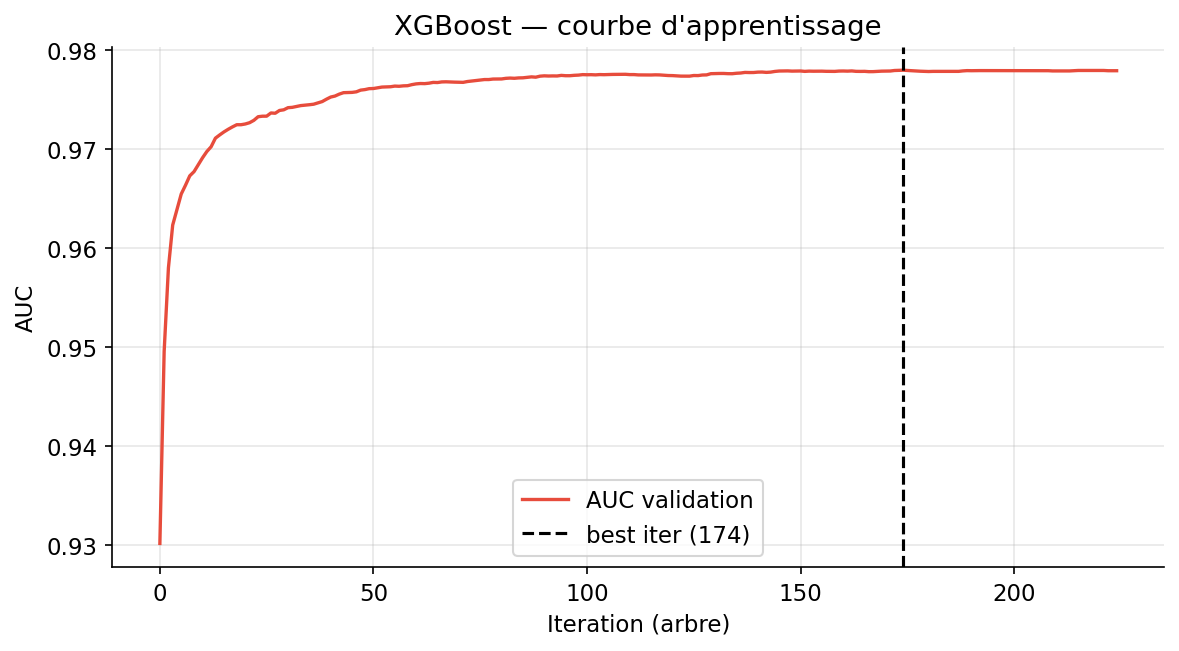
\includegraphics[width=0.82\linewidth]{Chap3/images/figures/fig09_xgb_learning_curve.png}
    \caption{XGBoost~: \'evolution de la perte d'entra\^inement et de l'AUC de validation selon le nombre d'it\'erations de boosting~; la ligne verticale indique l'it\'eration retenue par arr\^et anticip\'e.}
    \label{fig:xgb-lc}
\end{figure}

On observe que la perte d'entra\^inement d\'ecro\^it r\'eguli\`erement tandis que l'AUC de validation se stabilise rapidement~; l'arr\^et anticip\'e s\'electionne l'it\'eration~174 sur les 1\,900 disponibles, ce qui montre que le mod\`ele converge bien avant d'\'epuiser son budget et qu'il n'est pas sous-param\'etr\'e.

\mySubSection{Mod\`ele relationnel~: HGT}{}
\label{sec:contrib-hgt}

Le c\oe ur du second volet est un transformeur de graphe h\'et\'erog\`ene (HGT), dont le principe a \'et\'e pr\'esent\'e \`a la section~\ref{sec:hgt}~; nous en d\'ecrivons ici l'instanciation propre \`a la pr\'ediction PFAS. Le graphe repose sur de v\'eritables entit\'es partag\'ees plut\^ot que sur des attributs recopi\'es (figure~\ref{fig:schema4}). Les n\oe uds \texttt{sample} repr\'esentent les pr\'el\`evements, sans aucune variable de localisation. Trois types de n\oe uds-relais portent le contexte spatial~: les sites de contamination (\texttt{source}), les sous-bassins hydrog\'eologiques (\texttt{subbasin}) et des clusters g\'eographiques obtenus par KMeans (\texttt{geo\_cluster}). Des ar\^etes \texttt{near\_geo} relient directement les pr\'el\`evements \`a leurs plus proches voisins spatiaux. Deux forages proches d'un m\^eme site ou d'un m\^eme sous-bassin \'echangent ainsi de l'information. Pour \'eviter toute fuite, clusters, voisinages et sous-bassins sont construits \`a l'int\'erieur de chaque partition.

\begin{figure}[H]
    \centering
    
\includegraphics[width=0.9\linewidth]{Chap3/images/mermaid/schema4.png}
    \caption{Graphe h\'et\'erog\`ene relationnel~: les n\oe uds \texttt{sample} ne portent aucune variable de localisation~; ils sont reli\'es \`a des entit\'es partag\'ees (\texttt{source}, \texttt{subbasin}, \texttt{geo\_cluster}) et entre eux par des ar\^etes spatiales \texttt{near\_geo}.}
    \label{fig:schema4}
\end{figure}

Le HGT propage l'information le long des ar\^etes par un m\'ecanisme d'attention propre \`a chaque type de relation~: un n\oe ud \texttt{sample} agr\`ege diff\'eremment les messages venus d'un site, d'un sous-bassin ou d'un voisin spatial (figure~\ref{fig:schema5}). Apr\`es plusieurs couches, chaque pr\'el\`evement dispose d'un vecteur de repr\'esentation qui r\'esume son contexte relationnel et alimente un classifieur final. L'entra\^inement s'\'etend sur 300 \'epoques avec optimisation Optuna~; deux techniques d'augmentation r\'egularisent le mod\`ele~: l'ajout de bruit gaussien sur les variables des n\oe uds et le retrait al\'eatoire d'ar\^etes (DropEdge)~; le mod\`ele retenu est celui qui maximise le F1 sur la validation.

\begin{figure}[H]
    \centering
    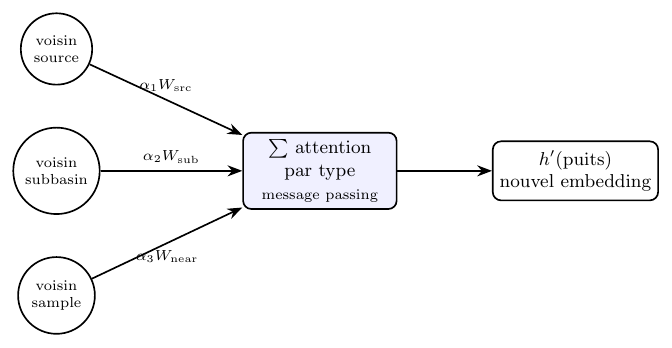
\includegraphics[width=0.9\linewidth]{Chap3/images/latex/schema5.png}
    \caption{M\'ecanisme d'une couche HGT~: passage de message et attention propre \`a chaque type d'ar\^ete, sur le voisinage d'un forage.}
    \label{fig:schema5}
\end{figure}

La figure~\ref{fig:hgt-lc} pr\'esente la courbe d'apprentissage du HGT~: perte d'entra\^inement et F1 de validation sont suivis sur les 300 \'epoques. Optuna a retenu une architecture \`a une seule couche de convolution (\texttt{num\_layers = 1}), ce qui limite la propagation de l'information \`a un saut dans le graphe~: chaque forage agr\`ege uniquement ses voisins directs, sans acc\`es \`a des informations de second rang.

\begin{figure}[H]
    \centering
    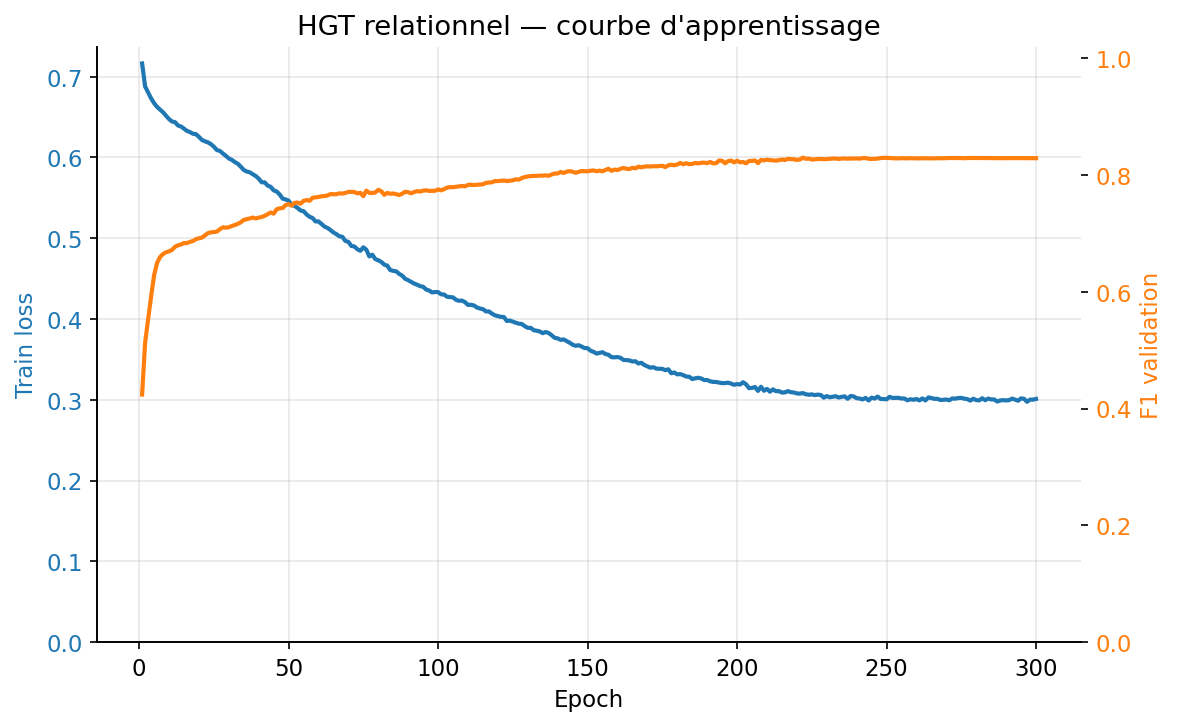
\includegraphics[width=0.82\linewidth]{Chap3/images/figures/fig14_hgt_learning_curve.png}
    \caption{HGT relationnel~: perte d'entra\^inement (axe gauche, bleu) et F1 de validation (axe droit, orange) selon l'\'epoque~; le mod\`ele retenu est celui qui maximise le F1 sur la validation.}
    \label{fig:hgt-lc}
\end{figure}

On observe que la convergence est lente~: le F1 de validation d\'emarre \`a 0,42 \`a la premi\`ere \'epoque et n'atteint 0,78 qu'apr\`es la centaine d'\'epoques. La perte d'entra\^inement d\'ecro\^it r\'eguli\`erement sans diverger, signe que le graphe apprend un signal r\'eel, mais \`a une vitesse et un niveau de performance sensiblement inf\'erieurs \`a ceux des mod\`eles tabulaires.

\mySubSection{Mod\`eles hybrides}{}
\label{sec:contrib-hybrides}

Deux mod\`eles cherchent \`a combiner le meilleur des deux familles.

La \textbf{fusion par embeddings} extrait le vecteur de repr\'esentation (128 dimensions) appris par le HGT pour chaque forage, le compresse par ACP en 2 composantes capturant 97~\% de la variance, puis concat\`ene ces deux composantes aux 97 variables tabulaires. La matrice r\'esultante (99 colonnes) est fournie \`a un XGBoost optimis\'e ind\'ependamment. Ce mod\`ele teste si la repr\'esentation relationnelle du graphe apporte un compl\'ement aux variables de contexte d\'ej\`a pr\'esentes.

Le \textbf{stacking} repose sur un m\'eta-apprentissage en deux \'etapes (section~\ref{sec:stacking}). Les trois mod\`eles de base (RF, XGBoost, HGT) produisent, pour chaque forage, leurs probabilit\'es de d\'epassement~; ces sorties sont compl\'et\'ees par 19 m\'eta-caract\'eristiques~: probabilit\'es brutes, entropies, niveaux de confiance, produits et diff\'erences crois\'es entre mod\`eles, ainsi qu'une composante ACP des embeddings HGT. Un m\'eta-classifieur XGBoost, optimis\'e par Optuna, apprend \`a arbitrer entre les mod\`eles selon la configuration de ces m\'eta-caract\'eristiques.

\mySubSection{Protocole exp\'erimental}{}
\label{sec:contrib-protocole}

L'\'evaluation repose sur des m\'etriques adapt\'ees \`a une cible presque \'equilibr\'ee mais \`a enjeu asym\'etrique~: aire sous la courbe ROC et pr\'ecision moyenne pour le pouvoir de discrimination, rappel et pr\'ecision pour le compromis de d\'ecision, F1 et exactitude \'equilibr\'ee pour une synth\`ese. Chaque mod\`ele est optimis\'e par Optuna sur la validation, et sa robustesse est contr\^ol\'ee par une matrice de confusion. Le dispositif principal contre la m\'emorisation g\'eographique reste le retrait de la localisation des variables (section~\ref{sec:contrib-pretraitement}). La g\'en\'eralisation \`a des r\'egions non vues n'est pas test\'ee dans ce travail~: aucune validation crois\'ee spatiale par blocs n'a \'et\'e conduite, ce point \'etant discut\'e en section~\ref{sec:contrib-discussion}.


% =========================================================
\mySection{R\'esultats, interpr\'etabilit\'e et discussion}{}
\label{sec:contrib-resultats}
% =========================================================

Cette section rapporte les performances des cinq mod\`eles sur le jeu de test (9\,268 pr\'el\`evements, mode pr\'edictif), rend leurs d\'ecisions lisibles aux niveaux global et local, ouvre la bo\^ite noire du graphe, restitue les pr\'edictions sous forme cartographique, puis discute la port\'ee des r\'esultats.

\mySubSection{Performances compar\'ees}{}
\label{sec:contrib-perf}

Le tableau~\ref{tab:comparaison-modeles-chap3} r\'esume les performances sur le test. Les mod\`eles tabulaires dominent nettement~: la for\^et al\'eatoire et XGBoost atteignent une aire sous la courbe ROC proche de 0,98, et le stacking les \'egale sans les d\'epasser. Le HGT relationnel, qui ne re\c{c}oit la g\'eographie que par la structure du graphe, reste en retrait (ROC-AUC 0,906), la fusion se situant entre les deux familles.

\begin{table}[h!]
    \centering
    \caption{Performances compar\'ees des cinq mod\`eles sur le jeu de test (mode pr\'edictif, 9\,268 pr\'el\`evements). Meilleure valeur par colonne en gras.}
    \label{tab:comparaison-modeles-chap3}
    \begin{tabular}{lcccccc}
        \hline
        Mod\`ele & ROC-AUC & AP & Pr\'ecision & Rappel & F1 & Bal. Acc. \\
        \hline
        For\^et al\'eatoire & \textbf{0,979} & \textbf{0,976} & \textbf{0,930} & 0,920 & \textbf{0,925} & \textbf{0,931} \\
        Stacking         & 0,977 & 0,974 & 0,923 & \textbf{0,926} & 0,925 & 0,931 \\
        XGBoost          & 0,977 & 0,974 & 0,922 & 0,923 & 0,923 & 0,929 \\
        Fusion embeddings & 0,960 & 0,954 & 0,886 & 0,887 & 0,887 & 0,896 \\
        HGT relationnel  & 0,906 & 0,886 & 0,823 & 0,828 & 0,825 & 0,839 \\
        \hline
    \end{tabular}
\end{table}

La figure~\ref{fig:roc-pr-all} compl\`ete ce tableau par les courbes ROC et pr\'ecision-rappel des cinq mod\`eles.

\begin{figure}[H]
    \centering
    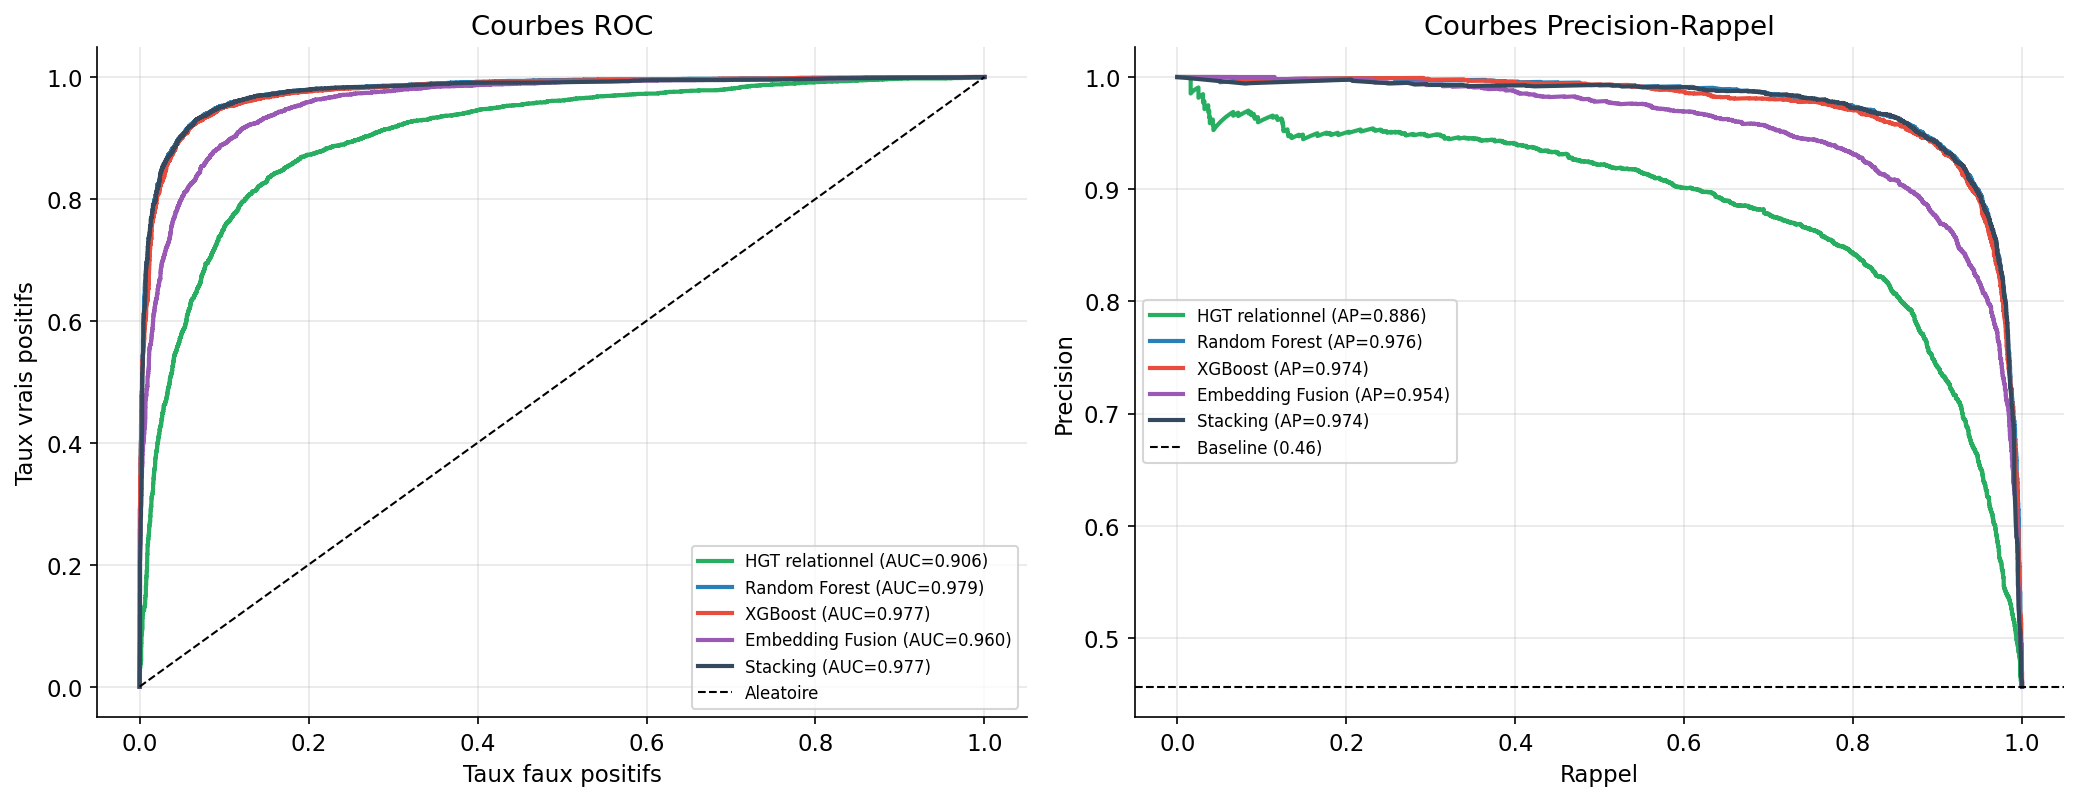
\includegraphics[width=0.95\linewidth]{Chap3/images/figures/fig24_roc_pr_all.png}
    \caption{Courbes ROC et pr\'ecision-rappel des cinq mod\`eles sur le jeu de test (mode pr\'edictif).}
    \label{fig:roc-pr-all}
\end{figure}
On observe que les trois mod\`eles \`a base d'arbres se superposent dans le coin sup\'erieur des deux courbes, tandis que le HGT relationnel forme une courbe nettement plus basse~: structurer la g\'eographie dans un graphe capte un signal r\'eel mais plus pauvre que les variables de contexte. Trois constats se d\'egagent. D'abord, retirer la localisation des variables n'effondre pas les mod\`eles tabulaires, qui restent tr\`es performants en s'appuyant sur les variables issues de \texttt{geoenrich}. Ensuite, structurer la g\'eographie dans un graphe ne suffit pas \`a \'egaler ces variables de contexte. Enfin, les hybrides ne tirent pas profit du relationnel~: la fusion dilue l\'eg\`erement la performance tabulaire et le stacking se contente d'\'egaler la for\^et al\'eatoire, signe d'une faible compl\'ementarit\'e entre les familles. La figure~\ref{fig:dashboard} en donne une vue synth\'etique.

\begin{figure}[H]
    \centering
    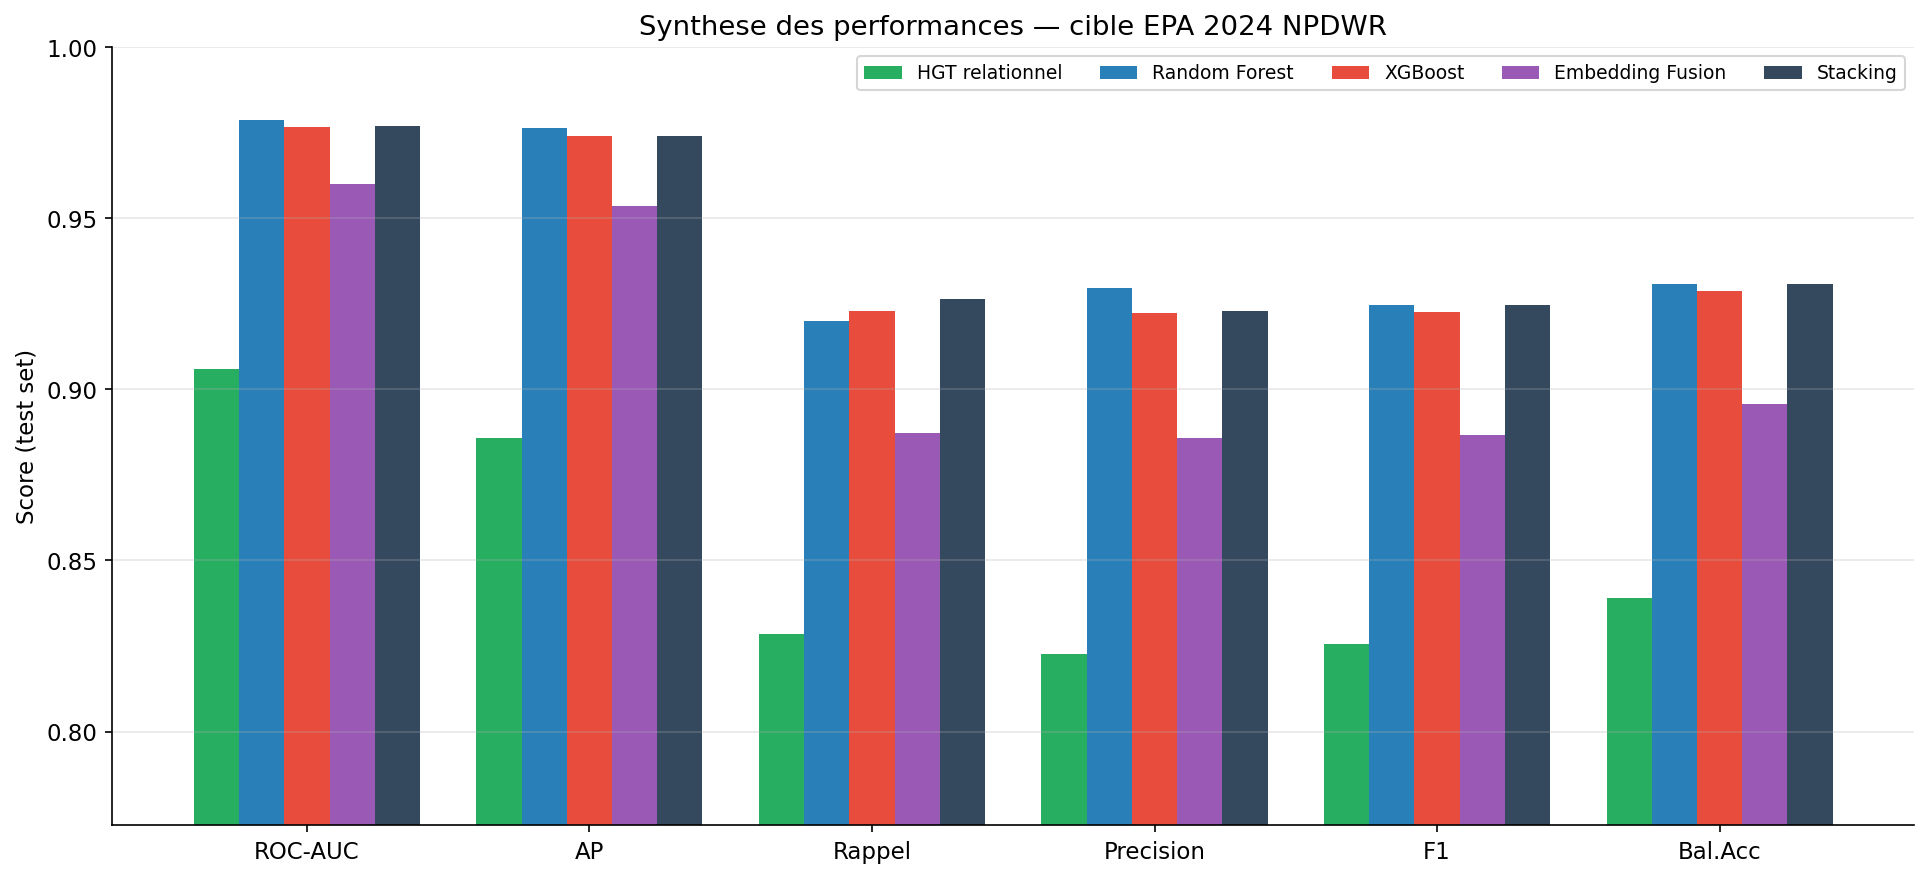
\includegraphics[width=0.95\linewidth]{Chap3/images/figures/fig27_dashboard.png}
    \caption{Tableau de bord comparatif des cinq mod\`eles (m\'etriques et matrices de confusion sur le jeu de test).}
    \label{fig:dashboard}
\end{figure}
On constate que les \'ecarts de F1 et d'exactitude \'equilibr\'ee confirment le classement~: l'architecture la plus \'elabor\'ee n'est pas la plus performante sur ce jeu.

Au-del\`a des m\'etriques de discrimination, un outil destin\'e \`a prioriser des forages \`a contr\^oler doit produire des probabilit\'es fiables~: si le mod\`ele annonce un risque de 70~\%, ce risque doit se r\'ealiser pour environ 70~\% des puits concern\'es. La figure~\ref{fig:calibration} confronte les probabilit\'es pr\'edites \`a la fr\'equence observ\'ee pour les cinq mod\`eles.

\begin{figure}[H]
    \centering
    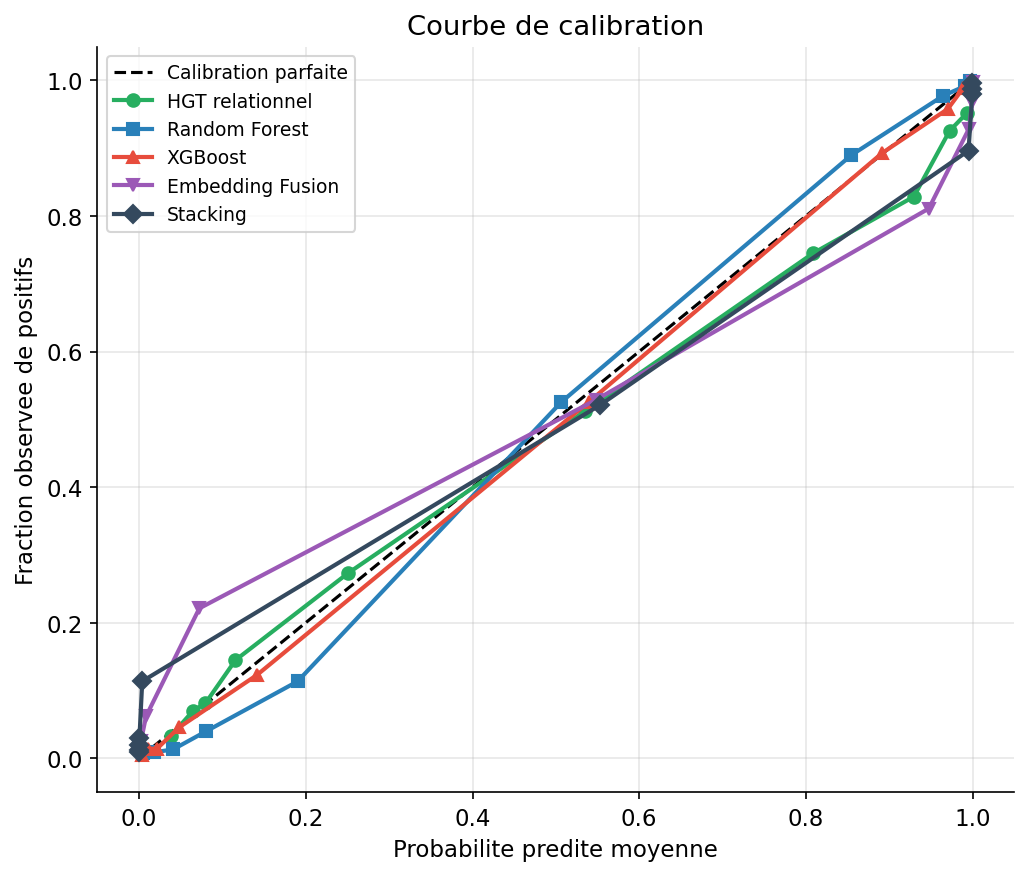
\includegraphics[width=0.82\linewidth]{Chap3/images/figures/fig25_calibration_all.png}
    \caption{Calibration des probabilit\'es de d\'epassement~: fr\'equence observ\'ee en fonction de la probabilit\'e pr\'edite pour les cinq mod\`eles (la diagonale repr\'esente une calibration parfaite).}
    \label{fig:calibration}
\end{figure}

On observe que la for\^et al\'eatoire et XGBoost, les plus performants en discrimination, pr\'esentent une calibration proche de la diagonale sur la majorit\'e de l'intervalle~; leurs probabilit\'es peuvent donc \^etre utilis\'ees directement pour classer des puits par ordre de risque d\'ecroissant. Le HGT et les mod\`eles hybrides s'en \'ecartent davantage, en particulier aux extr\'emit\'es, ce qui invite \`a les utiliser en classement relatif plut\^ot qu'en estimation absolue du risque. Pour un gestionnaire de surveillance, ce r\'esultat oriente le choix du mod\`ele~: la for\^et al\'eatoire offre le meilleur compromis entre discrimination et fiabilit\'e des probabilit\'es.

\mySubSection{Interpr\'etabilit\'e globale~: importance et concordance}{}
\label{sec:contrib-interp-globale}

L'analyse des importances de variables, men\'ee par valeurs de Shapley (section~\ref{sec:shapley-shap}), identifie les facteurs qui p\`esent le plus dans les pr\'edictions et mesure l'accord entre mod\`eles. Les variables les plus influentes sont la cat\'egorie du forage, la profondeur de la nappe, la densit\'e de sites de contamination dans le voisinage et la direction d'\'ecoulement. Ce sont des grandeurs de contexte hydrog\'eologique et de proximit\'e aux sources, et non des coordonn\'ees, ce qui est coh\'erent avec le retrait de la localisation. La figure~\ref{fig:importance} compare les importances par mod\`ele et la figure~\ref{fig:concordance} la concordance des rangs.

\begin{figure}[H]
    \centering
    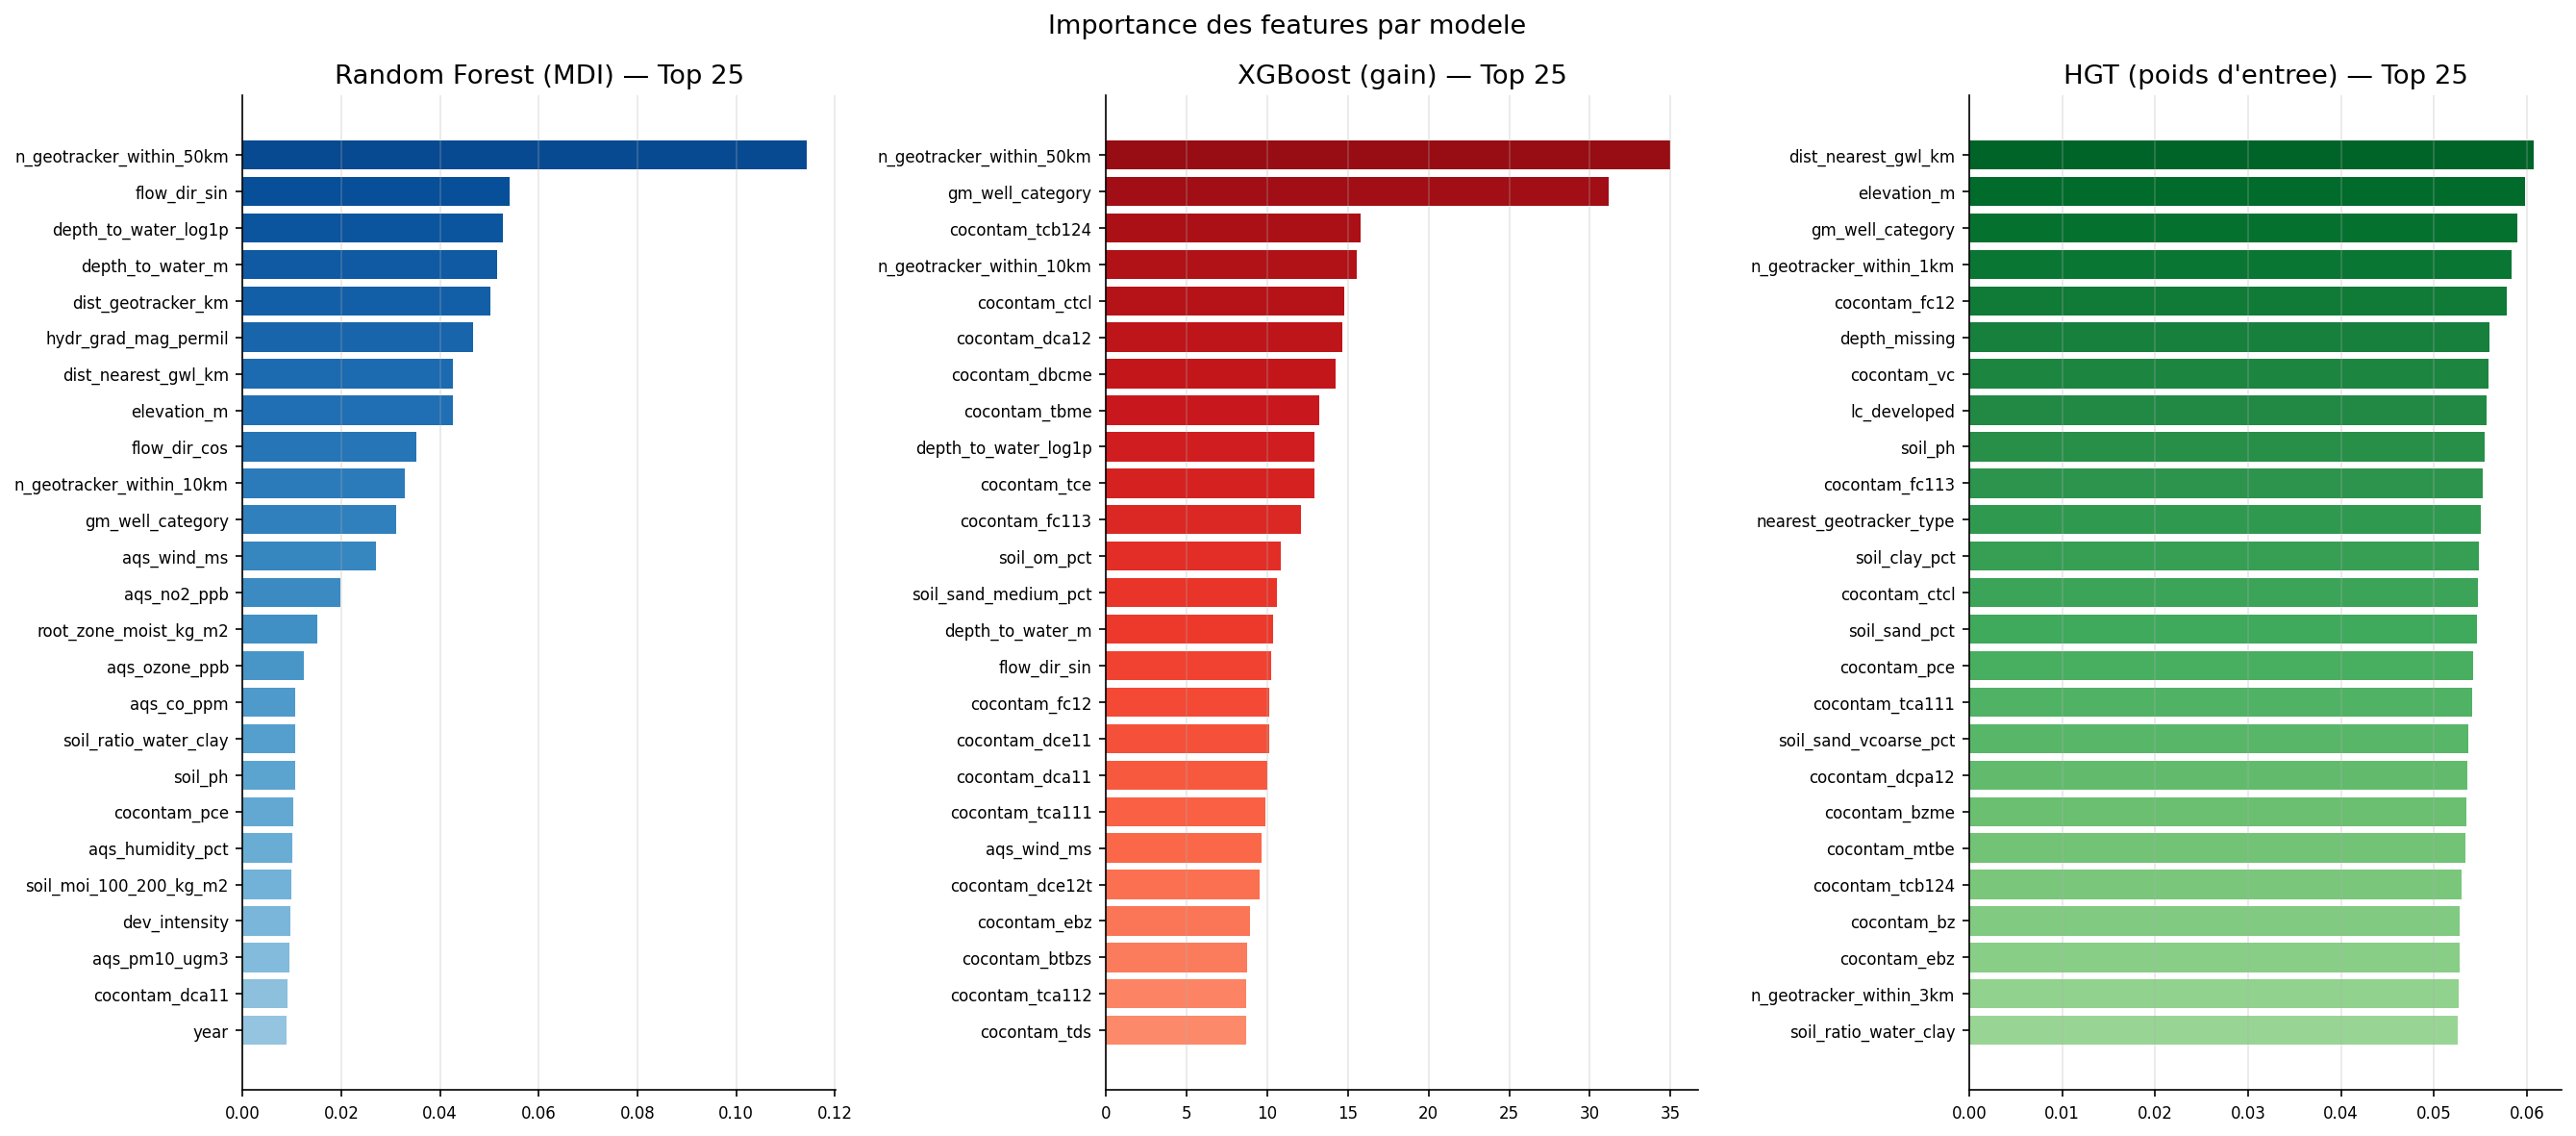
\includegraphics[width=0.95\linewidth]{Chap3/images/figures/fig40_importance_par_modele.png}
    \caption{Importance des variables par mod\`ele (Top 25, valeurs de Shapley).}
    \label{fig:importance}
\end{figure}

\begin{figure}[H]
    \centering
    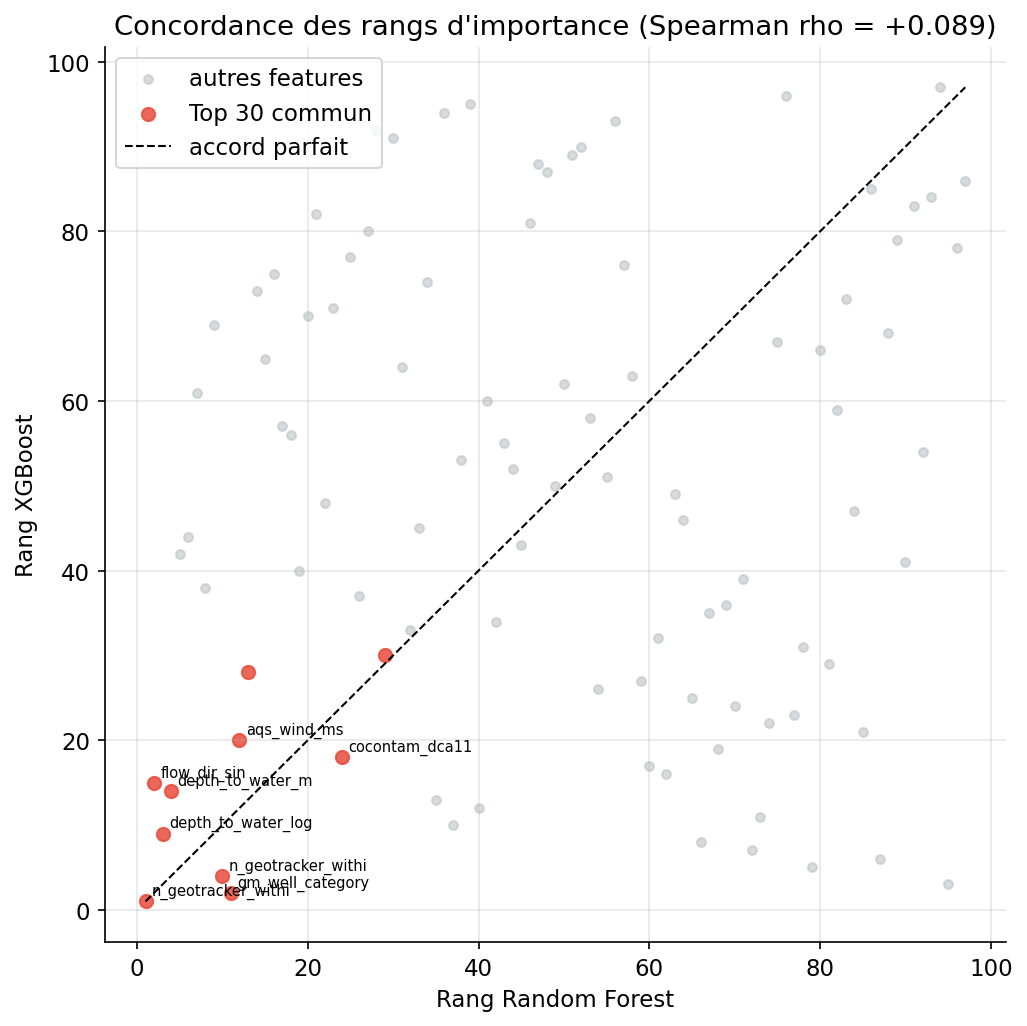
\includegraphics[width=0.75\linewidth]{Chap3/images/figures/fig41_concordance_rangs.png}
    \caption{Concordance des rangs d'importance entre mod\`eles.}
    \label{fig:concordance}
\end{figure}
On observe que les variables les plus influentes pour les mod\`eles tabulaires sont \texttt{n\_geotracker\_within\_50km} (rang~1 pour RF et XGBoost), la cat\'egorie du forage (\texttt{gm\_well\_category}, rang~2 pour XGBoost, rang~3 pour le HGT) et la profondeur de la nappe (\texttt{depth\_to\_water\_m}, rang~4 pour RF)~: pour un d\'ecideur, ces trois variables de proximit\'e et de contexte hydrog\'eologique constituent les facteurs diagnostiques prioritaires.

La concordance inter-mod\`eles, mesur\'ee par le coefficient de Spearman sur les rangs d'importance (Top~30), r\'ev\`ele un r\'esultat contre-intuitif. RF et XGBoost, pourtant presque aussi performants (AUC 0,979 vs 0,977), s'accordent tr\`es peu~: $\rho = 0{,}09$, avec seulement 10 variables communes. Deux mod\`eles presque \'equiperformants s'appuient donc sur des hi\'erarchies de variables sensiblement diff\'erentes. La paire XGBoost/HGT pr\'esente paradoxalement la concordance la plus \'elev\'ee ($\rho = 0{,}39$, avec 12 variables communes), alors que leurs performances respectives sont les plus \'eloign\'ees du banc. La concordance RF/HGT est la plus faible ($\rho = 0{,}05$, avec 7 variables communes). Ces chiffres indiquent que les trois mod\`eles lisent le probl\`eme par des canaux structurellement diff\'erents~; que cette diversit\'e ne se traduise pas en gain de stacking est un constat important, sugg\'erant que les canaux sont redondants plut\^ot que compl\'ementaires.

\mySubSection{Interpr\'etabilit\'e locale}{}
\label{sec:contrib-interp-locale}

Au-del\`a des tendances globales, chaque mod\`ele est expliqu\'e au niveau d'une pr\'ediction individuelle, sur un forage positif et un forage n\'egatif, par d\'ecomposition de la d\'ecision en contributions de variables (section~\ref{sec:shap-global-local}). Ces explications locales montrent quelles caract\'eristiques d'un forage ont pouss\'e la d\'ecision vers le d\'epassement ou vers la conformit\'e, ce qui rend une pr\'ediction d\'efendable aupr\`es d'un d\'ecideur, sans pour autant valoir preuve de causalit\'e. Nous illustrons ici l'interpr\'etabilit\'e locale sur la for\^et al\'eatoire, meilleur mod\`ele du banc.

La figure~\ref{fig:shap-local-rf-pos} d\'ecompose la d\'ecision pour un forage class\'e \`a risque~: chaque barre repr\'esente la contribution d'une variable (valeur de Shapley) \`a l'\'ecart entre la probabilit\'e pr\'edite et la probabilit\'e de r\'ef\'erence.

\begin{figure}[H]
    \centering
    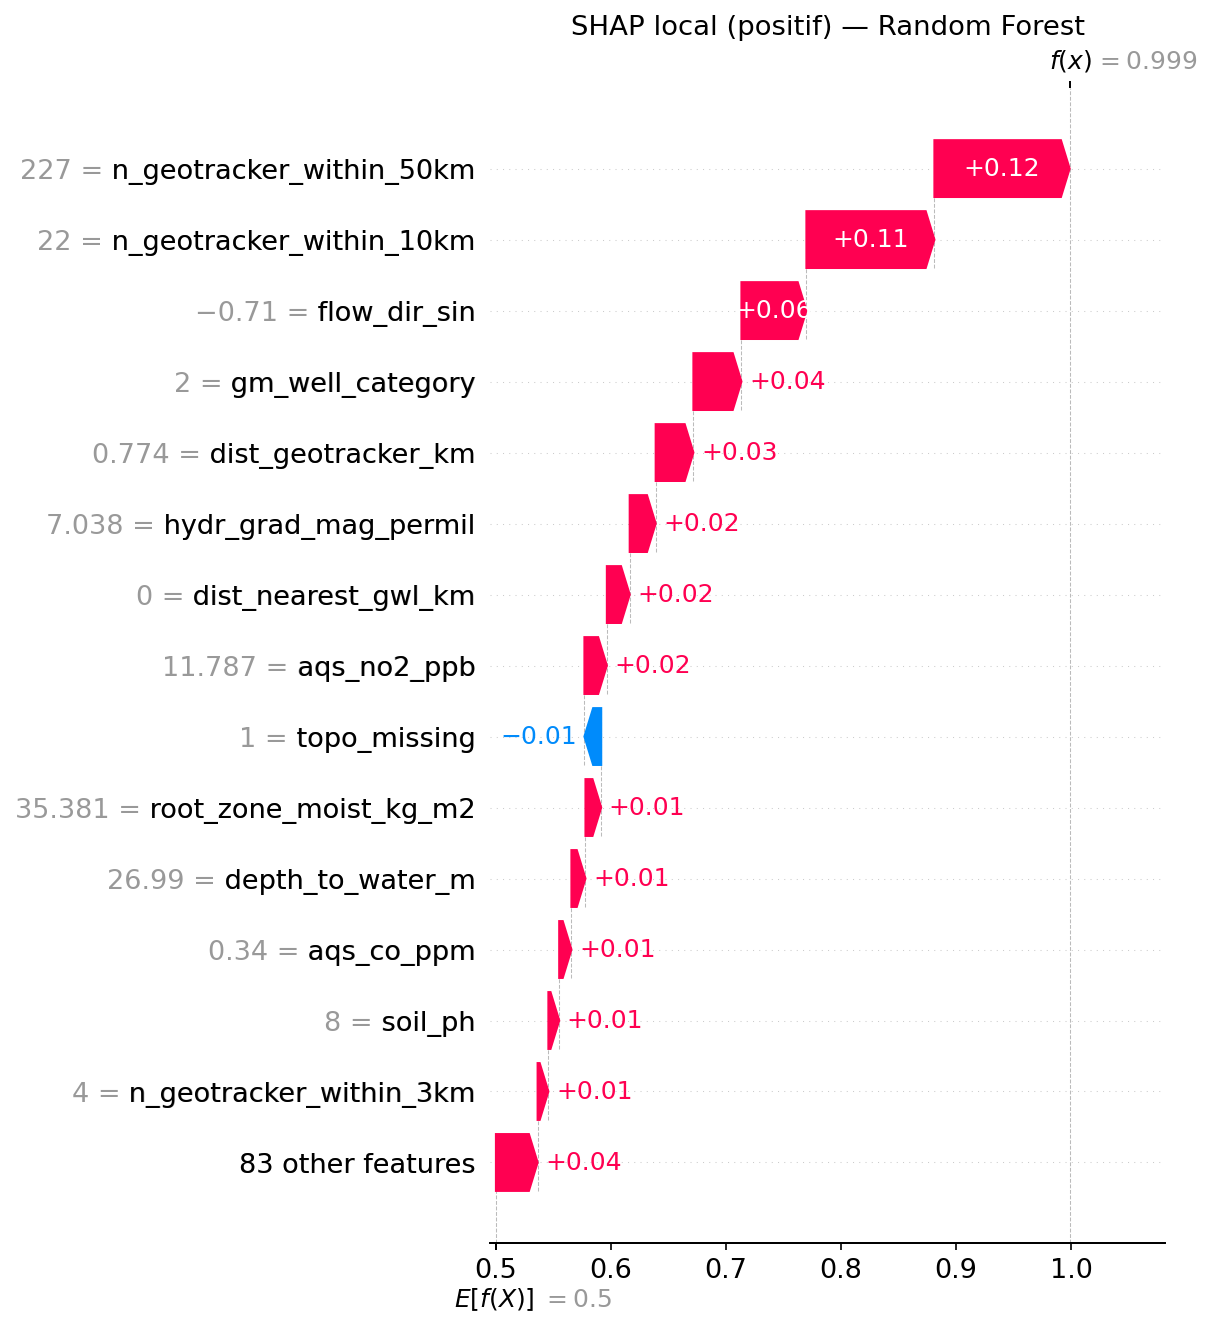
\includegraphics[width=0.85\linewidth]{Chap3/images/figures/fig06b_shap_local_rf_positif.png}
    \caption{Explication locale SHAP (diagramme \emph{waterfall}) de la for\^et al\'eatoire pour un forage class\'e \`a risque.}
    \label{fig:shap-local-rf-pos}
\end{figure}

On observe que la pr\'ediction est port\'ee par la densit\'e \'elev\'ee de sites de contamination \`a proximit\'e (\texttt{n\_geotracker\_within\_50km}), combin\'ee \`a la profondeur de la nappe et \`a la direction d'\'ecoulement~; ces variables accumulent la quasi-totalit\'e de la contribution positive et sont coh\'erentes avec les m\'ecanismes hydrog\'eologiques de migration des PFAS.

La figure~\ref{fig:shap-local-rf-neg} pr\'esente le cas sym\'etrique, un forage pr\'edit conforme.

\begin{figure}[H]
    \centering
    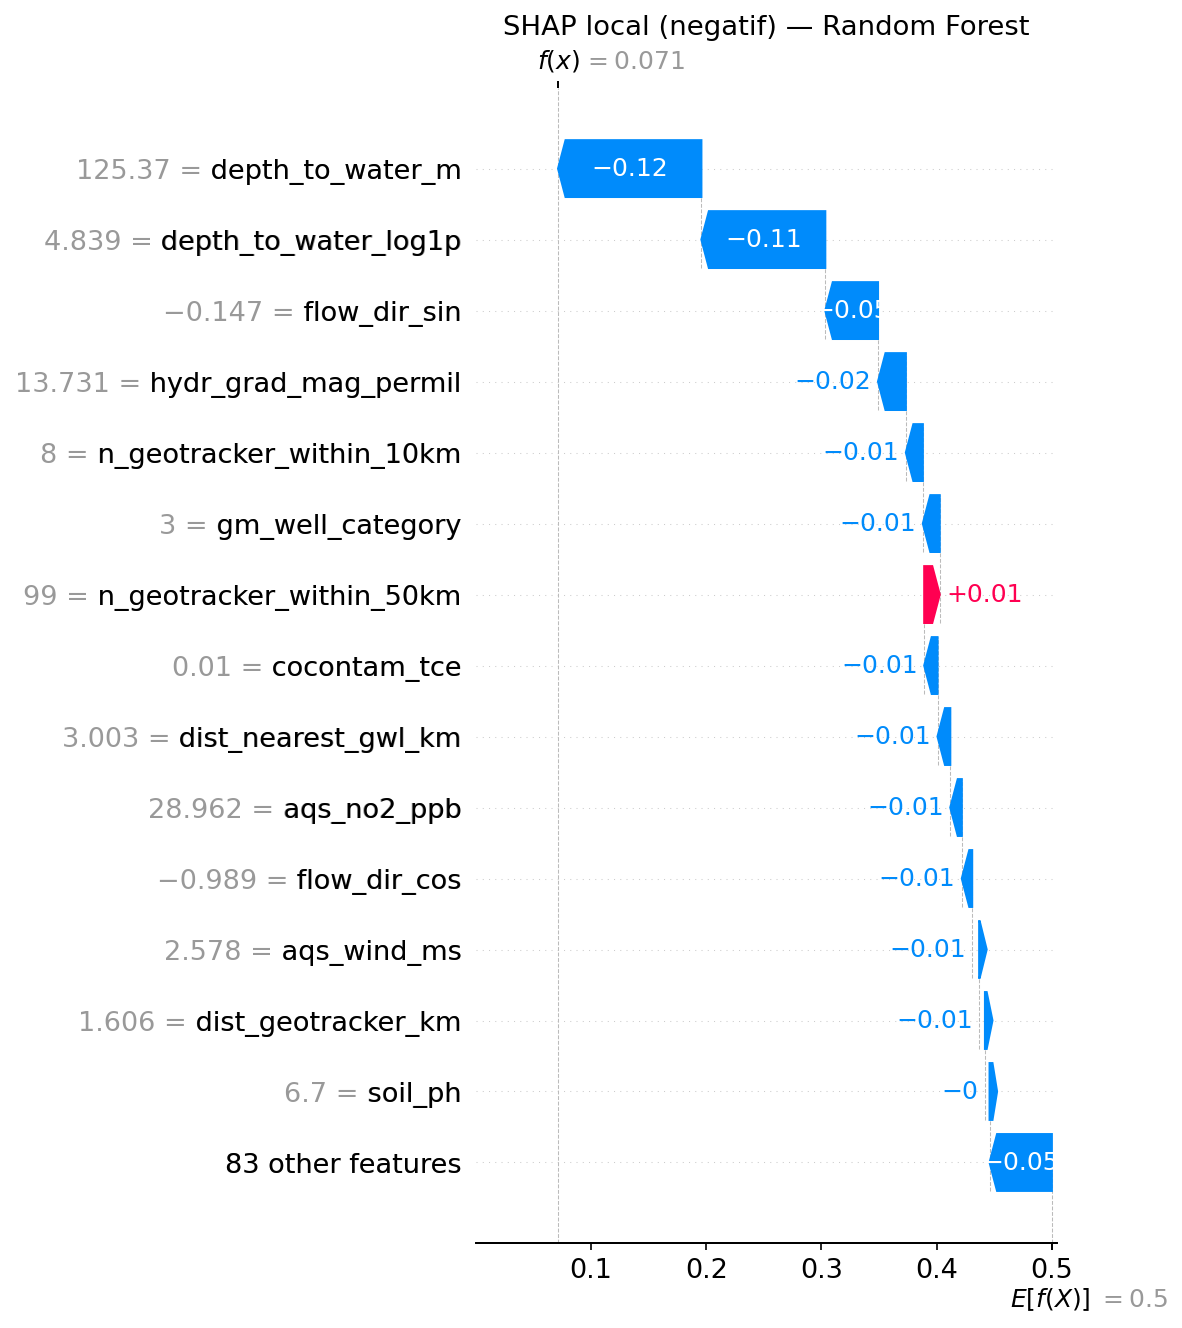
\includegraphics[width=0.85\linewidth]{Chap3/images/figures/fig06b_shap_local_rf_negatif.png}
    \caption{Explication locale SHAP (diagramme \emph{waterfall}) de la for\^et al\'eatoire pour un forage class\'e conforme.}
    \label{fig:shap-local-rf-neg}
\end{figure}

On constate que les m\^emes variables jouent dans le sens inverse~: la faible densit\'e de sites \`a proximit\'e et une profondeur de nappe \'elev\'ee sont les arguments principaux en faveur de la conformit\'e. La coh\'erence des facteurs d\'eterminants entre les deux cas renforce la cr\'edibilit\'e du mod\`ele~: ses d\'ecisions s'appuient sur des grandeurs physiquement interpr\'etables, ce qui est une condition n\'ecessaire pour en faire un outil d'aide \`a la priorisation de la surveillance.

\mySubSection{Sous le capot du HGT}{}
\label{sec:contrib-hgt-capot}

\`A des fins p\'edagogiques, le fonctionnement du graphe relationnel est expos\'e pas \`a pas. Les figures~\ref{fig:site-neighborhood} et~\ref{fig:well-neighborhood} donnent \`a voir la structure h\'et\'erog\`ene effectivement construite autour d'un site de contamination puis d'un forage, et la figure~\ref{fig:embeddings-2d} projette en deux dimensions les embeddings appris.

\begin{figure}[H]
    \centering
    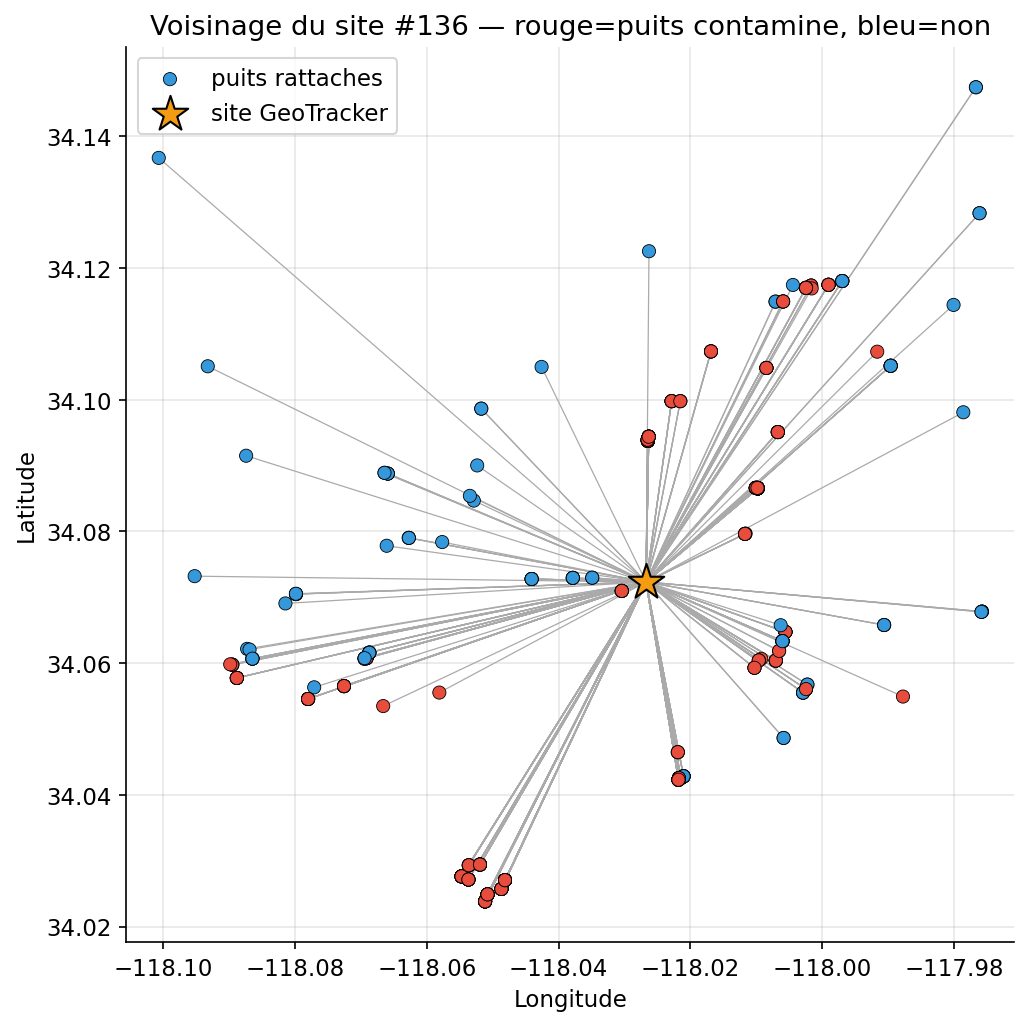
\includegraphics[width=0.8\linewidth]{Chap3/images/figures/fig30_site_neighborhood.png}
    \caption{Voisinage d'un site de contamination dans le graphe h\'et\'erog\`ene.}
    \label{fig:site-neighborhood}
\end{figure}

\begin{figure}[H]
    \centering
    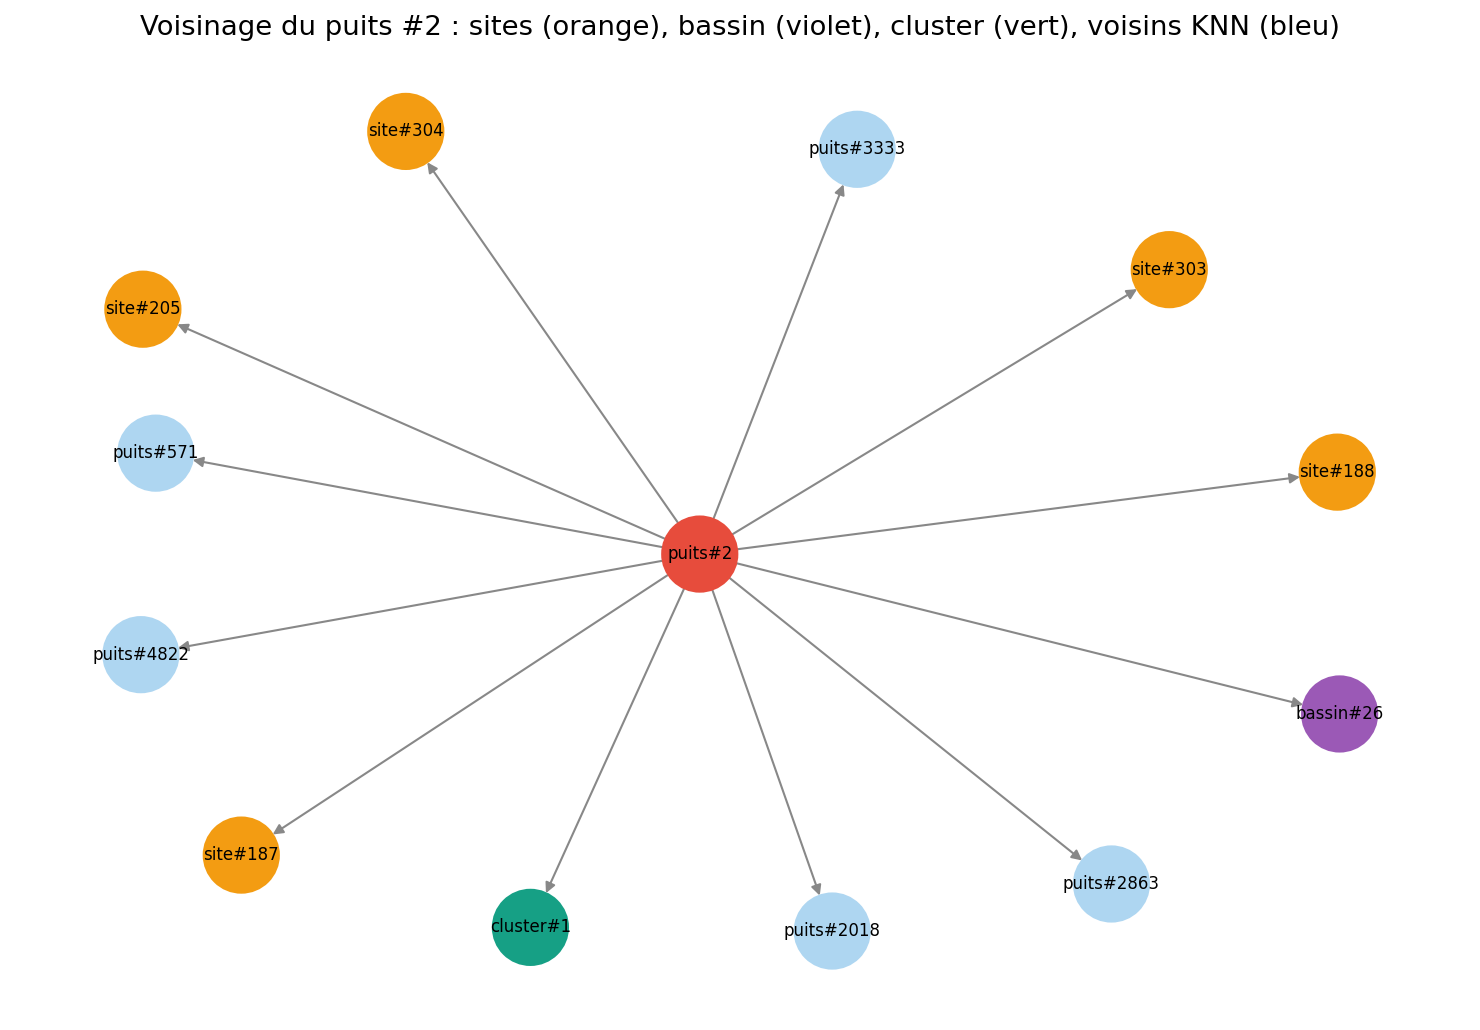
\includegraphics[width=0.8\linewidth]{Chap3/images/figures/fig31_well_neighborhood.png}
    \caption{Voisinage d'un forage~: ar\^etes vers les entit\'es partag\'ees et les voisins spatiaux.}
    \label{fig:well-neighborhood}
\end{figure}

\begin{figure}[H]
    \centering
    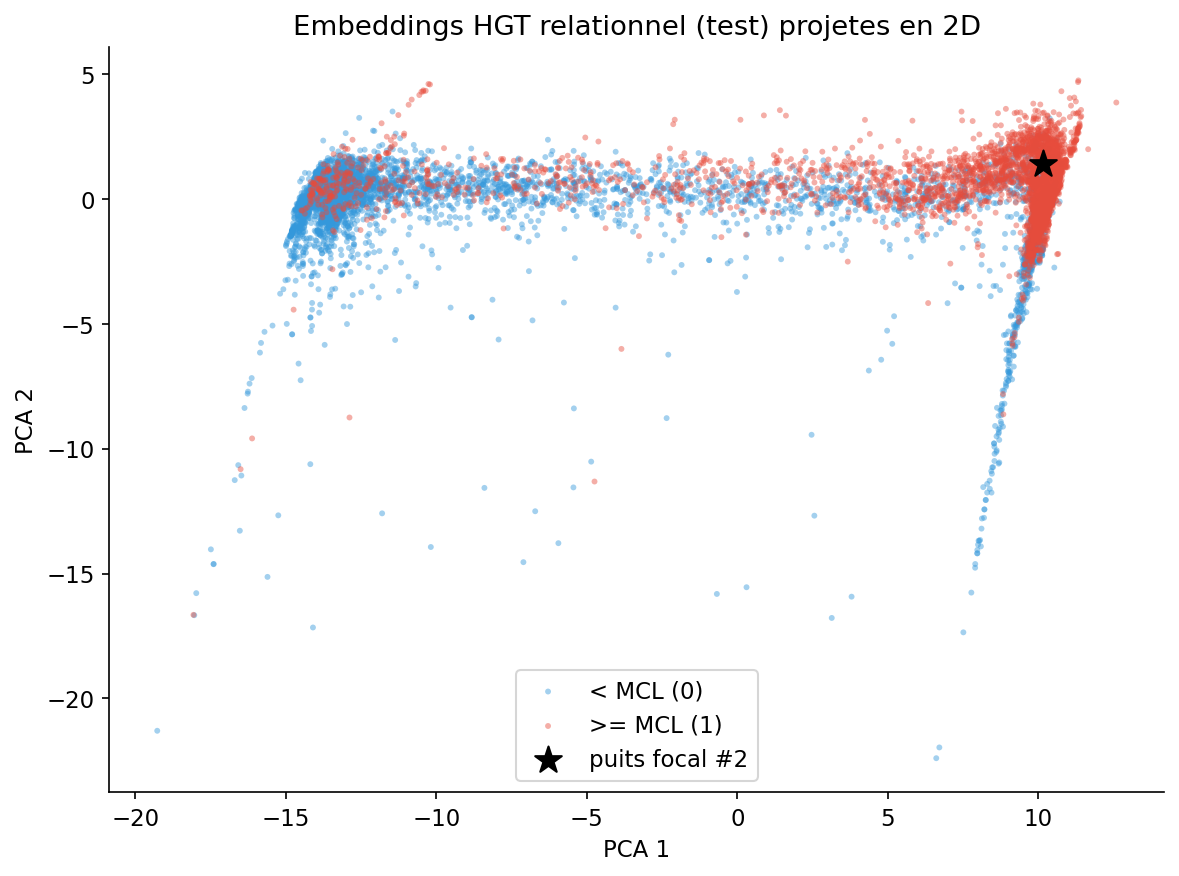
\includegraphics[width=0.8\linewidth]{Chap3/images/figures/fig33_hgt_embeddings_2d.png}
    \caption{Projection en deux dimensions des embeddings appris par le HGT, color\'ee par classe.}
    \label{fig:embeddings-2d}
\end{figure}
On observe que la projection s\'epare partiellement les forages \`a risque des autres~: la s\'eparation apprise est r\'eelle mais moins nette que celle que procurent les variables de contexte, ce qui explique le retrait du HGT en performance.

\mySubSection{Cartographie des pr\'edictions}{}
\label{sec:contrib-carte}

Les pr\'edictions du meilleur mod\`ele sont restitu\'ees spatialement (figure~\ref{fig:map-predictions}), ce qui permet de confronter les zones jug\'ees \`a risque \`a la g\'eographie connue de la contamination.

\begin{figure}[H]
    \centering
    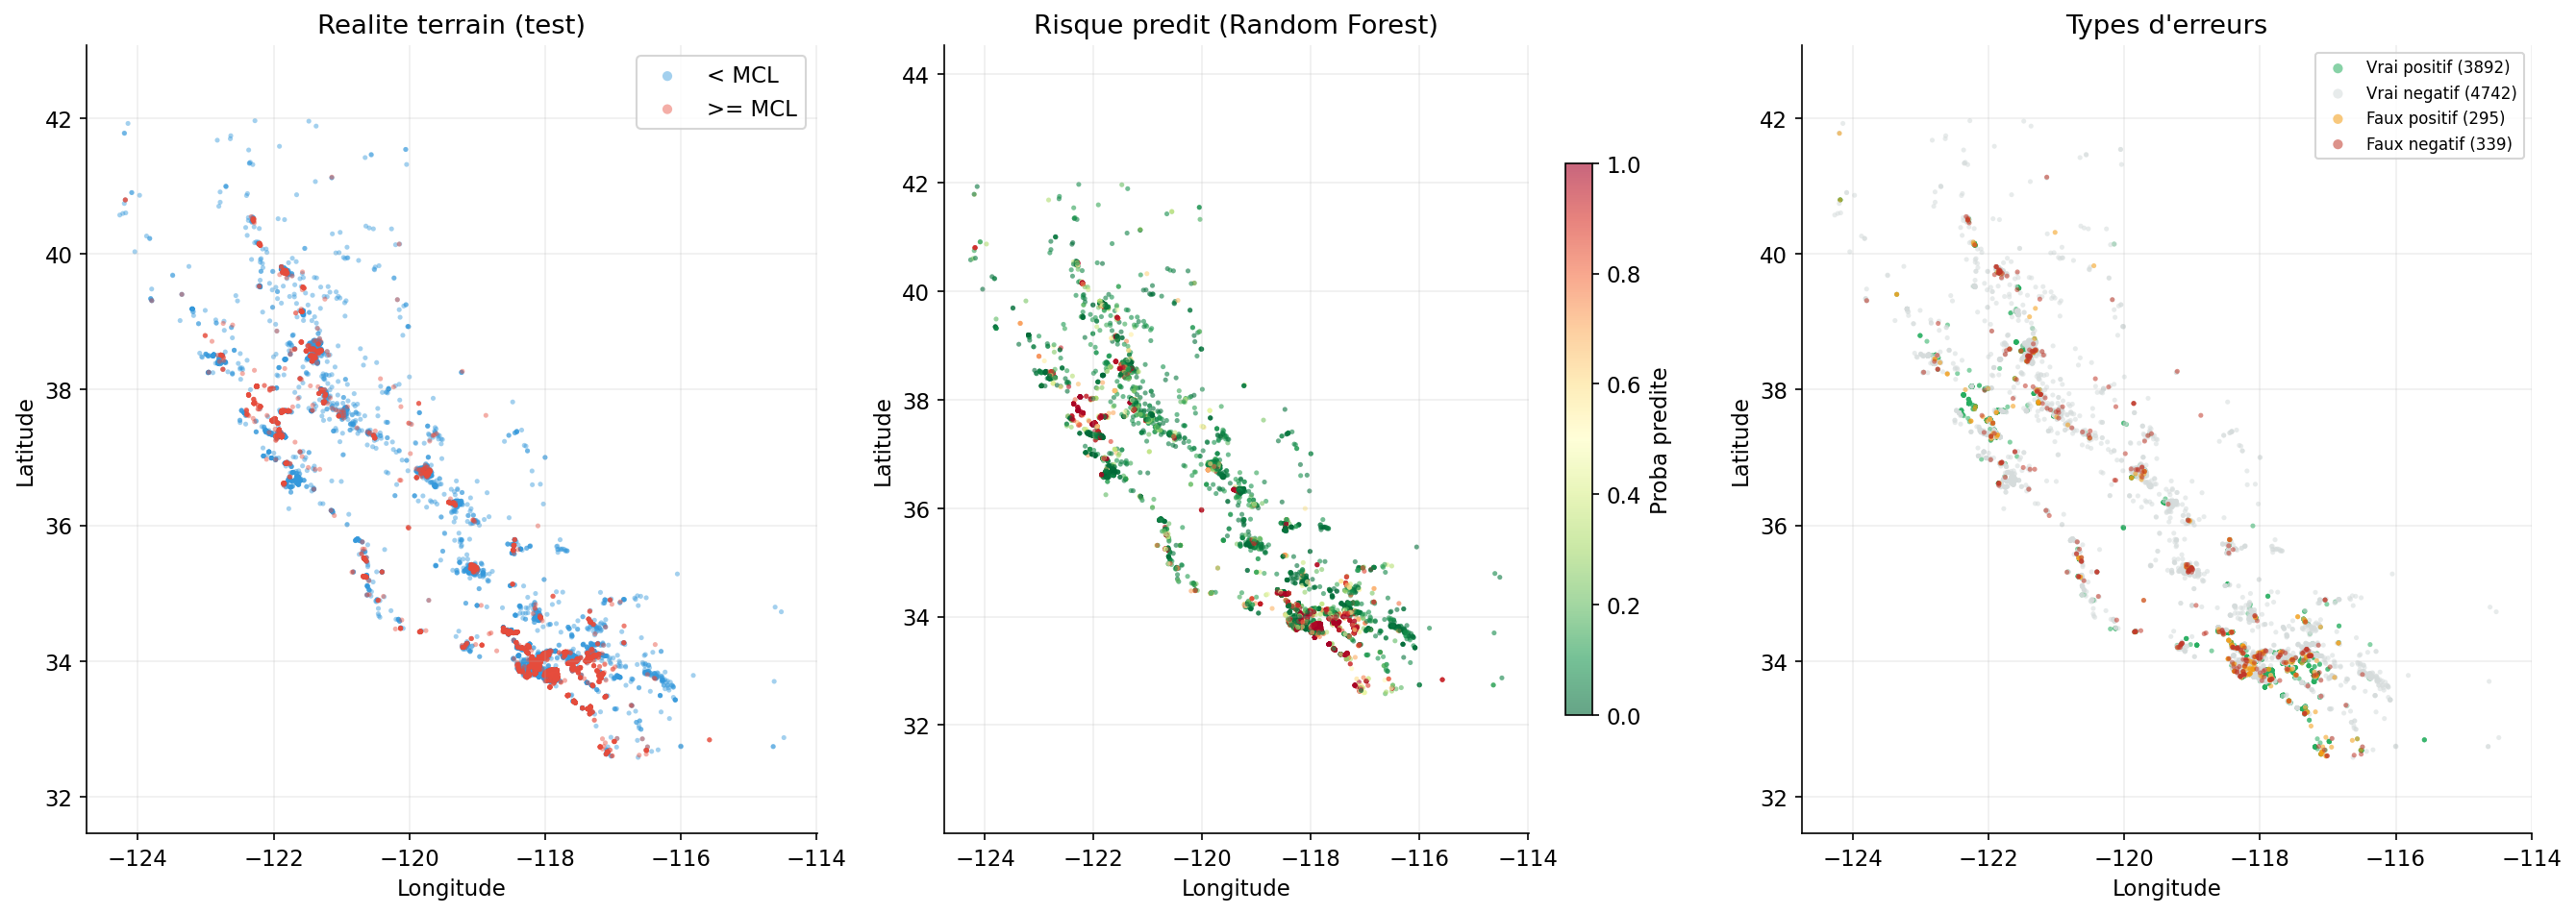
\includegraphics[width=0.8\linewidth]{Chap3/images/figures/fig28_map_predictions.png}
    \caption{Carte des pr\'edictions du meilleur mod\`ele sur la Californie.}
    \label{fig:map-predictions}
\end{figure}
On constate que les zones \`a risque pr\'edites co\"incident avec les secteurs historiquement contamin\'es, sans concentration manifeste de faux positifs, ce qui appuie l'usage du mod\`ele comme outil de priorisation de la surveillance.

\mySubSection{Discussion}{}
\label{sec:contrib-discussion}

Le principal enseignement est que, sur ce jeu de donn\'ees, les variables de contexte produites par \texttt{geoenrich} portent l'essentiel du signal pr\'edictif~: des mod\`eles tabulaires classiques, priv\'es de toute coordonn\'ee, atteignent une discrimination \'elev\'ee. Le pari de porter la g\'eographie par la structure d'un graphe plut\^ot que par des variables n'am\'eliore pas la pr\'ediction, et les hybrides ne d\'egagent pas de compl\'ementarit\'e exploitable. L'analyse des importances du m\'eta-classifieur du stacking le quantifie directement~: la probabilit\'e pr\'edite par le HGT (\texttt{hgt\_p1}) ne repr\'esente que 0,5~\% du poids d\'ecisionnel, contre 41~\% pour la probabilit\'e XGBoost et 7~\% pour celle de RF~; le produit crois\'e RF$\times$XGBoost (\texttt{prod\_xr}) concentre \`a lui seul 45~\% de l'importance. Le m\'eta-classifieur apprend donc \`a ignorer le HGT et \`a arbitrer presque exclusivement entre les deux mod\`eles tabulaires, ce qui explique que le stacking ne d\'epasse pas la for\^et al\'eatoire. Ce r\'esultat, n\'egatif au sens o\`u l'architecture la plus \'elabor\'ee n'est pas la plus performante, a sa valeur~: il montre qu'un enrichissement de contexte soign\'e peut rendre superflue une mod\'elisation relationnelle plus lourde.

Une limite m\'ethodologique m\'erite d'\^etre signal\'ee concernant les co-contaminants (\texttt{cocontam\_*}, 44 colonnes). Ces variables encodent la pr\'esence d'autres polluants mesur\'es dans les m\^emes programmes de surveillance que les PFAS~; or, les programmes de surveillance sont souvent d\'eclench\'es dans des zones d\'ej\`a suspect\'ees de contamination. Contrairement aux concentrations PFAS elles-m\^emes, les co-contaminants ne d\'efinissent pas la cible de fa\c{c}on d\'eterministe, mais ils peuvent en constituer un proxy indirect par biais de s\'election. Leur impact devra \^etre \'evalu\'e par une analyse de sensibilit\'e dans les travaux futurs.

Ces conclusions doivent \^etre temp\'er\'ees par une limite d'\'evaluation. Les performances rapport\'ees reposent sur un d\'ecoupage stratifi\'e al\'eatoire, qui ne teste pas la g\'en\'eralisation \`a des r\'egions enti\`erement non vues. Or la contamination PFAS est fortement auto-corr\'el\'ee dans l'espace, et m\^eme des variables de contexte (densit\'e de sites, proximit\'e) encodent indirectement la position~: une partie de la performance pourrait donc tenir \`a une auto-corr\'elation spatiale r\'esiduelle plut\^ot qu'\`a des m\'ecanismes transf\'erables. La validation crois\'ee spatiale par blocs est l'outil qui permettrait de mesurer ce risque, et son ex\'ecution constitue une priorit\'e pour consolider les conclusions. En l'absence de ce test, les comparaisons entre mod\`eles restent valides, puisqu'elles s'effectuent \`a protocole identique, mais le niveau absolu de performance doit \^etre interpr\'et\'e comme une borne sup\'erieure optimiste.

Par rapport \`a l'\'etat de l'art californien, Dong et al.~\cite{dong2024pfas} constituent la r\'ef\'erence la plus proche~: m\^eme corpus GAMA, m\^eme mode pr\'edictif strict (variables contextuelles exclusivement, sans concentration PFAS en entr\'ee). Deux diff\'erences structurelles emp\^echent toute comparaison chiffre \`a chiffre. D'une part, la cible change de cadre r\'eglementaire~: Dong et al. visent le seuil conjoint de 70~ng/L des recommandations EPA 2016, ce travail applique le NPDWR 2024 qui abaisse les seuils \`a 4~ng/L pour le PFOA et le PFOS et introduit le crit\`ere de m\'elange (HI)~; ce changement modifie la pr\'evalence des positifs et rend les m\'etriques non directement comparables. D'autre part, les paradigmes d'apprentissage diff\`erent~: Dong et al. mobilisent un pseudo-\'etiquetage semi-supervis\'e pour exploiter les 90~\% de puits sans analyse compl\`ete, et organisent la pr\'ediction en cha\^ine de classifieurs sur 35 analytes distincts~; ce travail est purement supervis\'e et formule la t\^ache comme un probl\`eme binaire unique sur la non-conformit\'e r\'eglementaire. L'apport architectural sp\'ecifique est l'introduction du HGT pour mod\'eliser la structure relationnelle spatiale entre forages, une direction absente de la litt\'erature PFAS publi\'ee (lacune~L1, section~\ref{sec:chap2-lacunes})~; les r\'esultats montrent que ce b\'en\'efice attendu ne s'est pas mat\'erialis\'e sur ce corpus, ce qui est en soi une information utile pour orienter de futurs travaux sur la structure relationnelle des r\'eseaux de surveillance.

% =========================================================
\mySection{Synth\`ese}{}
\label{sec:synthese-chap3}
% =========================================================

Ce chapitre a pr\'esent\'e une double contribution \`a la pr\'ediction du risque PFAS dans les eaux souterraines californiennes. La premi\`ere est un outil, \texttt{geoenrich}, moteur d'enrichissement g\'eospatial organis\'e en trois couches et fond\'e sur un contrat d'entr\'ee minimal qui s\'epare le \emph{o\`u/quand} universel de la charge utile \'etudi\'ee. Appliqu\'e \`a la base \texttt{wells\_pfas\_cleaned} reconstruite \`a partir des donn\'ees ouvertes californiennes (46\,338 pr\'el\`evements sur environ 11\,300 puits, d'avril 2016 \`a janvier 2026), il porte le jeu \`a 217 colonnes, dont les variables de contexte ajout\'ees par l'enrichissement spatial sont presque toutes compl\`etes (88 colonnes renseign\'ees \`a 100~\%). La seconde contribution est un banc de cinq mod\`eles, deux mod\`eles tabulaires de r\'ef\'erence, un transformeur de graphe h\'et\'erog\`ene et deux mod\`eles hybrides, \'evalu\'es \`a protocole identique et en mode pr\'edictif sur ce jeu enrichi.

L'enseignement principal est que les variables de contexte produites par \texttt{geoenrich} portent l'essentiel du signal pr\'edictif~: des mod\`eles tabulaires priv\'es de toute coordonn\'ee atteignent une discrimination \'elev\'ee (ROC-AUC proche de 0,98), tandis que structurer la g\'eographie dans un graphe relationnel n'am\'eliore pas la pr\'ediction et que les hybrides ne d\'egagent pas de compl\'ementarit\'e. Deux limites tracent les perspectives. D'une part, la r\'eutilisabilit\'e de \texttt{geoenrich} sur un autre polluant ou une autre r\'egion reste \`a confirmer par une application empirique \`a un nouveau jeu d'observations. D'autre part, l'\'evaluation repose sur un d\'ecoupage qui ne teste pas la g\'en\'eralisation \`a des zones non vues~; l'ex\'ecution de la validation crois\'ee spatiale par blocs est la priorit\'e imm\'ediate pour distinguer la part de signal transf\'erable de l'auto-corr\'elation spatiale r\'esiduelle. Ces deux chantiers prolongent le travail sans en remettre en cause les acquis~: un outil d'enrichissement r\'eutilisable et une comparaison rigoureuse et interpr\'etable de mod\`eles de pr\'ediction de la contamination.

	
	%Ainsi de suite
	
	%\myChapterStar{Titre}{Titre court}{Ajouter a la table des matieres? (false|true|chapter|section|subsection|subsubsection -chapter par defaut-)}
\myChapterStar{Conclusion g\'en\'erale}{}{true}
\label{chap:conclusion}
%\myMinitoc{Profondeur de la minitoc (section|subsection|subsubsection)}{Titre de la minitoc}
\myMiniToc{section}{Sommaire}

Ce m\'emoire a abord\'e la pr\'ediction du risque de d\'epassement r\'eglementaire PFAS dans les eaux souterraines en mode pr\'edictif strict, \`a partir de variables contextuelles g\'eospatiales seules et sans recours \`a des concentrations pr\'ealablement mesur\'ees. Nous rappelons ci-apr\`es la probl\'ematique et les choix m\'ethodologiques qui ont structur\'e ce travail, avant d'en analyser les r\'esultats de mani\`ere critique et de tracer les perspectives qu'ils ouvrent.

%\mySectionStar{Titre}{Titre court}{Ajouter a la table des matieres? (false|true|chapter|section|subsection|subsubsection -section par defaut-)}
\mySectionStar{Probl\'ematique \'etudi\'ee et choix m\'ethodologiques}{}{true}
\label{sec:concl-problematique}

La surveillance de la qualit\'e des eaux souterraines face \`a la contamination PFAS pose un d\'efi op\'erationnel concret~: l'analyse chimique par chromatographie liquide coupl\'ee \`a la spectrom\'etrie de masse co\^ute plusieurs centaines d'euros par \'echantillon, et les limites fix\'ees par l'EPA en 2024 dans le cadre de la r\'eglementation NPDWR descendent jusqu'\`a 4~ng/L pour le PFOA et le PFOS~\cite{epa2023npdwr}. Pr\'edire o\`u ces seuils sont susceptibles d'\^etre d\'epass\'es, sans concentration PFAS pr\'ealablement mesur\'ee, constitue donc un besoin r\'eel pour la priorisation des campagnes d'\'echantillonnage. Ce travail s'est attaqu\'e \`a ce probl\`eme sur un corpus de 46\,338 pr\'el\`evements d'eaux souterraines californiennes, constitu\'e en s'inspirant de la m\'ethodologie de collecte de Dong et al.~\cite{dong2024pfas}. Deux verrous ont structur\'e la d\'emarche.

Le premier est d'ordre logiciel. Toute approche de pr\'ediction g\'eospatiale suppose que les observations soient enrichies par des variables de contexte, telles que la proximit\'e des sources de contamination, les propri\'et\'es des sols et les variables hydrog\'eologiques, car ces caract\'eristiques sont absentes des jeux de donn\'ees PFAS bruts~\cite{dong2024pfas,george2021pfas}. Or cet enrichissement est g\'en\'eralement assur\'e par des scripts monolithiques, \'etroitement li\'es \`a un jeu de donn\'ees particulier et non r\'eutilisables. Pour lever ce verrou, nous avons con\c{c}u \texttt{geoenrich}, un moteur g\'en\'erique organis\'e en trois couches~: une couche \emph{contrat} agnostique, une couche \emph{op\'erateurs} rassemblant des primitives de jointure param\'etrables, et une couche \emph{configuration} qui concentre les choix propres \`a chaque r\'egion dans un fichier d\'eclaratif externe. Sa correction a \'et\'e \'etablie par un test de parit\'e avec le pipeline d'origine~: 77 colonnes strictement identiques, 17 mieux renseign\'ees et aucune r\'egression sur 94 colonnes produites.

Le second verrou est scientifique et tient \`a l'\'evaluation des mod\`eles. La contamination PFAS \'etant fortement auto-corr\'el\'ee dans l'espace~\cite{guelfo2021pfas}, un d\'ecoupage al\'eatoire train/test laisse des forages spatialement voisins de part et d'autre de la fronti\`ere, permettant \`a un mod\`ele de m\'emoriser la g\'eographie plut\^ot que d'apprendre des m\'ecanismes transf\'erables. Pour y r\'epondre, toute variable de localisation a \'et\'e retir\'ee des entr\'ees des mod\`eles~; les coordonn\'ees ne subsistent que dans la topologie du graphe relationnel construit pour le HGT. Cinq mod\`eles ont \'et\'e entra\^in\'es et compar\'es \`a protocole identique sur ce jeu enrichi~: deux mod\`eles tabulaires de r\'ef\'erence (for\^et al\'eatoire et XGBoost), un transformeur de graphe h\'et\'erog\`ene (HGT), et deux mod\`eles hybrides (Embedding Fusion et Stacking). Chacun a \'et\'e accompagn\'e d'analyses d'interpr\'etabilit\'e globale et locale par valeurs de Shapley~\cite{lundberg2017shap}.

\mySectionStar{Analyse critique des r\'esultats obtenus}{}{true}
\label{sec:concl-analyse}

Les r\'esultats obtenus sur le jeu de test, en mode pr\'edictif strict, montrent que les mod\`eles tabulaires dominent. La for\^et al\'eatoire et le stacking atteignent tous deux un score F1 de 0,925, avec des aires sous la courbe ROC de 0,979 et 0,977~; XGBoost suit de tr\`es pr\`es (F1 0,923, AUC 0,977). Le HGT relationnel, qui ne re\c{c}oit la g\'eographie que par la structure du graphe, reste nettement en retrait (F1 0,825, AUC 0,906), et la fusion par embeddings se situe entre les deux familles (F1 0,887, AUC 0,960). L'enseignement principal de cette comparaison est que les variables de contexte produites par \texttt{geoenrich}, m\^eme priv\'ees de coordonn\'ees, portent l'essentiel du signal pr\'edictif~: des mod\`eles tabulaires classiques atteignent une discrimination \'elev\'ee sans acc\`es \`a la localisation. Le graphe relationnel capte un signal r\'eel, mais il reste en retrait des mod\`eles tabulaires. Le stacking, arbitr\'e par un m\'eta-classifieur XGBoost, n'exploite pas la contribution du HGT et n'am\'eliore pas la for\^et al\'eatoire~: ce r\'esultat indique qu'un enrichissement de contexte soign\'e peut rendre superflue une mod\'elisation relationnelle plus lourde.

Ces conclusions doivent \^etre lues avec deux r\'eserves. La premi\`ere concerne l'\'evaluation~: les performances rapport\'ees reposent sur un d\'ecoupage strat\'ifi\'e al\'eatoire, qui ne teste pas la g\'en\'eralisation \`a des zones enti\`erement non vues. La contamination PFAS \'etant auto-corr\'el\'ee dans l'espace, une partie des scores pourrait tenir \`a une proximit\'e r\'esiduelle entre forages d'entra\^inement et de test plut\^ot qu'\`a des m\'ecanismes transf\'erables. Les chiffres obtenus constituent donc une borne sup\'erieure optimiste~; une validation crois\'ee spatiale par blocs permettrait de mesurer cet \'ecart. La seconde r\'eserve concerne \texttt{geoenrich}~: son ind\'ependance vis-\`a-vis du cas californien est \'etablie par inspection du code et par conception, mais la preuve empirique d\'ecisive reste \`a apporter. Ces deux limites ne remettent pas en cause la comparaison entre mod\`eles, qui s'effectue \`a protocole identique et demeure valide en termes relatifs.

L'analyse de l'interpr\'etabilit\'e globale par valeurs de Shapley confirme que les variables les plus influentes sont des grandeurs de contexte hydrog\'eologique et de proximit\'e aux sources (cat\'egorie du forage, profondeur de la nappe, densit\'e de sites de contamination dans le voisinage, direction d'\'ecoulement), et non des coordonn\'ees. Ce r\'esultat est coh\'erent avec le dispositif de retrait de la localisation et l\'egitime r\'etrospectivement la d\'ecision de ne pas fournir les coordonn\'ees comme variables d'entr\'ee.

\mySectionStar{Quelques perspectives}{}{true}
\label{sec:concl-perspectives}

Ce travail ouvre plusieurs directions de recherche et de d\'eveloppement que nous estimons prioritaires.

\begin{itemize}

    \item \textbf{Validation crois\'ee spatiale par blocs.} Cette validation n'a pas \'et\'e conduite dans le pr\'esent travail. Elle constitue la priorit\'e imm\'ediate~: elle permettrait de distinguer la part du signal pr\'edictif qui reste stable hors des zones d'entra\^inement de celle qui repose sur l'auto-corr\'elation spatiale r\'esiduelle, et de disposer ainsi d'une mesure honn\^ete de la transf\'erabilit\'e g\'eographique des mod\`eles.

    \item \textbf{D\'emonstration empirique de la g\'en\'ericit\'e de \texttt{geoenrich}.} L'ind\'ependance du moteur vis-\`a-vis du cas PFAS californien est \'etablie par construction. Convertir cette propri\'et\'e en preuve d\'emontr\'ee suppose de soumettre \`a l'outil un jeu d'observations portant sur un autre contaminant (nitrates, m\'etaux lourds, pesticides) ou une autre r\'egion, avec des couches de r\'ef\'erence adapt\'ees, et de v\'erifier que l'enrichissement produit est pertinent sans modifier une ligne du code du moteur. Ce test de g\'en\'eralit\'e consoliderait la contribution logicielle de ce m\'emoire.

    \item \textbf{Int\'egration de l'interpr\'etabilit\'e dans des outils d'aide \`a la d\'ecision.} Les explications locales par valeurs de Shapley~\cite{lundberg2017shap} permettent, pour chaque forage, d'identifier les facteurs qui ont orient\'e la pr\'ediction vers le d\'epassement ou vers la conformit\'e. Leur int\'egration dans un tableau de bord destin\'e aux gestionnaires de r\'eseaux d'eau rendrait les pr\'edictions lisibles et actionnables, en particulier pour la hi\'erarchisation des campagnes de contr\^ole analytique.

    \item \textbf{Application au Cameroun et au contexte africain.} La probl\'ematique pos\'ee par ce travail d\'epasse le cadre californien. Dans de nombreux pays africains, dont le Cameroun, les r\'eseaux de surveillance de la qualit\'e des eaux souterraines restent peu denses, et le recours syst\'ematique \`a l'analyse chimique des PFAS demeure hors de port\'ee budg\'etaire pour la plupart des gestionnaires. C'est pr\'ecis\'ement dans ces contextes de raret\'e des donn\'ees que le mode pr\'edictif strict pr\'esente le plus de valeur~: il ne requiert aucune concentration PFAS pr\'ealable et s'appuie uniquement sur le contexte g\'eospatial (proximit\'e des sites militaires et industriels ayant utilis\'e des mousses anti-incendie AFFF, propri\'et\'es des sols, variables hydrog\'eologiques). \texttt{geoenrich} a \'et\'e con\c{c}u pour \^etre r\'egion-agnostique~: assembler les couches de r\'ef\'erence pertinentes \`a partir de bases mondiales (ISRIC SoilGrids pour les sols, bases de donn\'ees hydrog\'eologiques continentales, registres de sites industriels nationaux) suffirait, en principe, \`a l'instancier pour un contexte camerounais ou africain. Une telle extension supposerait de collecter un \'echantillon de mesures de calibration sur le terrain, de constituer les couches de r\'ef\'erence correspondantes et de valider le pipeline dans ce nouvel environnement. Les r\'esultats obtenus sur le dataset californien constituent un point de d\'epart encourageant pour envisager cette transposition.

\end{itemize}


\myCleanStarChapterEnd

	
	%************ Bibliographie ***************
	% La charte de l'�cole doctorale recommande un style dans lequel les citations seront de la forme (NomAuteur, Ann�e) ou (NomAuteur et al., Ann�e)
	%\myBibliography{style}{url du fichier .bib}
	\myBibliography{vancouver}{bibliography}
	
	% *********** Annexes *********************
	\appendix
	
	\myChapter{Hyperparam\`etres des mod\`eles}{Hyperparam\`etres des mod\`eles}\label{ann:hyperparams}
\mySaveMarks

Cette annexe d\'etaille les espaces de recherche explor\'es par Optuna pour les trois mod\`eles de base~: la for\^et al\'eatoire (RF), XGBoost et le transformeur de graphe h\'et\'erog\`ene (HGT). Pour chaque hyperparam\`etre, on indique le type de suggestion utilis\'e par le cadre TPE (\emph{Tree-structured Parzen Estimator}), l'intervalle ou les valeurs candidates, la valeur de d\'epart inject\'ee en premier essai, et la \textbf{valeur retenue} par Optuna \`a l'issue de l'optimisation (run complet, mode \texttt{FULL}). Les param\`etres fix\'es, non soumis \`a l'optimisation, sont list\'es \`a part.

% ---------------------------------------------------------
\mySectionStar{For\^et al\'eatoire}{}{false}
\label{ann:hyp-rf}
% ---------------------------------------------------------

\begin{table}[H]
    \centering
    \small
    \caption{Espace de recherche et valeur retenue par Optuna pour la for\^et al\'eatoire (AUC-CV\,=\,0,971).}
    \label{tab:hyp-rf}
    \begin{tabular}{lllll}
        \hline
        Hyperparam\`etre & Type & Intervalle / valeurs & D\'epart & \textbf{Retenu} \\
        \hline
        \texttt{n\_estimators}       & entier   & $[200, 800]$, pas 100              & 500           & \textbf{400}  \\
        \texttt{max\_depth}          & cat\'eg. & \texttt{None}, 15, 20, 30          & \texttt{None} & \textbf{20}   \\
        \texttt{max\_features}       & cat\'eg. & \texttt{sqrt}, \texttt{log2}, 0.3, 0.5 & \texttt{sqrt} & \textbf{0.5} \\
        \texttt{min\_samples\_leaf}  & entier   & $[1, 10]$                          & 2             & \textbf{2}    \\
        \texttt{min\_samples\_split} & entier   & $[2, 15]$                          & 2             & \textbf{2}    \\
        \hline
    \end{tabular}
\end{table}

Param\`etres fix\'es~: \texttt{class\_weight = "balanced"} (correction du d\'es\'equilibre r\'esiduel), \texttt{oob\_score = True} (contr\^ole hors-sac), \texttt{n\_jobs = -1}, \texttt{random\_state} fix\'e.

% ---------------------------------------------------------
\mySectionStar{XGBoost}{}{false}
\label{ann:hyp-xgb}
% ---------------------------------------------------------

\begin{table}[H]
    \centering
    \small
    \caption{Espace de recherche et valeur retenue par Optuna pour XGBoost (AUC-val\,=\,0,978).}
    \label{tab:hyp-xgb}
    \begin{tabular}{lllll}
        \hline
        Hyperparam\`etre & Type & Intervalle & D\'epart & \textbf{Retenu} \\
        \hline
        \texttt{n\_estimators}      & entier        & $[200, 2000]$, pas 100 & 1000  & \textbf{1900}                  \\
        \texttt{learning\_rate}     & flottant (log) & $[0.005, 0.3]$        & 0.05  & \textbf{0.0775}                \\
        \texttt{max\_depth}         & entier        & $[3, 12]$              & 6     & \textbf{12}                    \\
        \texttt{subsample}          & flottant      & $[0.5, 1.0]$           & 0.8   & \textbf{1.00}                  \\
        \texttt{colsample\_bytree}  & flottant      & $[0.4, 1.0]$           & 0.8   & \textbf{0.81}                  \\
        \texttt{min\_child\_weight} & entier        & $[1, 15]$              & 3     & \textbf{3}                     \\
        \texttt{gamma}              & flottant      & $[0.0, 2.0]$           & 0.1   & \textbf{0.23}                  \\
        \texttt{reg\_alpha}         & flottant (log) & $[10^{-8}, 10]$       & 0.1   & $\mathbf{3.2 \times 10^{-5}}$  \\
        \texttt{reg\_lambda}        & flottant (log) & $[10^{-8}, 10]$       & 1.0   & $\mathbf{2.3 \times 10^{-2}}$  \\
        \hline
    \end{tabular}
\end{table}

Param\`etres fix\'es~: \texttt{tree\_method = "hist"} (histogramme, plus rapide sur grands jeux), \texttt{scale\_pos\_weight} calcul\'e comme le rapport des effectifs (classe n\'egative sur classe positive), \texttt{early\_stopping\_rounds = 50} sur l'AUC de validation, \texttt{eval\_metric = "auc"}, \texttt{random\_state} fix\'e.

% ---------------------------------------------------------
\mySectionStar{Transformeur de graphe h\'et\'erog\`ene (HGT)}{}{false}
\label{ann:hyp-hgt}
% ---------------------------------------------------------

\begin{table}[H]
    \centering
    \small
    \caption{Espace de recherche et valeur retenue par Optuna pour le HGT (F1-val maximis\'e).}
    \label{tab:hyp-hgt}
    \begin{tabular}{lllll}
        \hline
        Hyperparam\`etre  & Type           & Intervalle / valeurs       & D\'epart            & \textbf{Retenu}               \\
        \hline
        \texttt{hidden\_channels} & cat\'eg. & 32, 64, 128              & 64                  & \textbf{128}                  \\
        \texttt{num\_heads}       & cat\'eg. & 2, 4                     & 4                   & \textbf{2}                    \\
        \texttt{num\_layers}      & entier   & $[1, 3]$                 & 2                   & \textbf{1}                    \\
        \texttt{dropout}          & flottant & $[0.1, 0.5]$             & 0.3                 & \textbf{0.17}                 \\
        \texttt{lr}               & flottant (log) & $[10^{-4}, 10^{-2}]$ & $3\times10^{-3}$  & $\mathbf{4.1\times10^{-4}}$   \\
        \texttt{weight\_decay}    & flottant (log) & $[10^{-5}, 10^{-3}]$ & $10^{-5}$          & $\mathbf{1.1\times10^{-4}}$   \\
        \hline
    \end{tabular}
\end{table}

Param\`etres fix\'es~: \texttt{epochs = 300}, optimiseur Adam, crit\`ere d'arr\^et sur le F1 de validation (le mod\`ele retenu est celui de la meilleure \'epoque). L'augmentation comprend un bruit gaussien sur les attributs des n\oe uds et un retrait al\'eatoire d'ar\^etes (\emph{DropEdge}) \`a chaque passe d'entra\^inement.

\myRestoreMarks

	% \myChapter{Publication issue de ce travail}{Publication issue de ce travail}\label{ann:publication}
\mySaveMarks

Cette annexe reproduit l'article de conf\'erence co-\'ecrit lors de ces travaux et accept\'e \`a la conf\'erence IEEE International Conference on Bioinformatics and Biomedicine (BIBM) 2025~\cite{bomgni2025pfas}.

\bigskip
\noindent\textbf{R\'ef\'erence~:} Bomgni, A.~B., Dnjomou~Yonmba, W.~L., T\'en\'e~Ceskouts\'e, R.~F., Klein, N., Gadhamshetty, V., et Gnimpieba, E.~Z. (2025). Heterogeneous Graph Network (HGN) for Binary Spatio-Chemical-Source Classification of Per- and Polyfluoroalkyl Substances (PFAS) Contamination: An Optimized Approach. \emph{2025 IEEE International Conference on Bioinformatics and Biomedicine (BIBM)}, pp.~2954--2958.

\clearpage
{\centering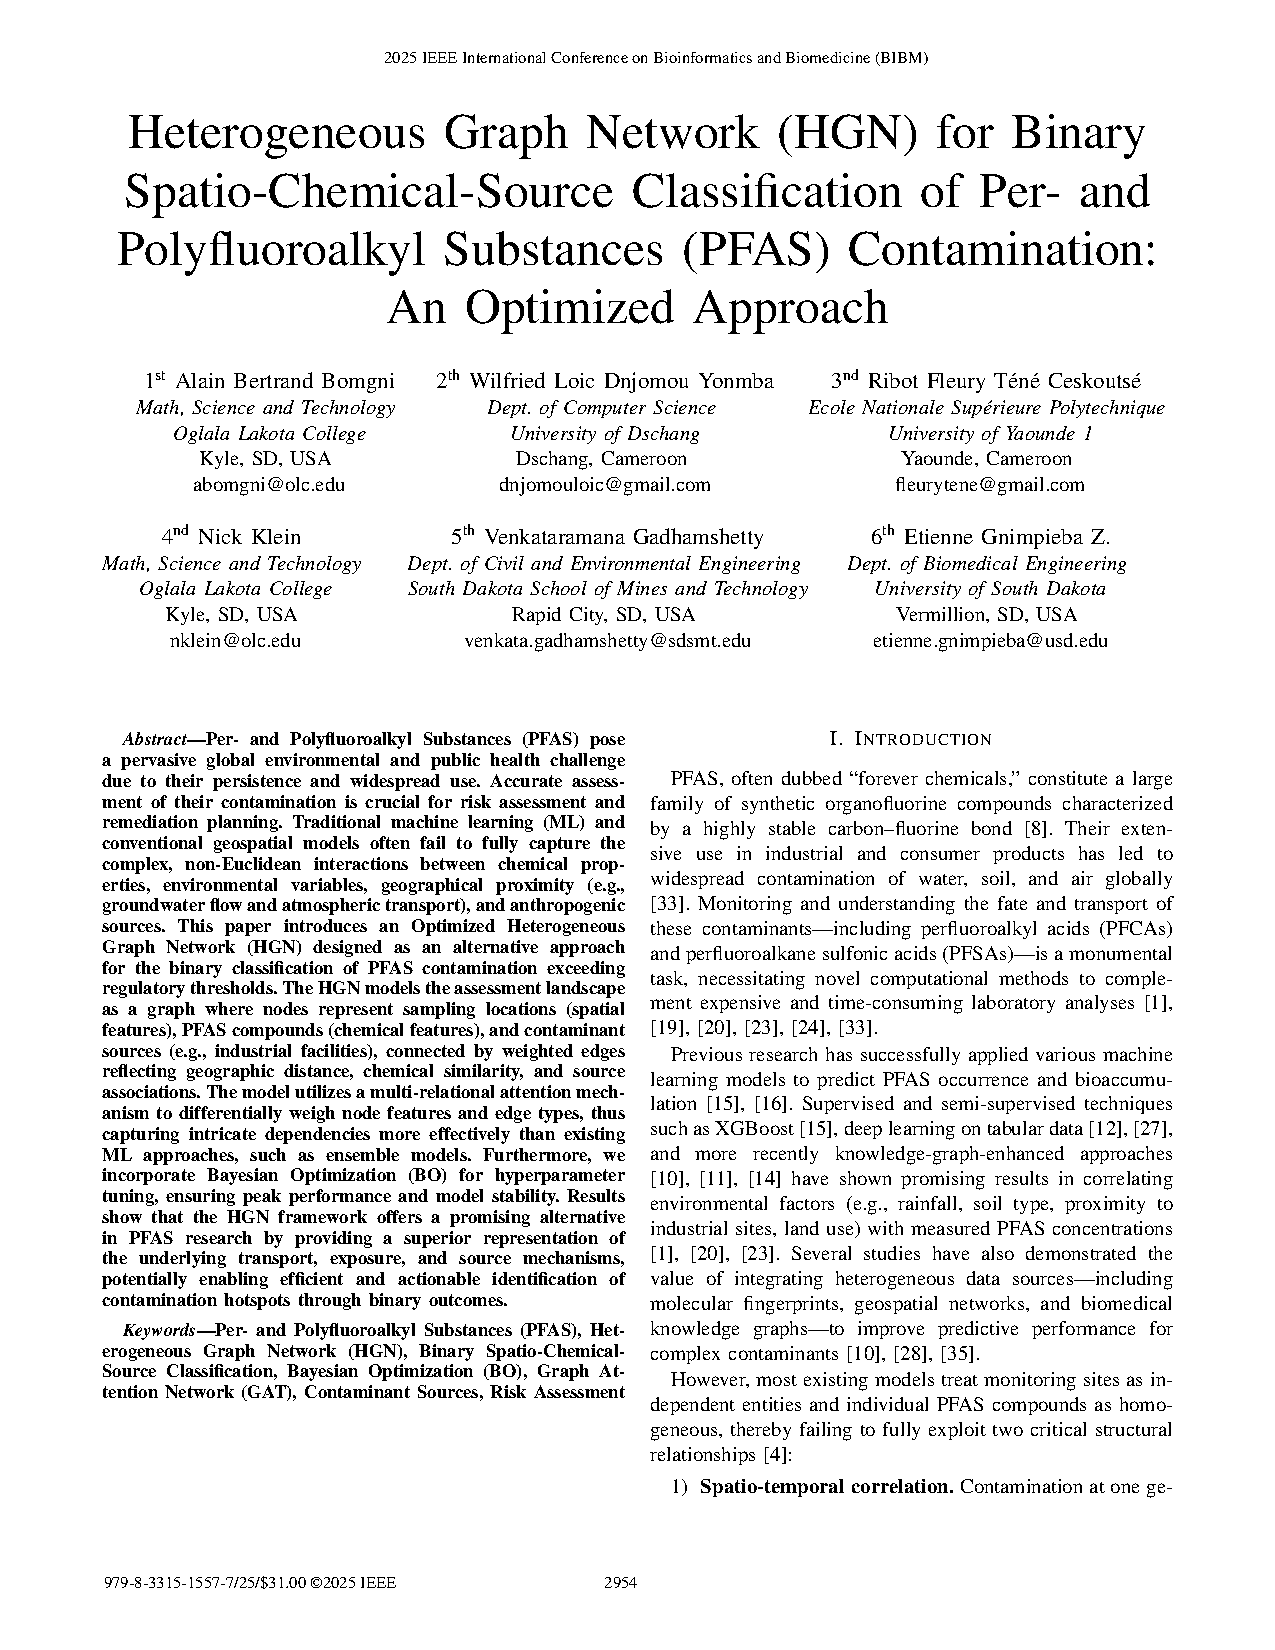
\includegraphics[page=1,width=\textwidth,height=0.95\textheight,keepaspectratio]{Appendices/S42220.pdf}\par}
\clearpage
{\centering\includegraphics[page=2,width=\textwidth,height=0.95\textheight,keepaspectratio]{Appendices/S42220.pdf}\par}
\clearpage
{\centering\includegraphics[page=3,width=\textwidth,height=0.95\textheight,keepaspectratio]{Appendices/S42220.pdf}\par}
\clearpage
{\centering\includegraphics[page=4,width=\textwidth,height=0.95\textheight,keepaspectratio]{Appendices/S42220.pdf}\par}
\clearpage
{\centering\includegraphics[page=5,width=\textwidth,height=0.95\textheight,keepaspectratio]{Appendices/S42220.pdf}\par}

\myRestoreMarks

	%Ainsi de suite
}
\end{document}
